\section{Годограф Найквиста}

В соответствии с вариантом придумаем три объекта пятого порядка с 
тремя вещественными полюсами и двумя комплексно-сопряженными. Все следующие
передаточные функции (ПФ) объектов были подобраны вручную.
 
\subsection{Объект 1}

ПФ с четырьмя неустойчивыми полюсами у разомкнутой системы и один неустойчивый полюс у замкнутой,
разомкнутая система:
\begin{equation*}
    W_1(s)=\frac{100s^4+100s^3+100s^2+100s-100}{(s-1-j)(s-1+j)(s-2)(s-3)(s+1)}
    = \frac{100s^4+100s^3+100s^2+100s-100}{s^5-6s^4+11s^3-4s^2-10s+12}.
\end{equation*}
Полюса разомкнутой и замкнутой систем можно увидеть в таблице \ref{tab:poles},
как и их изображение на комплексной плоскости на рисунке \ref{fig:obj1_pz}
вместе с нулями. Из 4 неустойчивых корней остался только 1, значит по критерию 
Найквиста разность между оборотами АФЧХ вокруг (-1; 0) против часовой стрелки и по часовой стрелке
равняется 3.

\begin{table}[h!]
    \centering
    \caption{Полюса объекта 1}
    \begin{tabular}{|c|c|}
    \hline
    \textbf{Полюса разомкнутой системы}       & \textbf{Полюса замкнутой системы}        \\ \hline
    $3.0000 + 0.0000i$ & $-92.8151 + 0.0000i$ \\ \hline
    $-1.0000 + 0.0000i$ & $-1.3498 + 0.0000i$ \\ \hline
    $2.0000 + 0.0000i$ & $-0.1663 + 1.1765i$  \\ \hline
    $1.0000 + 1.0000i$ & $-0.1663 - 1.1765i$  \\ \hline
    $1.0000 - 1.0000i$ & $0.4975 + 0.0000i$   \\ \hline
    \end{tabular}
    \label{tab:poles}
\end{table}
    

\begin{figure}[H]
    \centering
    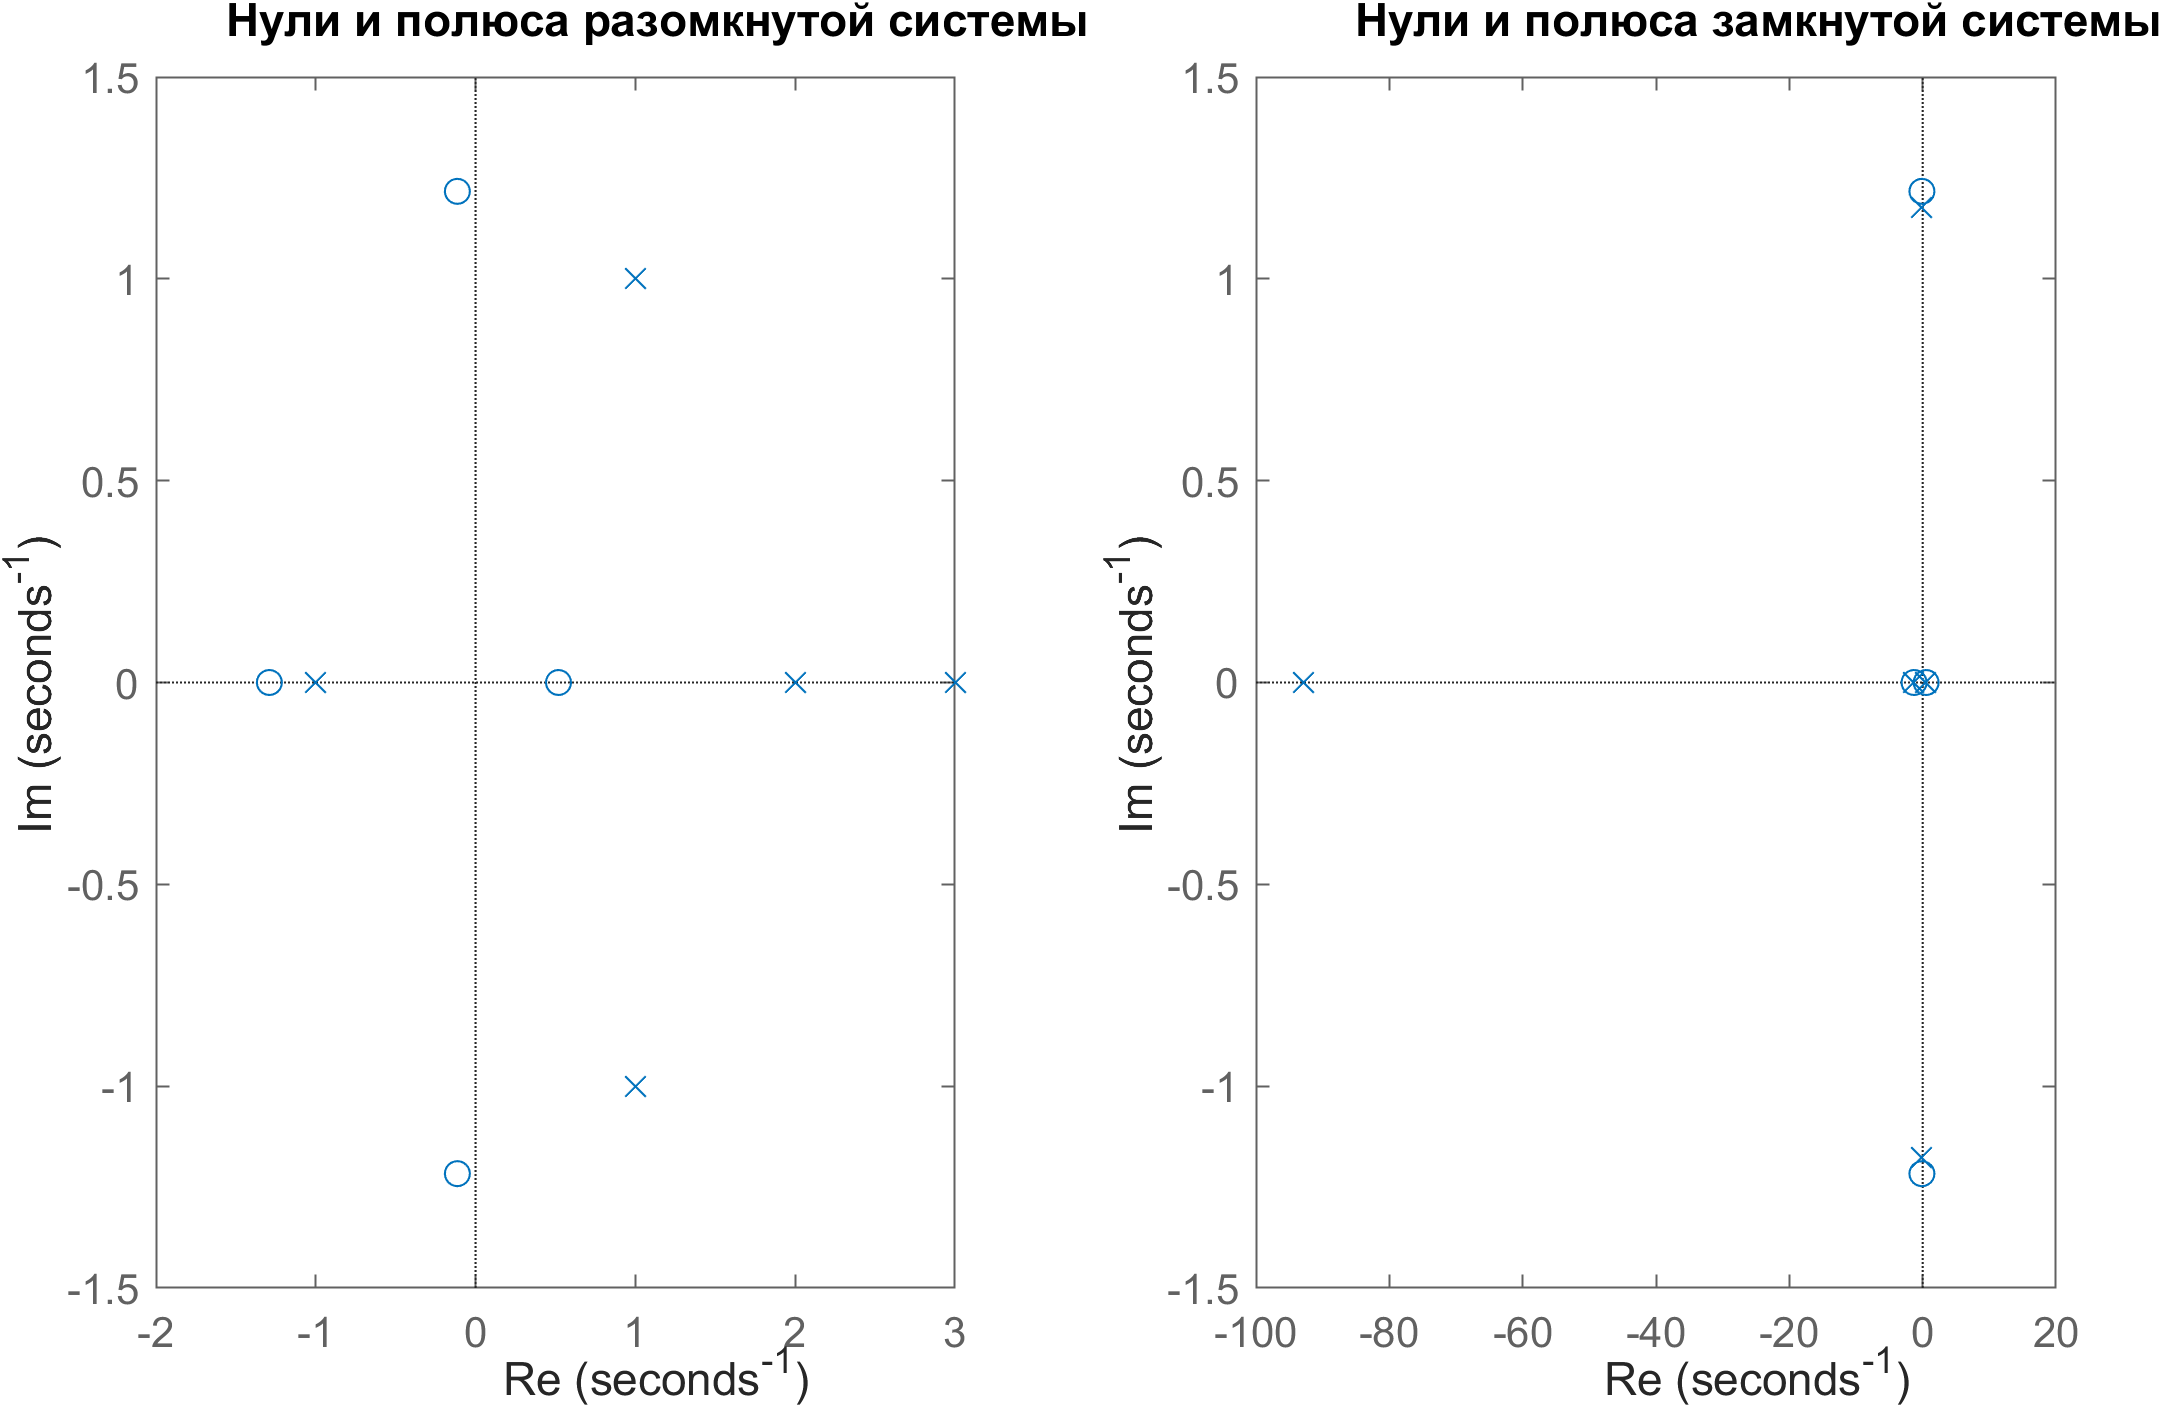
\includegraphics[width=\textwidth]{figs/task_1_obj_1_zeros_poles.png}
    \caption{Нули и полюса объекта 1}
    \label{fig:obj1_pz}
\end{figure}

\begin{figure}[H]
    \centering
    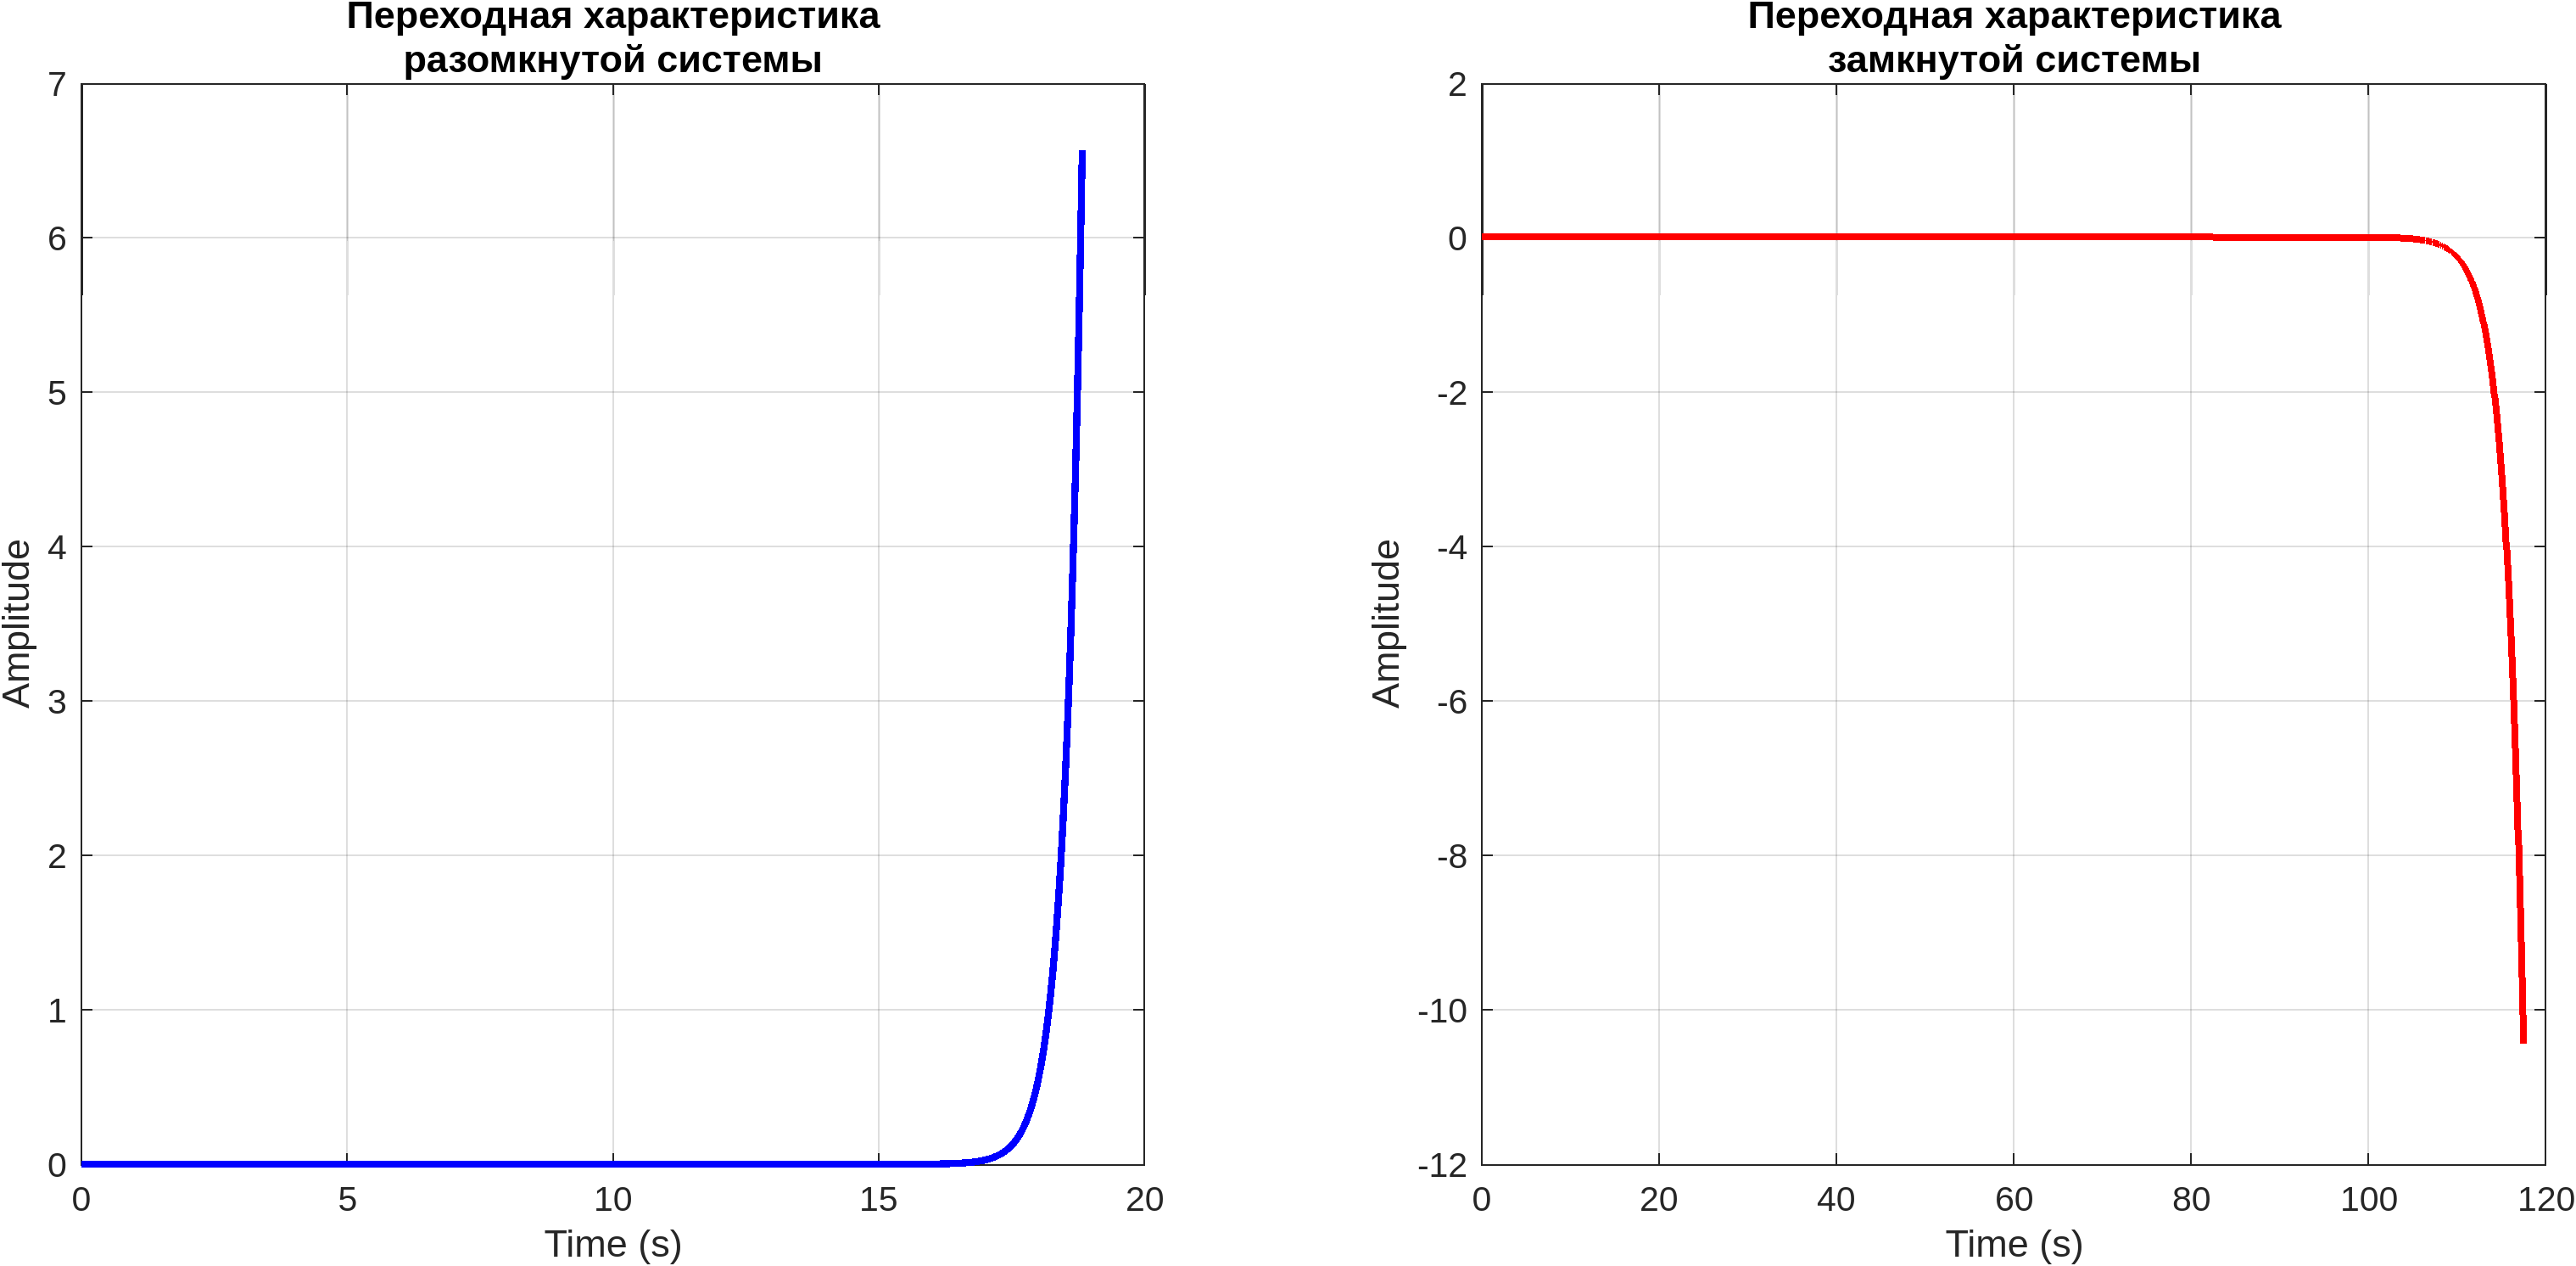
\includegraphics[width=\textwidth]{figs/task_1_obj_1_step.png}
    \caption{Переходные характеристики объекта 1}
    \label{fig:obj1_step}
\end{figure}

\begin{figure}[H]
    \centering
    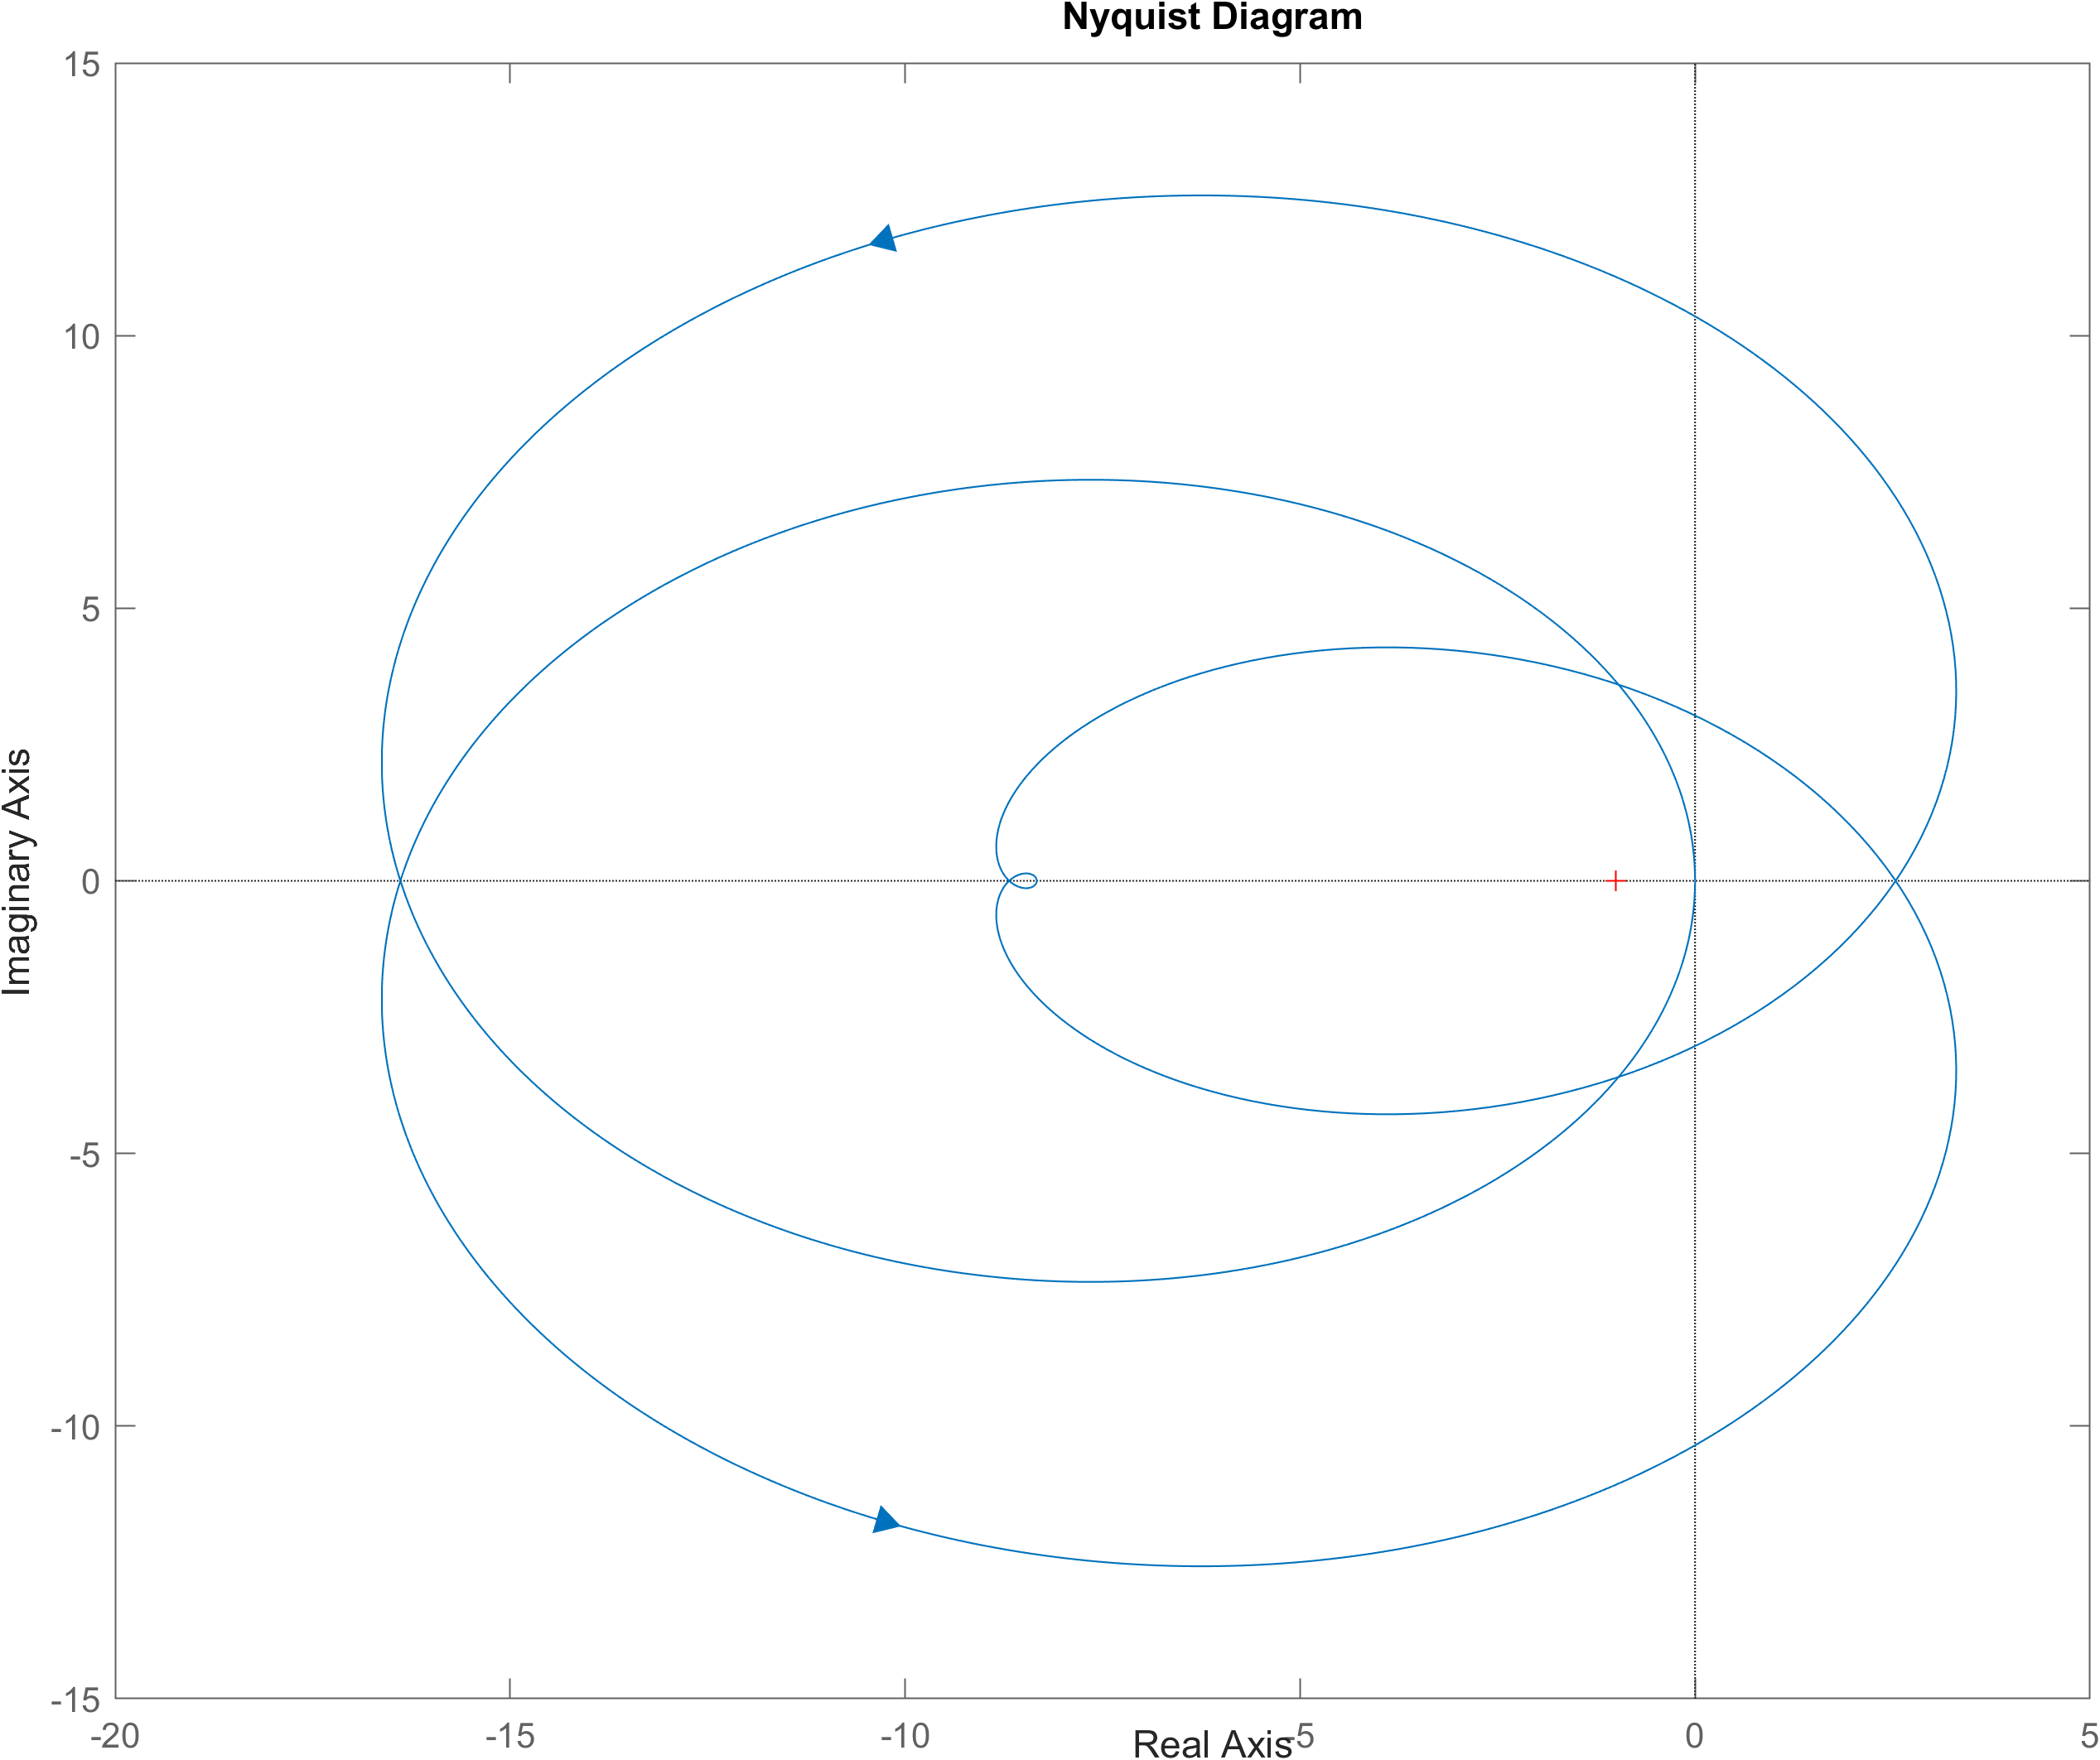
\includegraphics[width=\textwidth]{figs/task_1_obj_1_nyquist.png}
    \caption{Годограф Найквиста объекта 1}
    \label{fig:obj1_nyquist}
\end{figure}

\begin{figure}[H]
    \centering
    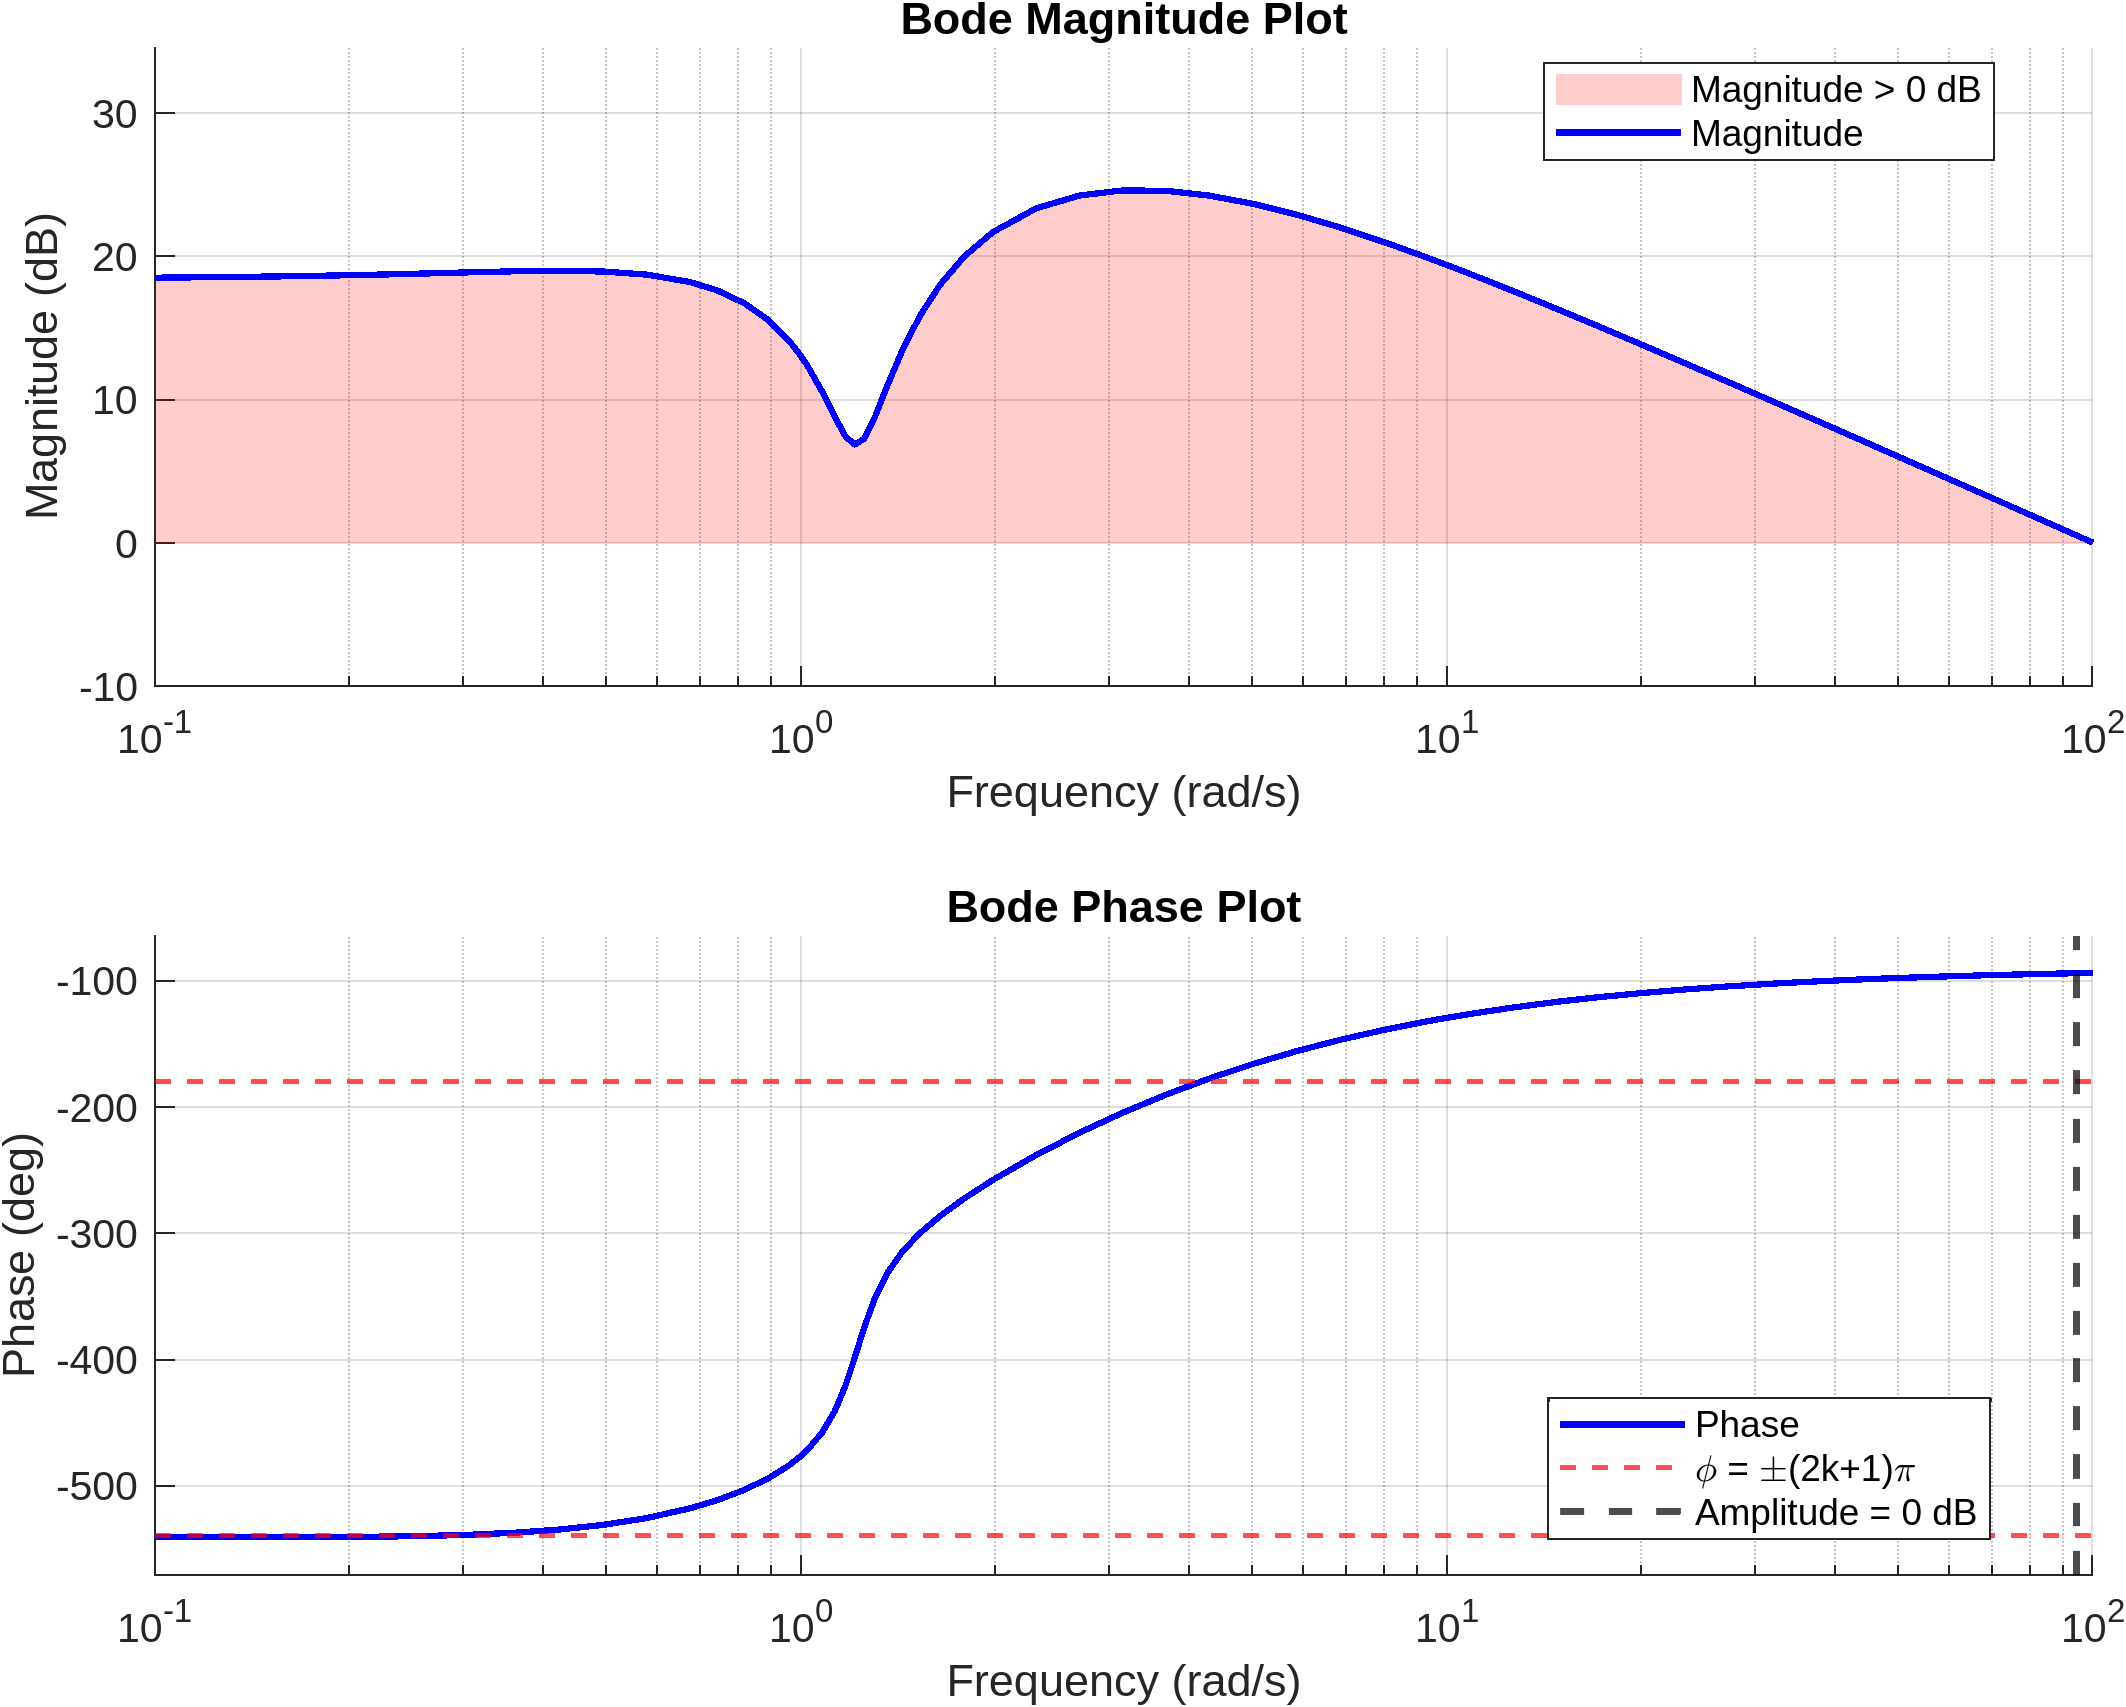
\includegraphics[width=\textwidth]{figs/task_1_obj_1_bode.png}
    \caption{ЛАФЧХ разомкнутой системы объекта 1}
    \label{fig:obj1_bode}
\end{figure}

Переходные характеристики можно увидеть на рисунке \ref{fig:obj1_step},
системы расходятся. Годограф Найквиста можно увидеть на рисунке 
\ref{fig:obj1_nyquist}, как видно, число оборотов против часовой стрелки
вокруг (-1; 0) равняется 3, что соответствует выводам по критерию Найквиста
выше. ЛАФЧХ разомкнутой системы можно увидеть на рисунке \ref{fig:obj1_bode},
воспользовавшись логарифмическим критерием Найквиста, убеждаемся, что 
закнутая система не будет устойчива, так как переходов $\frac{3}{2}$, а нужно $2$.


\newpage
\subsection{Объект 2}

ПФ без неустойчивых полюсов у разомкнутой системы и с одним неустойчивым полюсом у замкнутой,
разомкнутая система:
\begin{equation*}
    W_2(s)=\frac{-100}{(s+1+j)(s+1-j)(s+2)(s+3)(s+4)}=
    \frac{-100}{s^5+11s^4+46s^3+194s^2+100s+48}.
\end{equation*}

Полюса разомкнутой и замкнутой систем можно увидеть в таблице \ref{tab:poles2},
как и их изображение на комплексной плоскости на рисунке \ref{fig:obj2_pz}
вместе с нулями. Неустойчивых корней не было, появился 1, значит по критерию 
Найквиста разность между оборотами АФЧХ вокруг (-1; 0) против часовой стрелки и по часовой стрелке
равняется -1.

\begin{table}[H]
    \centering
    \caption{Полюса объекта 2}
    \begin{tabular}{|c|c|}
    \hline
    \textbf{Полюса разомкнутой системы}       & \textbf{Полюса замкнутой системы}        \\ \hline
    $-8.1009 + 0.0000i$      & $-8.0765 + 0.0000i$        \\ \hline
    $-1.1890 + 4.4248i$      & $-1.1348 + 4.4632i$        \\ \hline
    $-1.1890 - 4.4248i$      & $-1.1348 - 4.4632i$        \\ \hline
    $-0.2606 + 0.4630i$      & $-0.9676 + 0.0000i$        \\ \hline
    $-0.2606 - 0.4630i$      & $0.3137 + 0.0000i$         \\ \hline
    \end{tabular}
    \label{tab:poles2}
\end{table}
    

\begin{figure}[H]
    \centering
    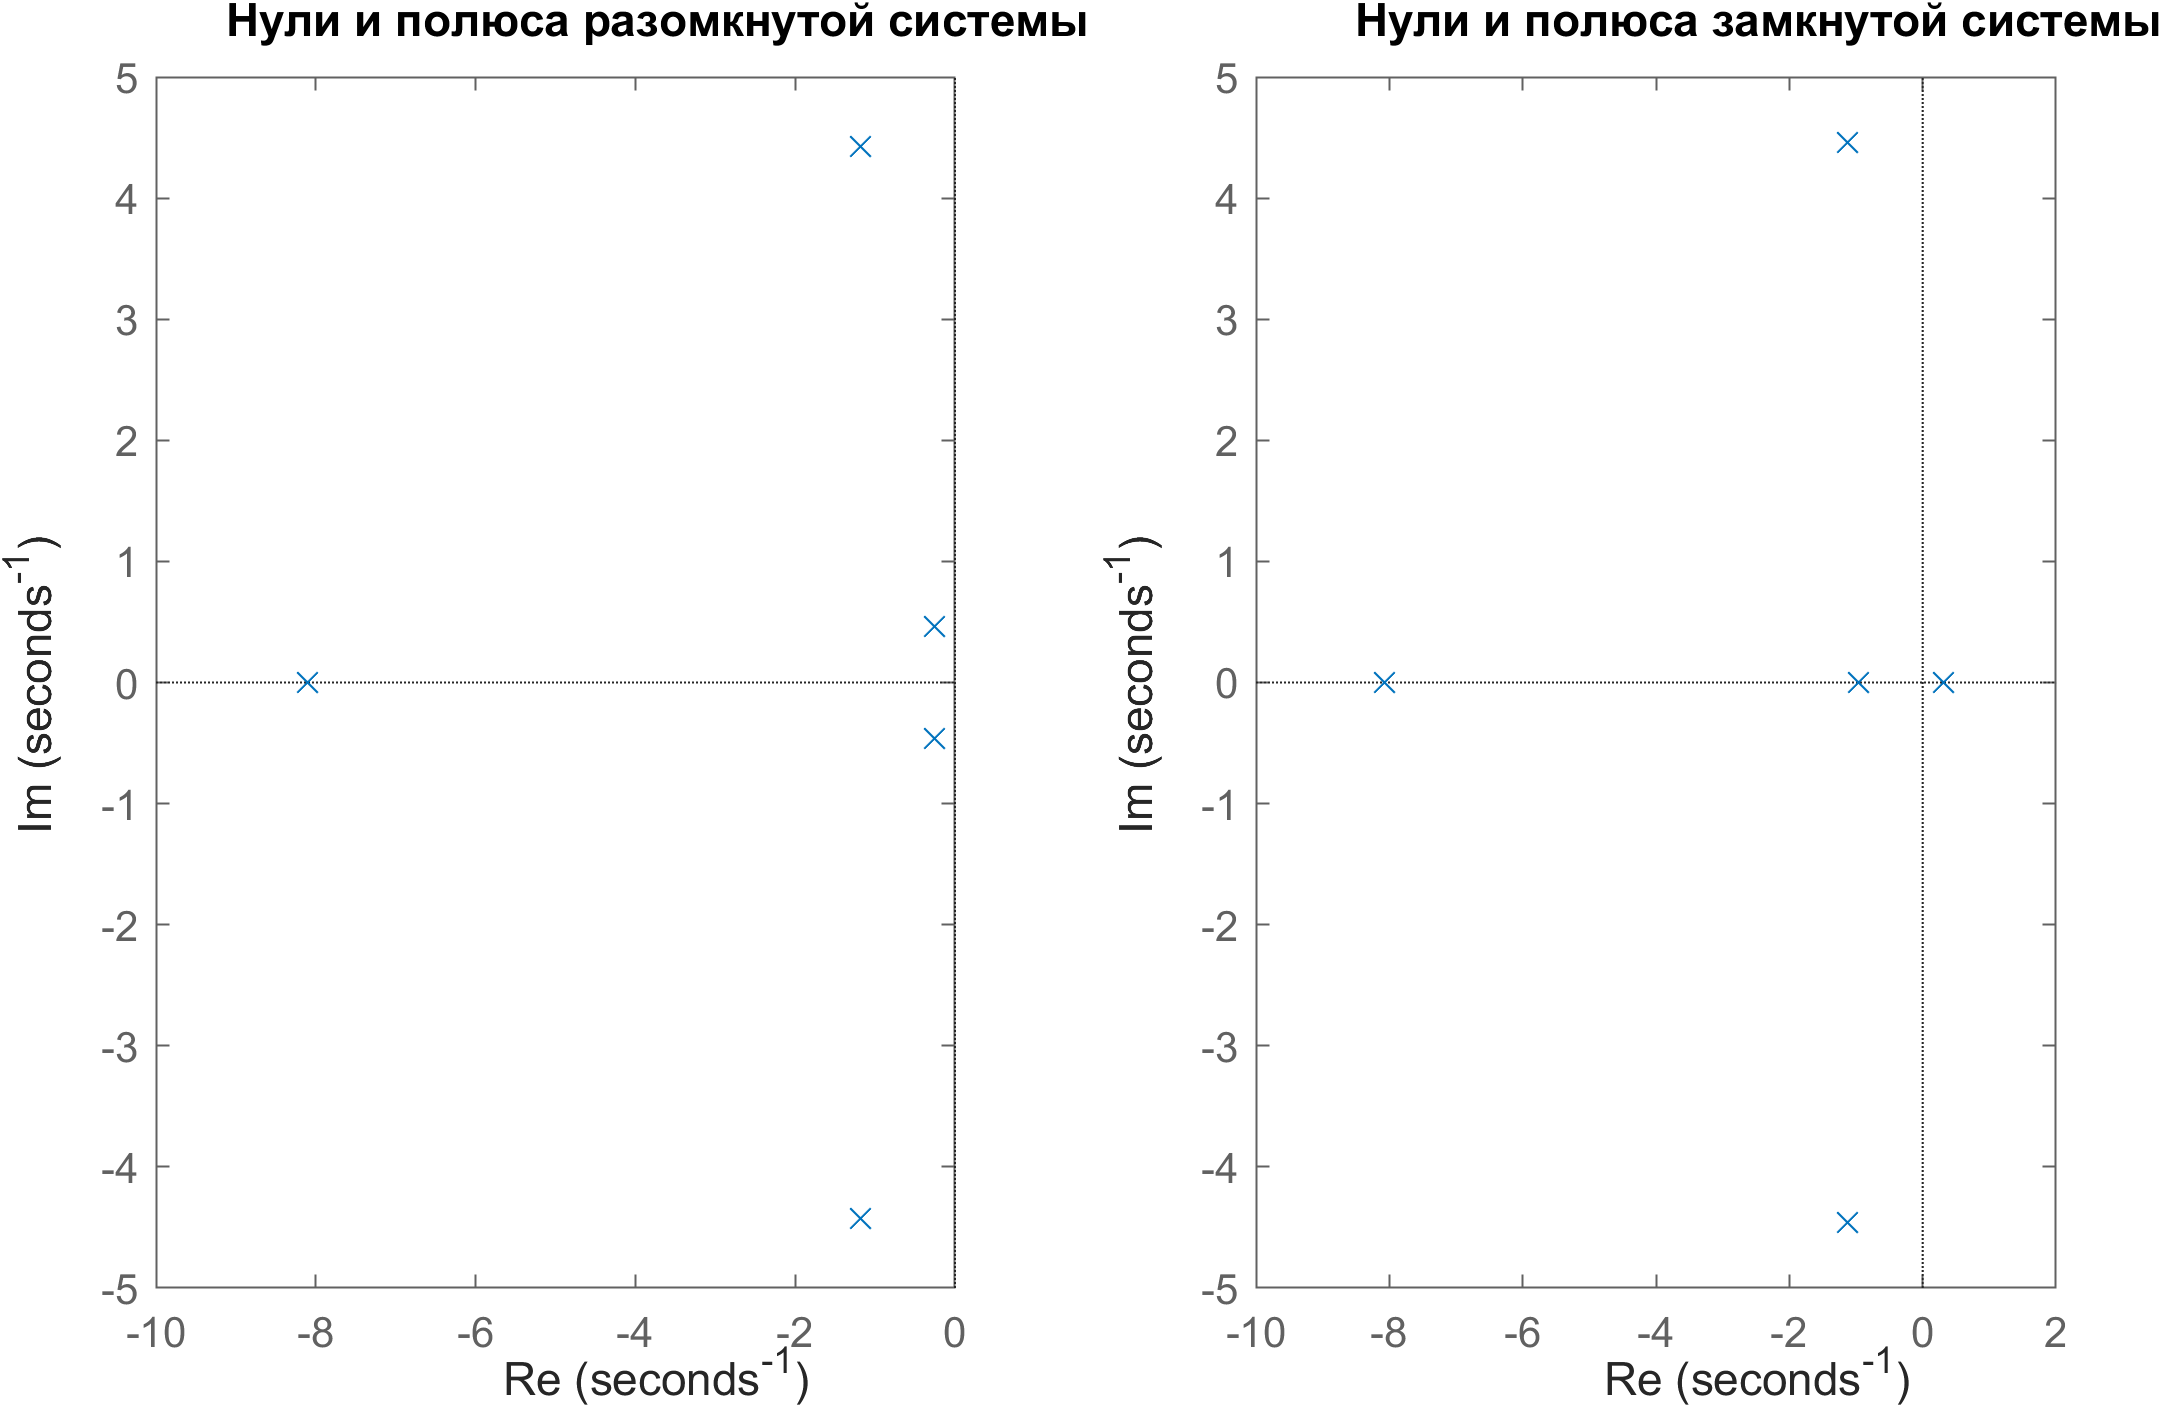
\includegraphics[width=\textwidth]{figs/task_1_obj_2_zeros_poles.png}
    \caption{Нули и полюса объекта 2}
    \label{fig:obj2_pz}
\end{figure}

\begin{figure}[H]
    \centering
    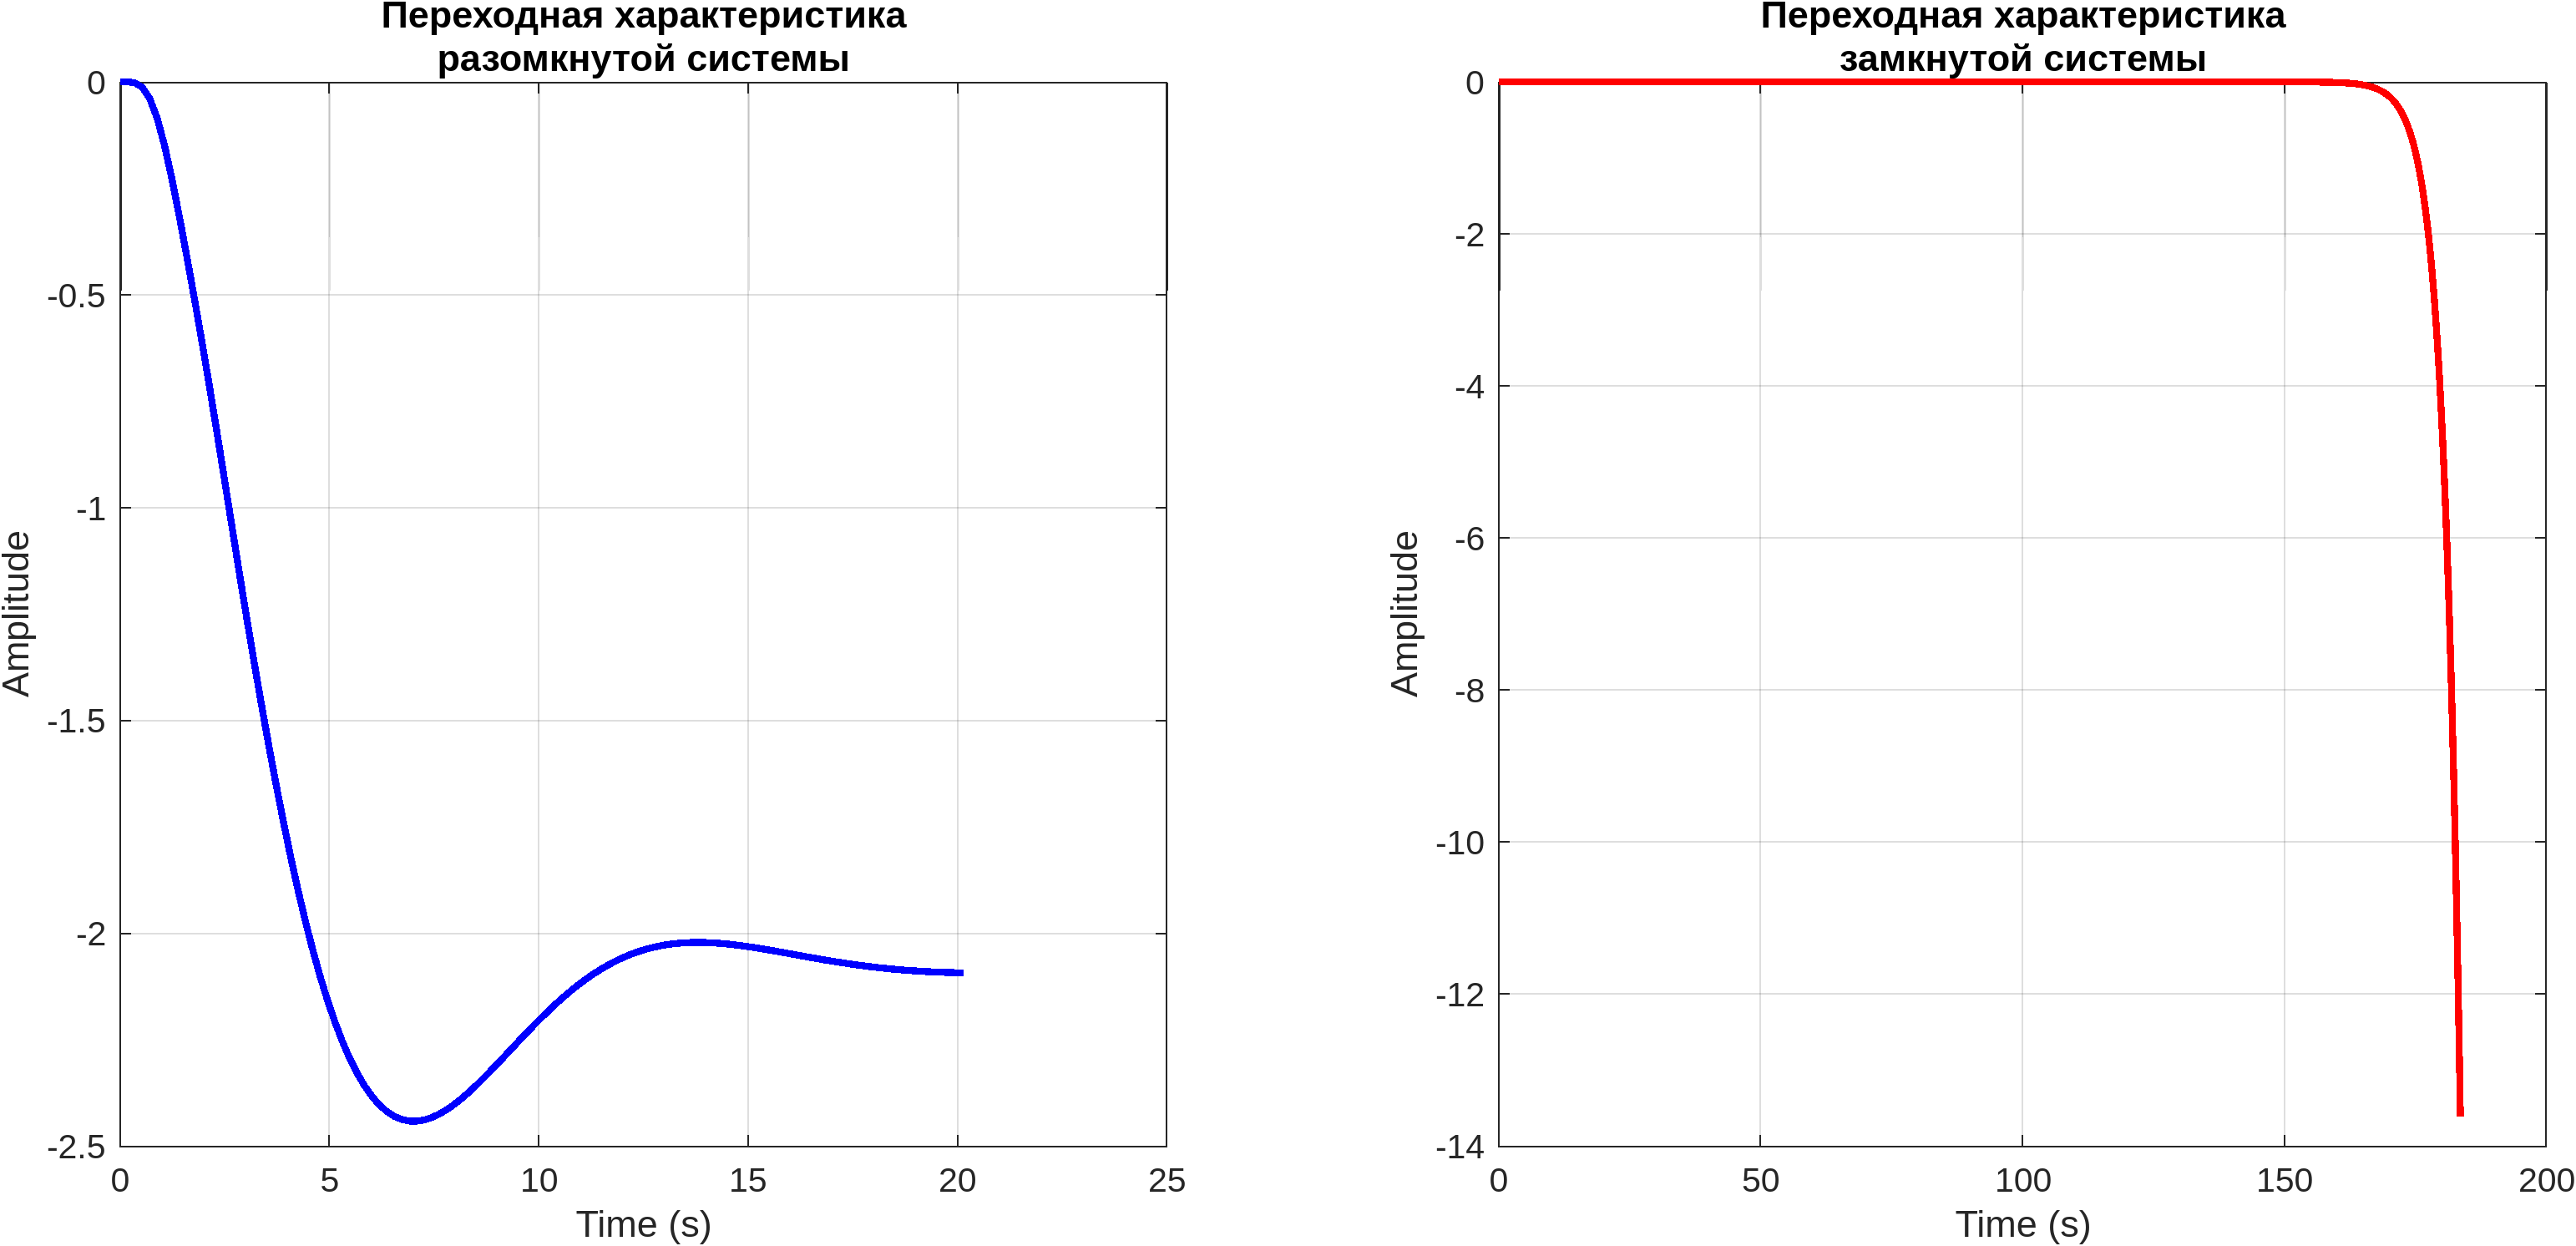
\includegraphics[width=\textwidth]{figs/task_1_obj_2_step.png}
    \caption{Переходные характеристики объекта 2}
    \label{fig:obj2_step}
\end{figure}

\begin{figure}[H]
    \centering
    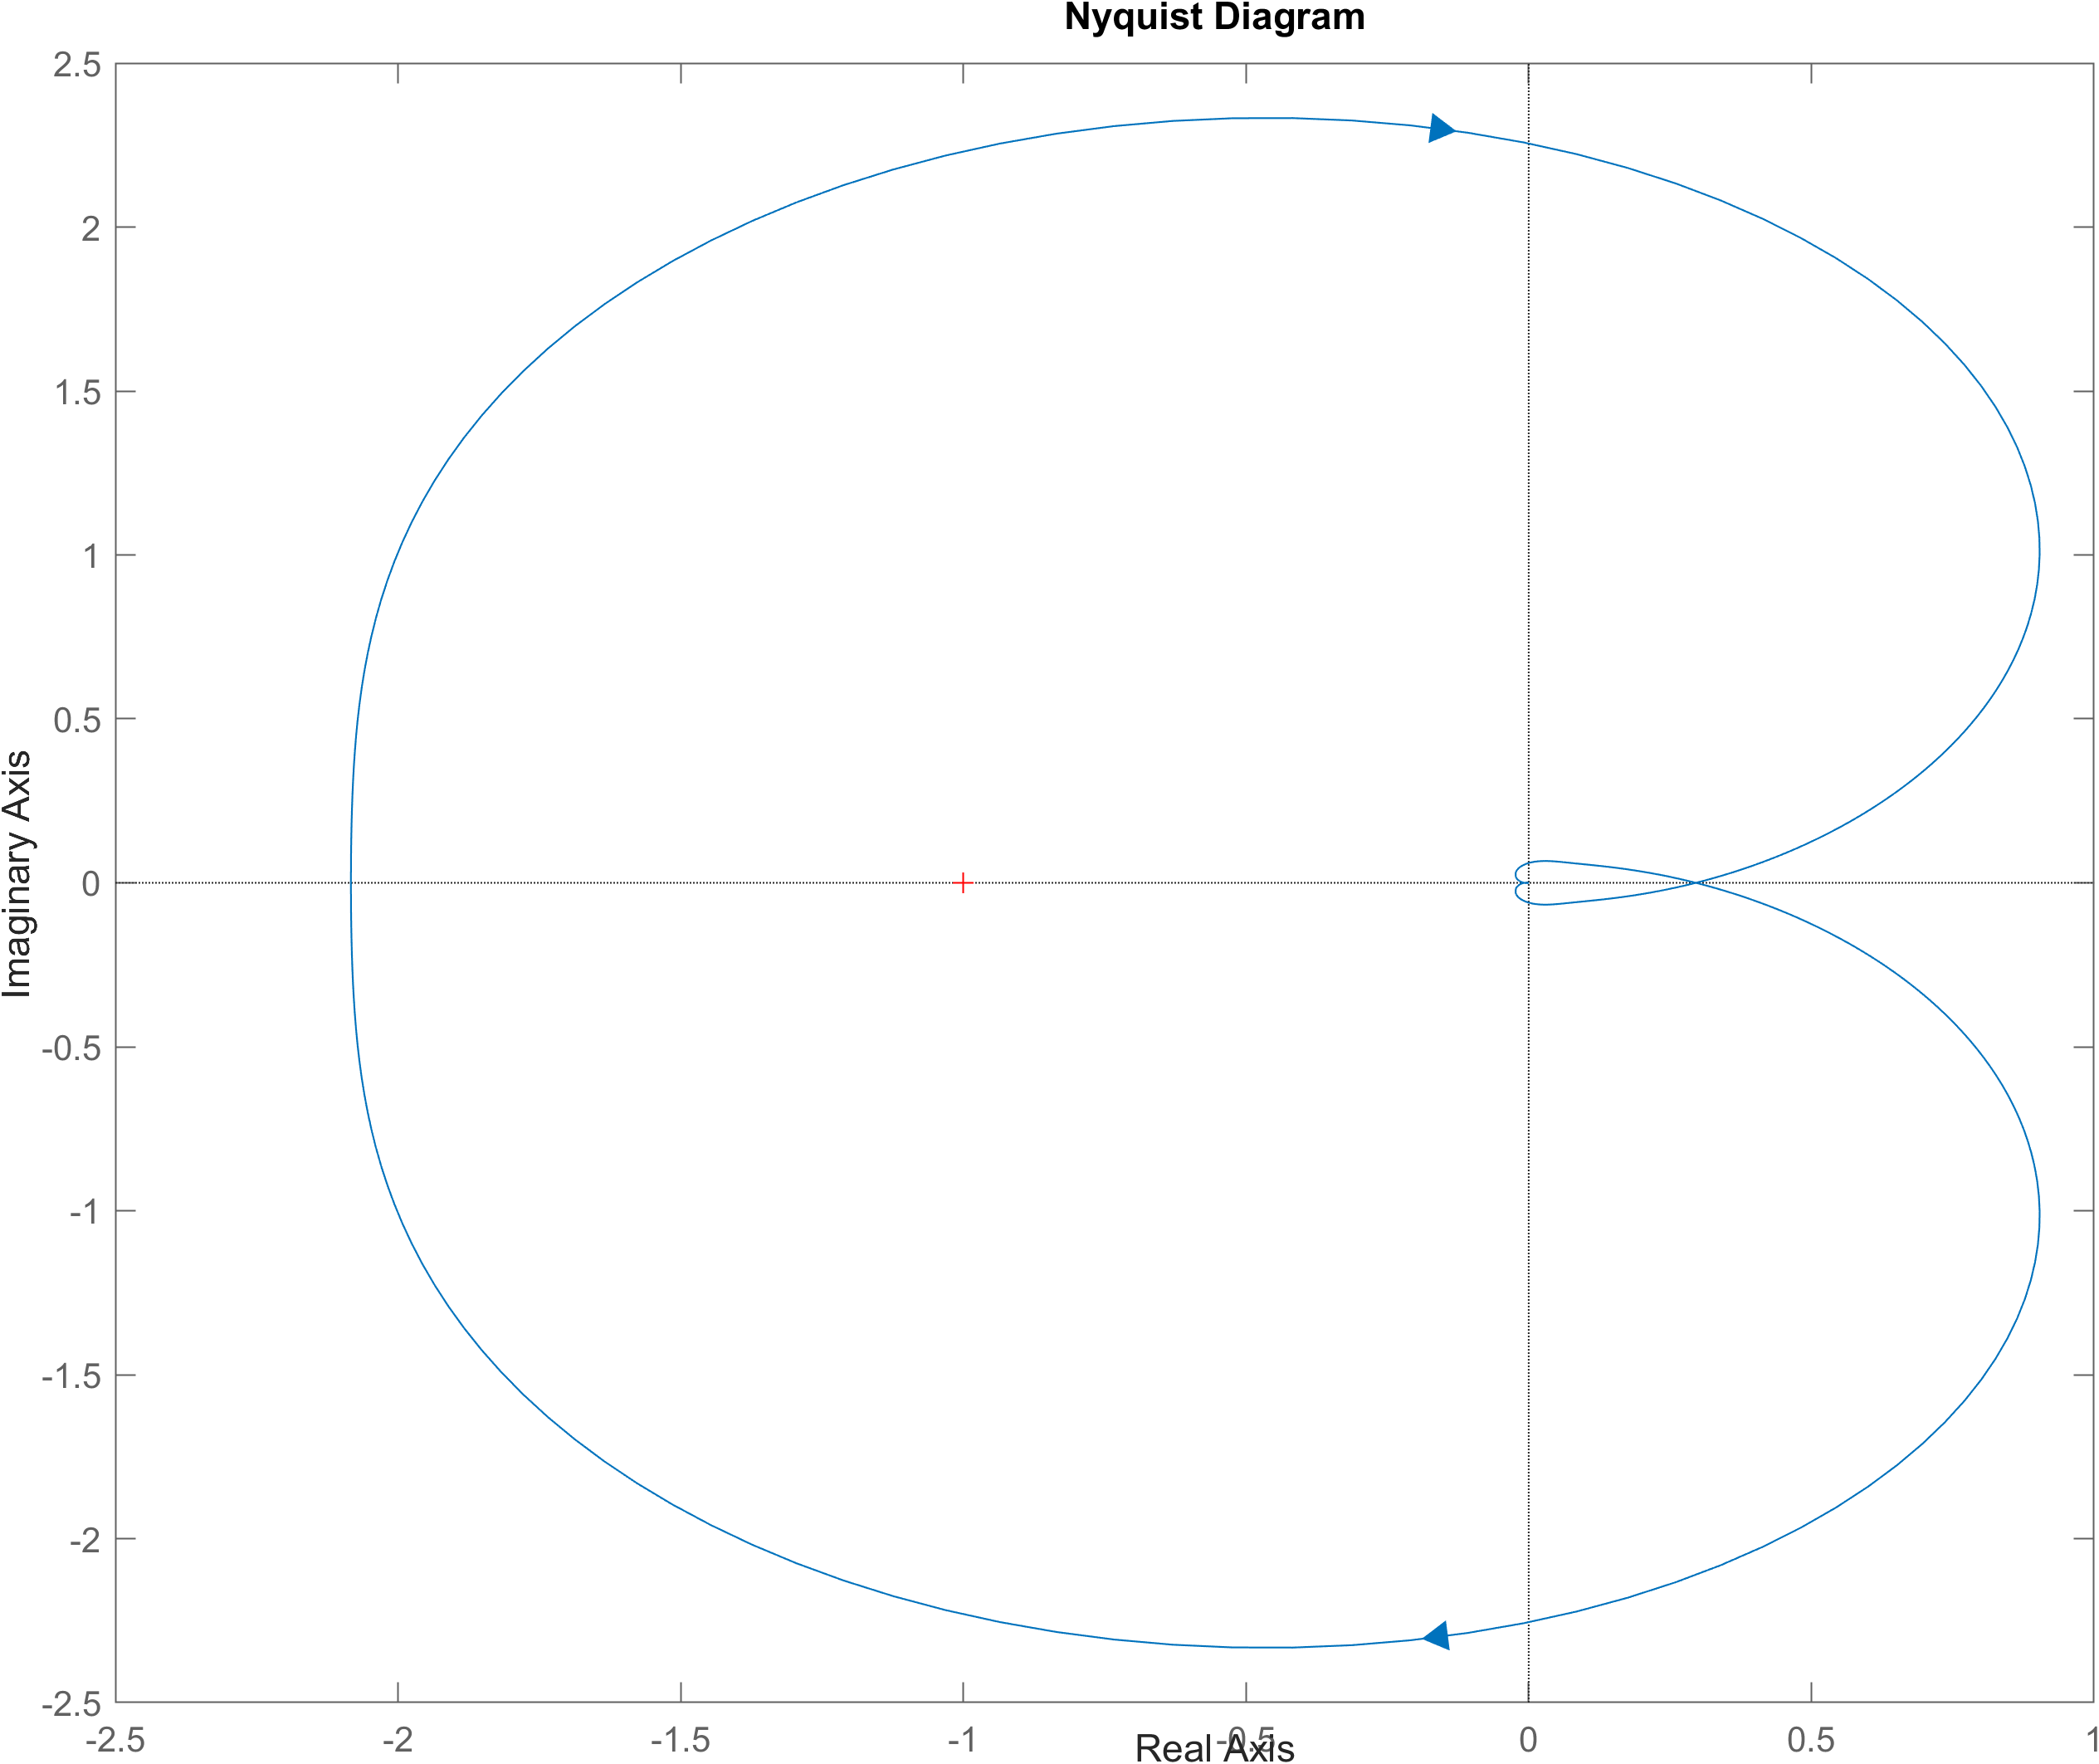
\includegraphics[width=\textwidth]{figs/task_1_obj_2_nyquist.png}
    \caption{Годограф Найквиста объекта 2}
    \label{fig:obj2_nyquist}
\end{figure}

\begin{figure}[H]
    \centering
    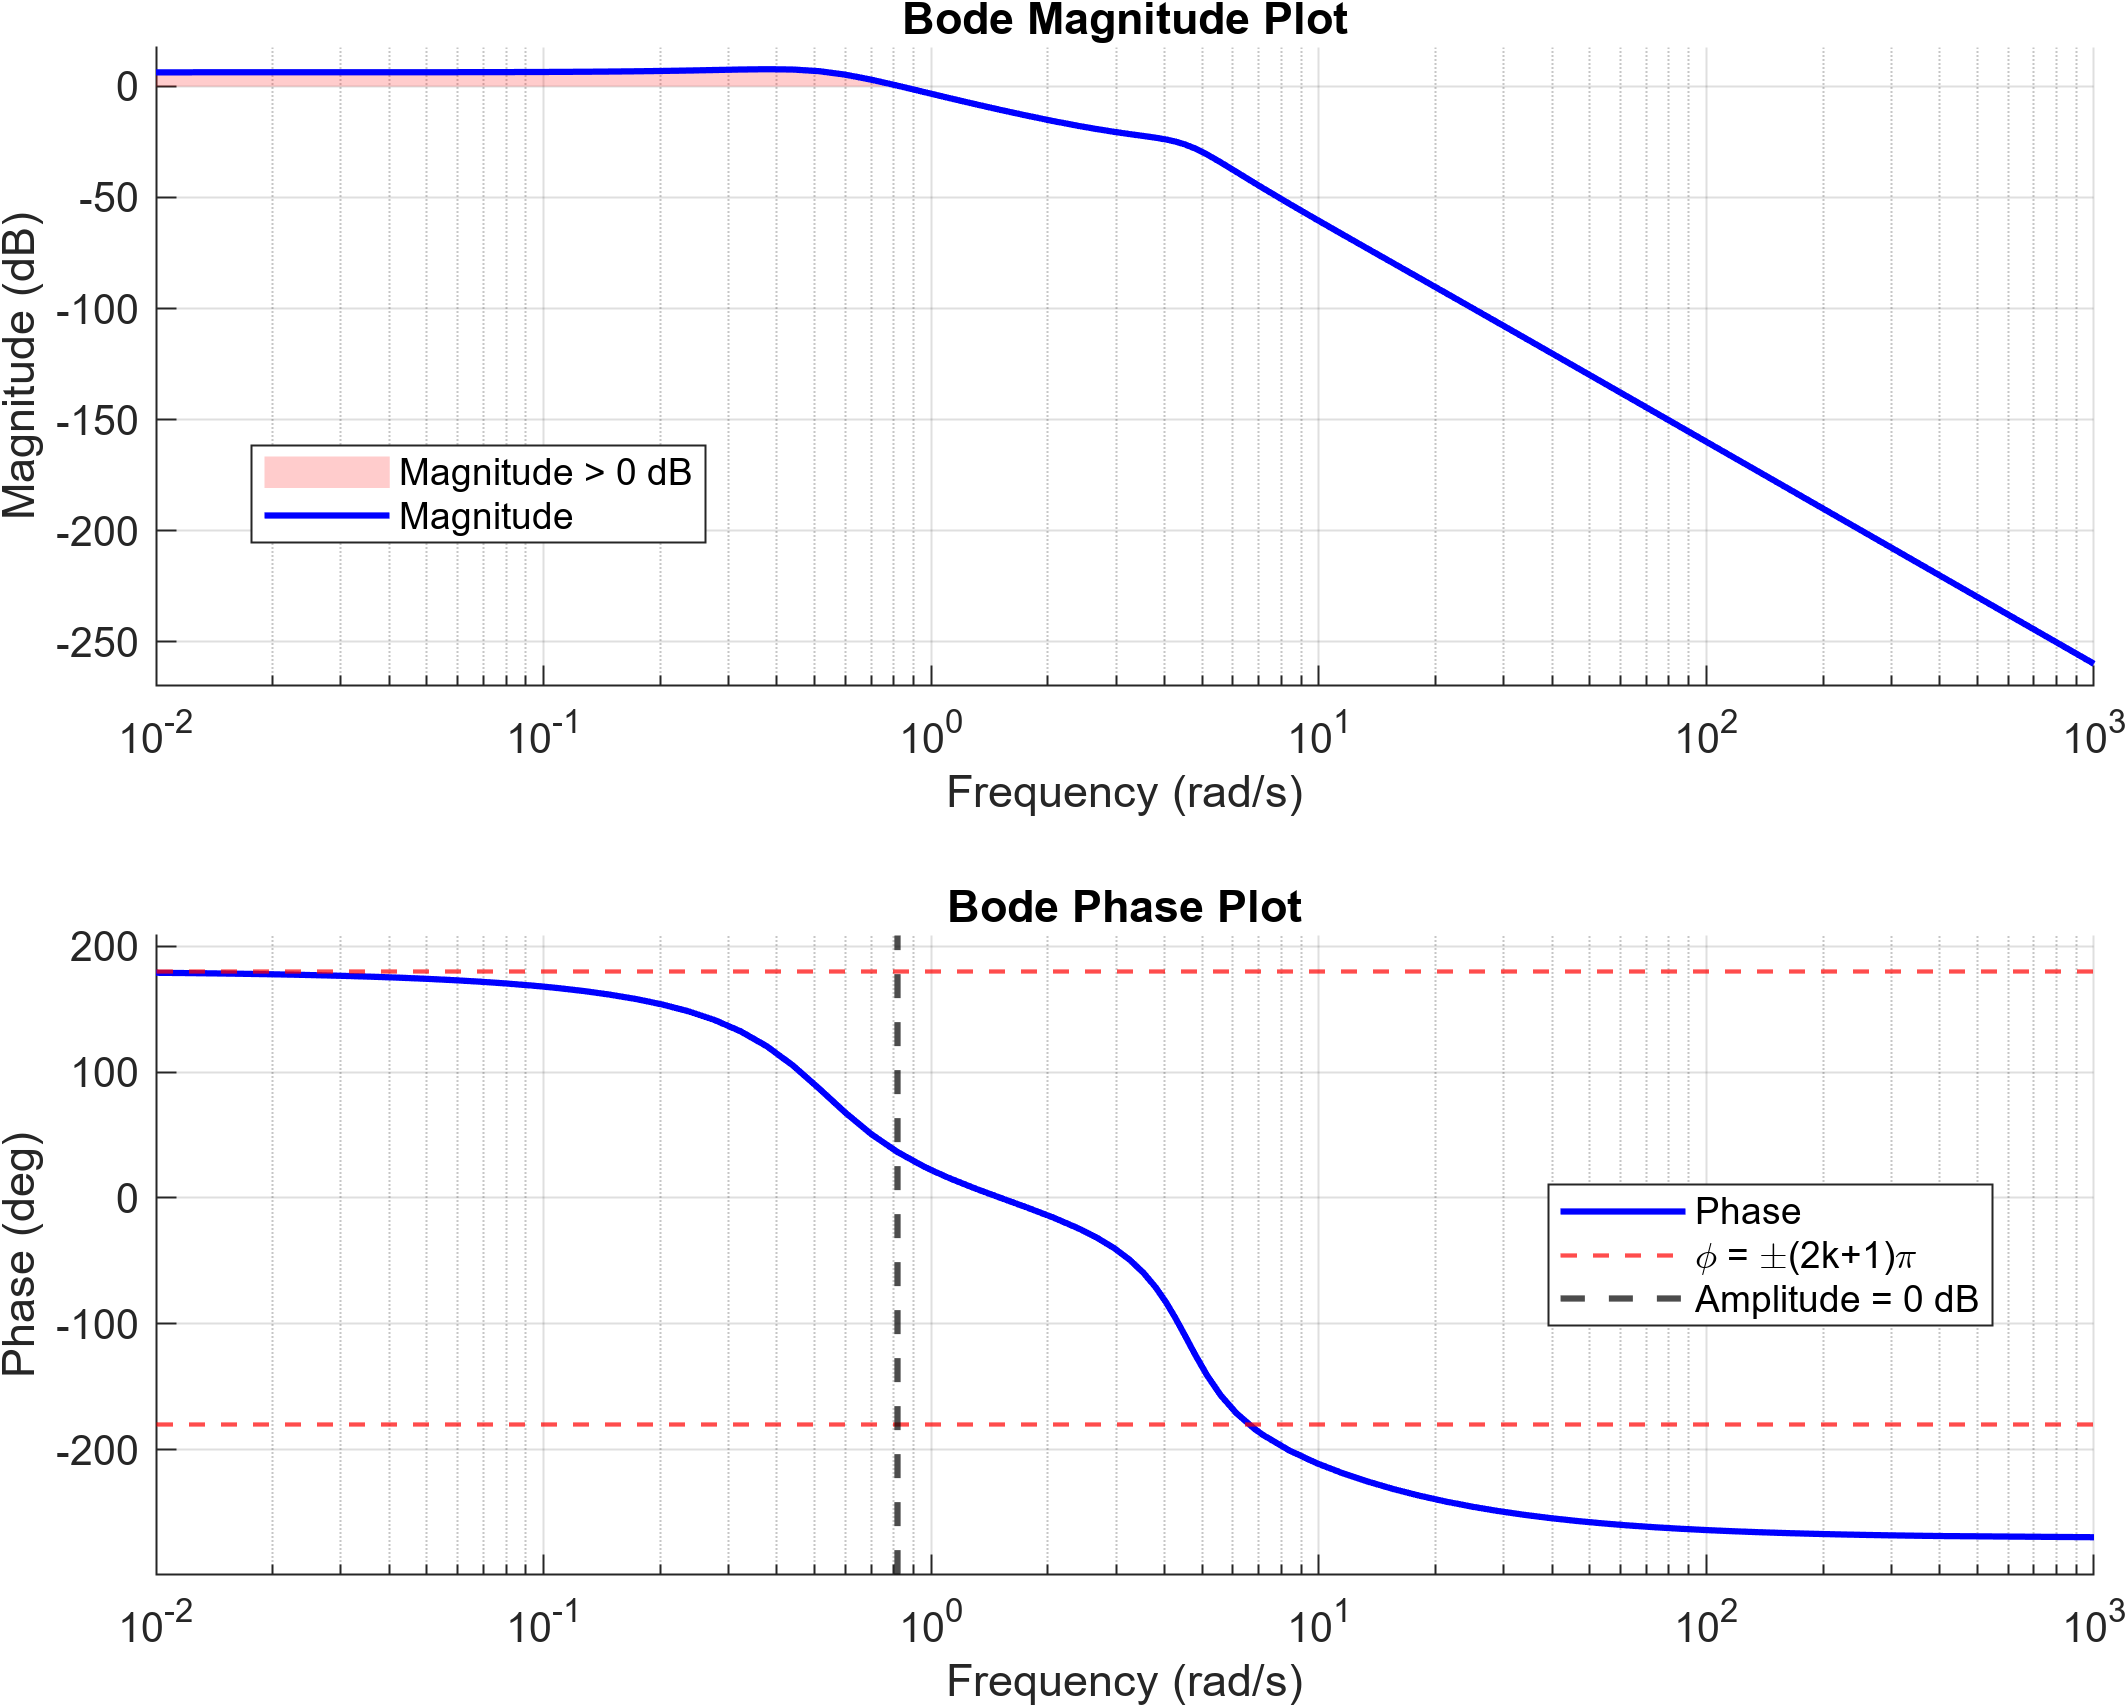
\includegraphics[width=\textwidth]{figs/task_1_obj_2_bode.png}
    \caption{ЛАФЧХ разомкнутой системы объекта 2}
    \label{fig:obj2_bode}
\end{figure}

Переходные характеристики можно увидеть на рисунке \ref{fig:obj2_step},
разомкнутая сходится где-то около -2, а замкнутая расходятся. 
Годограф Найквиста можно увидеть на рисунке 
\ref{fig:obj2_nyquist}, как видно, число оборотов по часовой стрелки
вокруг (-1; 0) равняется 1, что соответствует выводам по критерию Найквиста
выше. ЛАФЧХ разомкнутой системы можно увидеть на рисунке \ref{fig:obj2_bode},
воспользовавшись логарифмическим критерием Найквиста, убеждаемся, что 
замкнутая система не будет устойчива, так как переходов $-\frac{1}{2}$, а нужно $0$.


\newpage
\subsection{Объект 3}

ПФ с четырьмя неустойчивыми полюсами у разомкнутой системы и без таковых у замкнутой,
разомкнутая система:
\begin{equation*}
    W_3(s)=\frac{s^5+31s^4+330s^3+1300s^2+1000s}{(s-1-j)(s-1+j)(s-2)(s-3)(s+1)}
    = \frac{s^5+31s^4+330s^3+1300s^2+1000s}{s^5-6s^4+11s^3-4s^2-10s+12}.
\end{equation*}

Полюса разомкнутой и замкнутой систем можно увидеть в таблице \ref{tab:poles3},
как и их изображение на комплексной плоскости на рисунке \ref{fig:obj3_pz}
вместе с нулями. Было три неустойчивых корня, стало 0, значит по критерию 
Найквиста разность между оборотами АФЧХ вокруг (-1; 0) по часовой стрелки и против часовой стрелке
равняется 4.

\begin{table}[H]
    \centering
    \caption{Полюса объекта 3}
    \begin{tabular}{|c|c|}
    \hline
    \textbf{Полюса разомкнутой системы}       & \textbf{Полюса замкнутой системы}        \\ \hline
        $3.0000 + 0.0000i$ & $-3.8683 + 10.7179i$ \\ \hline
        $-1.0000 + 0.0000i$ & $-3.8683 - 10.7179i$ \\ \hline
        $2.0000 + 0.0000i$ & $-3.7512 + 0.0000i$ \\ \hline
        $1.0000 + 1.0000i$ & $-1.0000 + 0.0000i$ \\ \hline
        $1.0000 - 1.0000i$ & $-0.0123 + 0.0000i$ \\ \hline
    \end{tabular}
    \label{tab:poles3}
\end{table}

\begin{figure}[H]
    \centering
    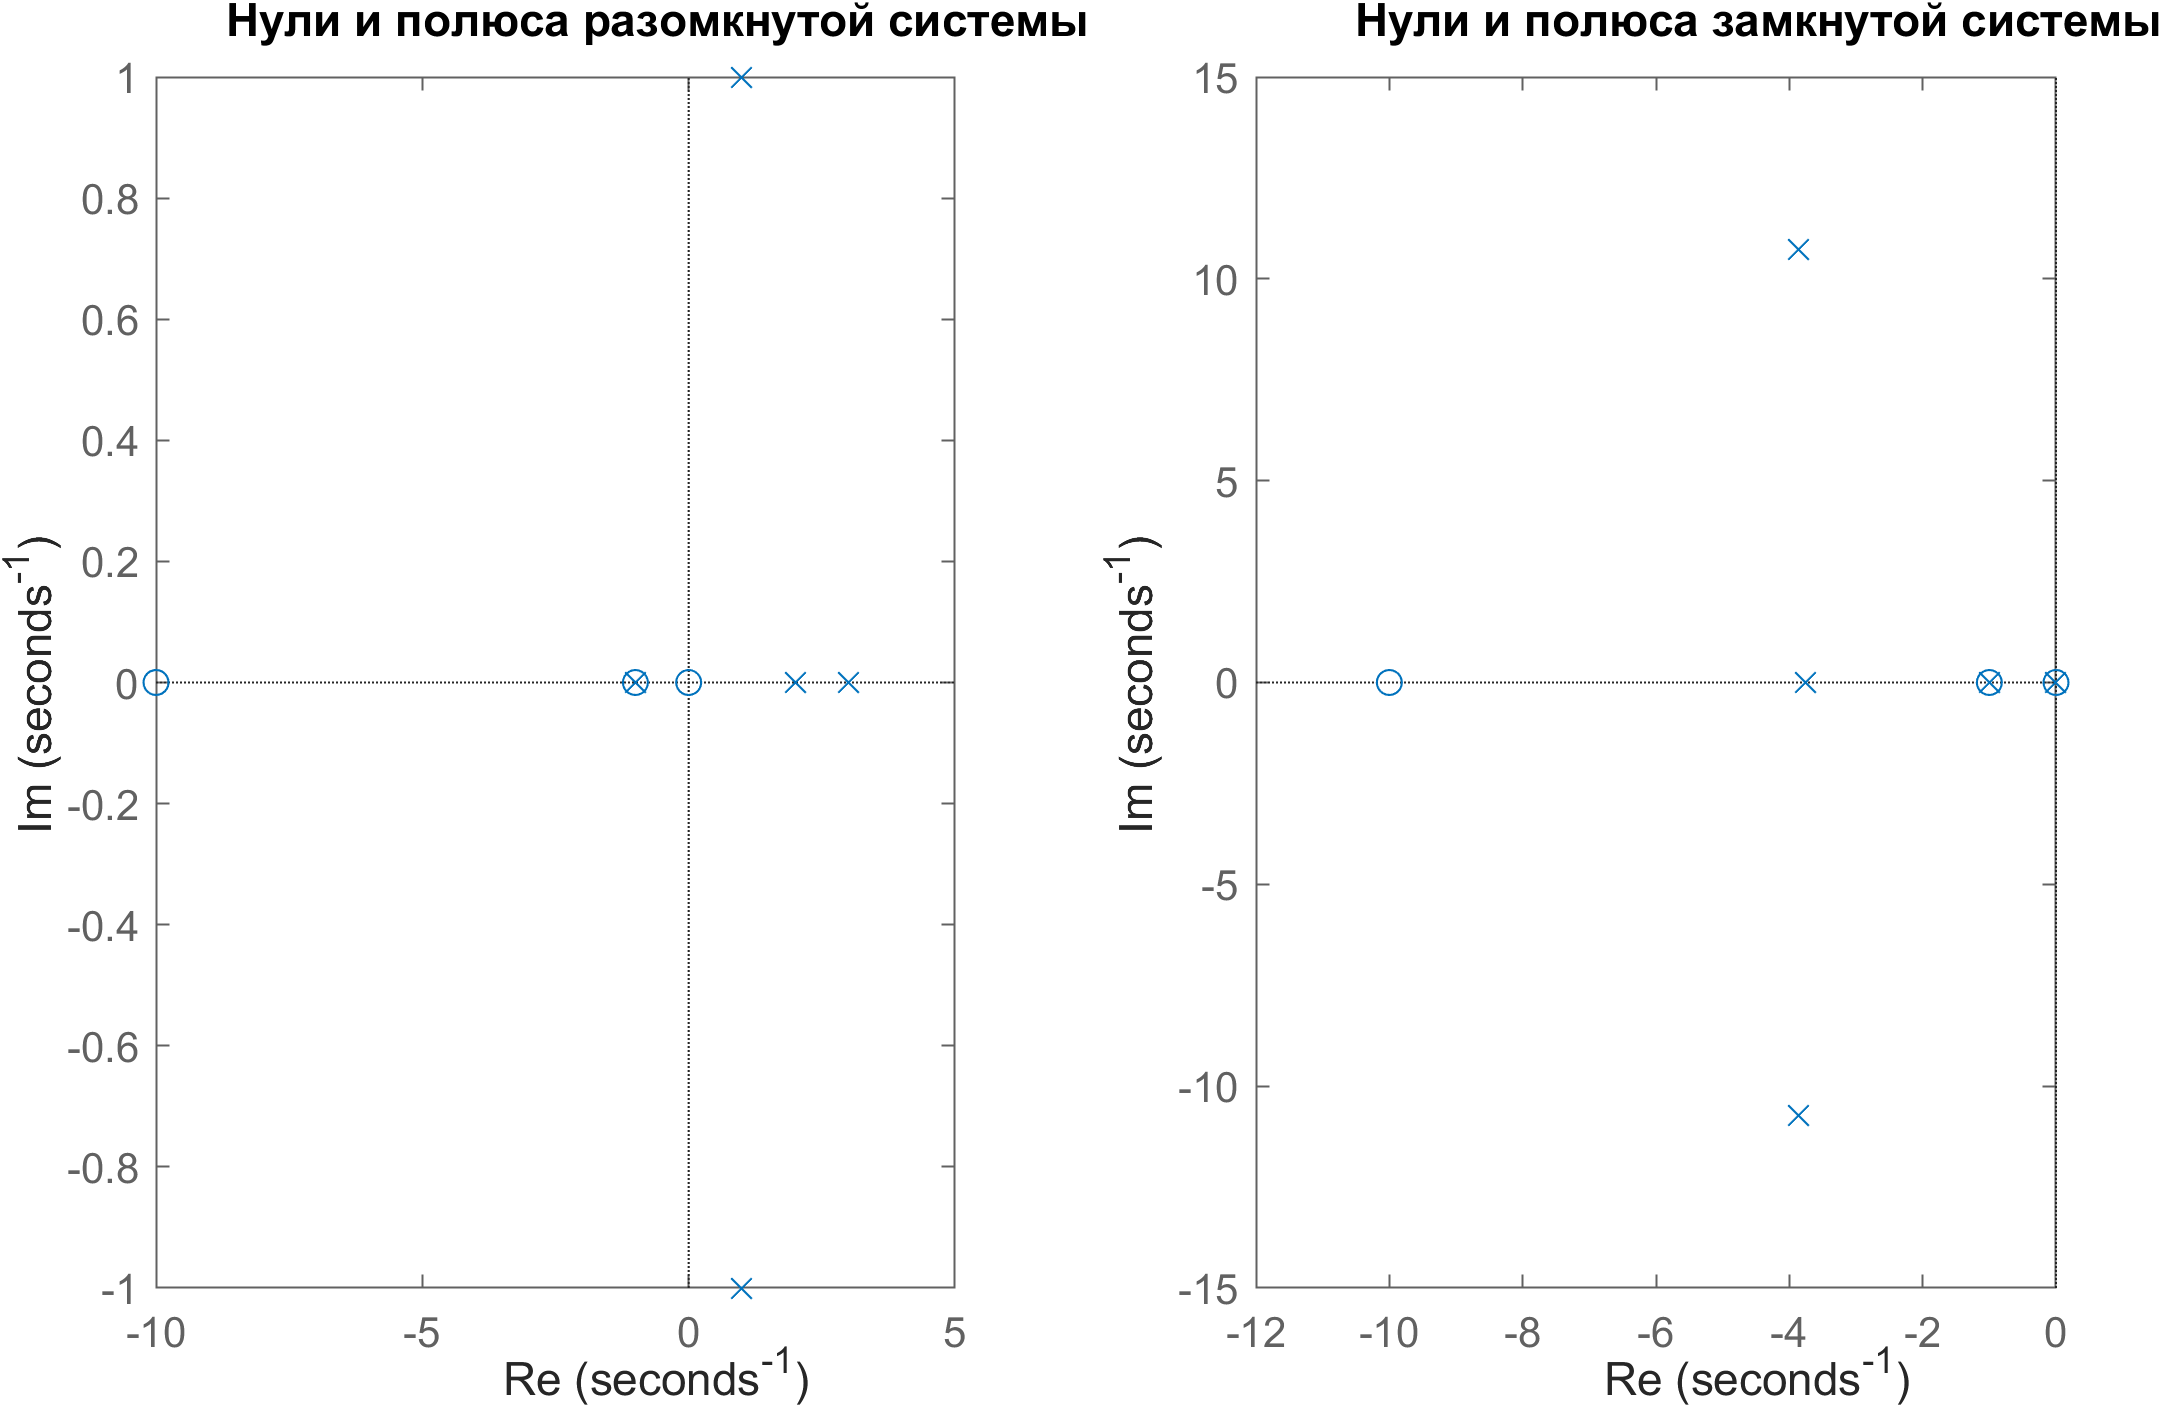
\includegraphics[width=\textwidth]{figs/task_1_obj_3_zeros_poles.png}
    \caption{Нули и полюса объекта 3}
    \label{fig:obj3_pz}
\end{figure}

\begin{figure}[H]
    \centering
    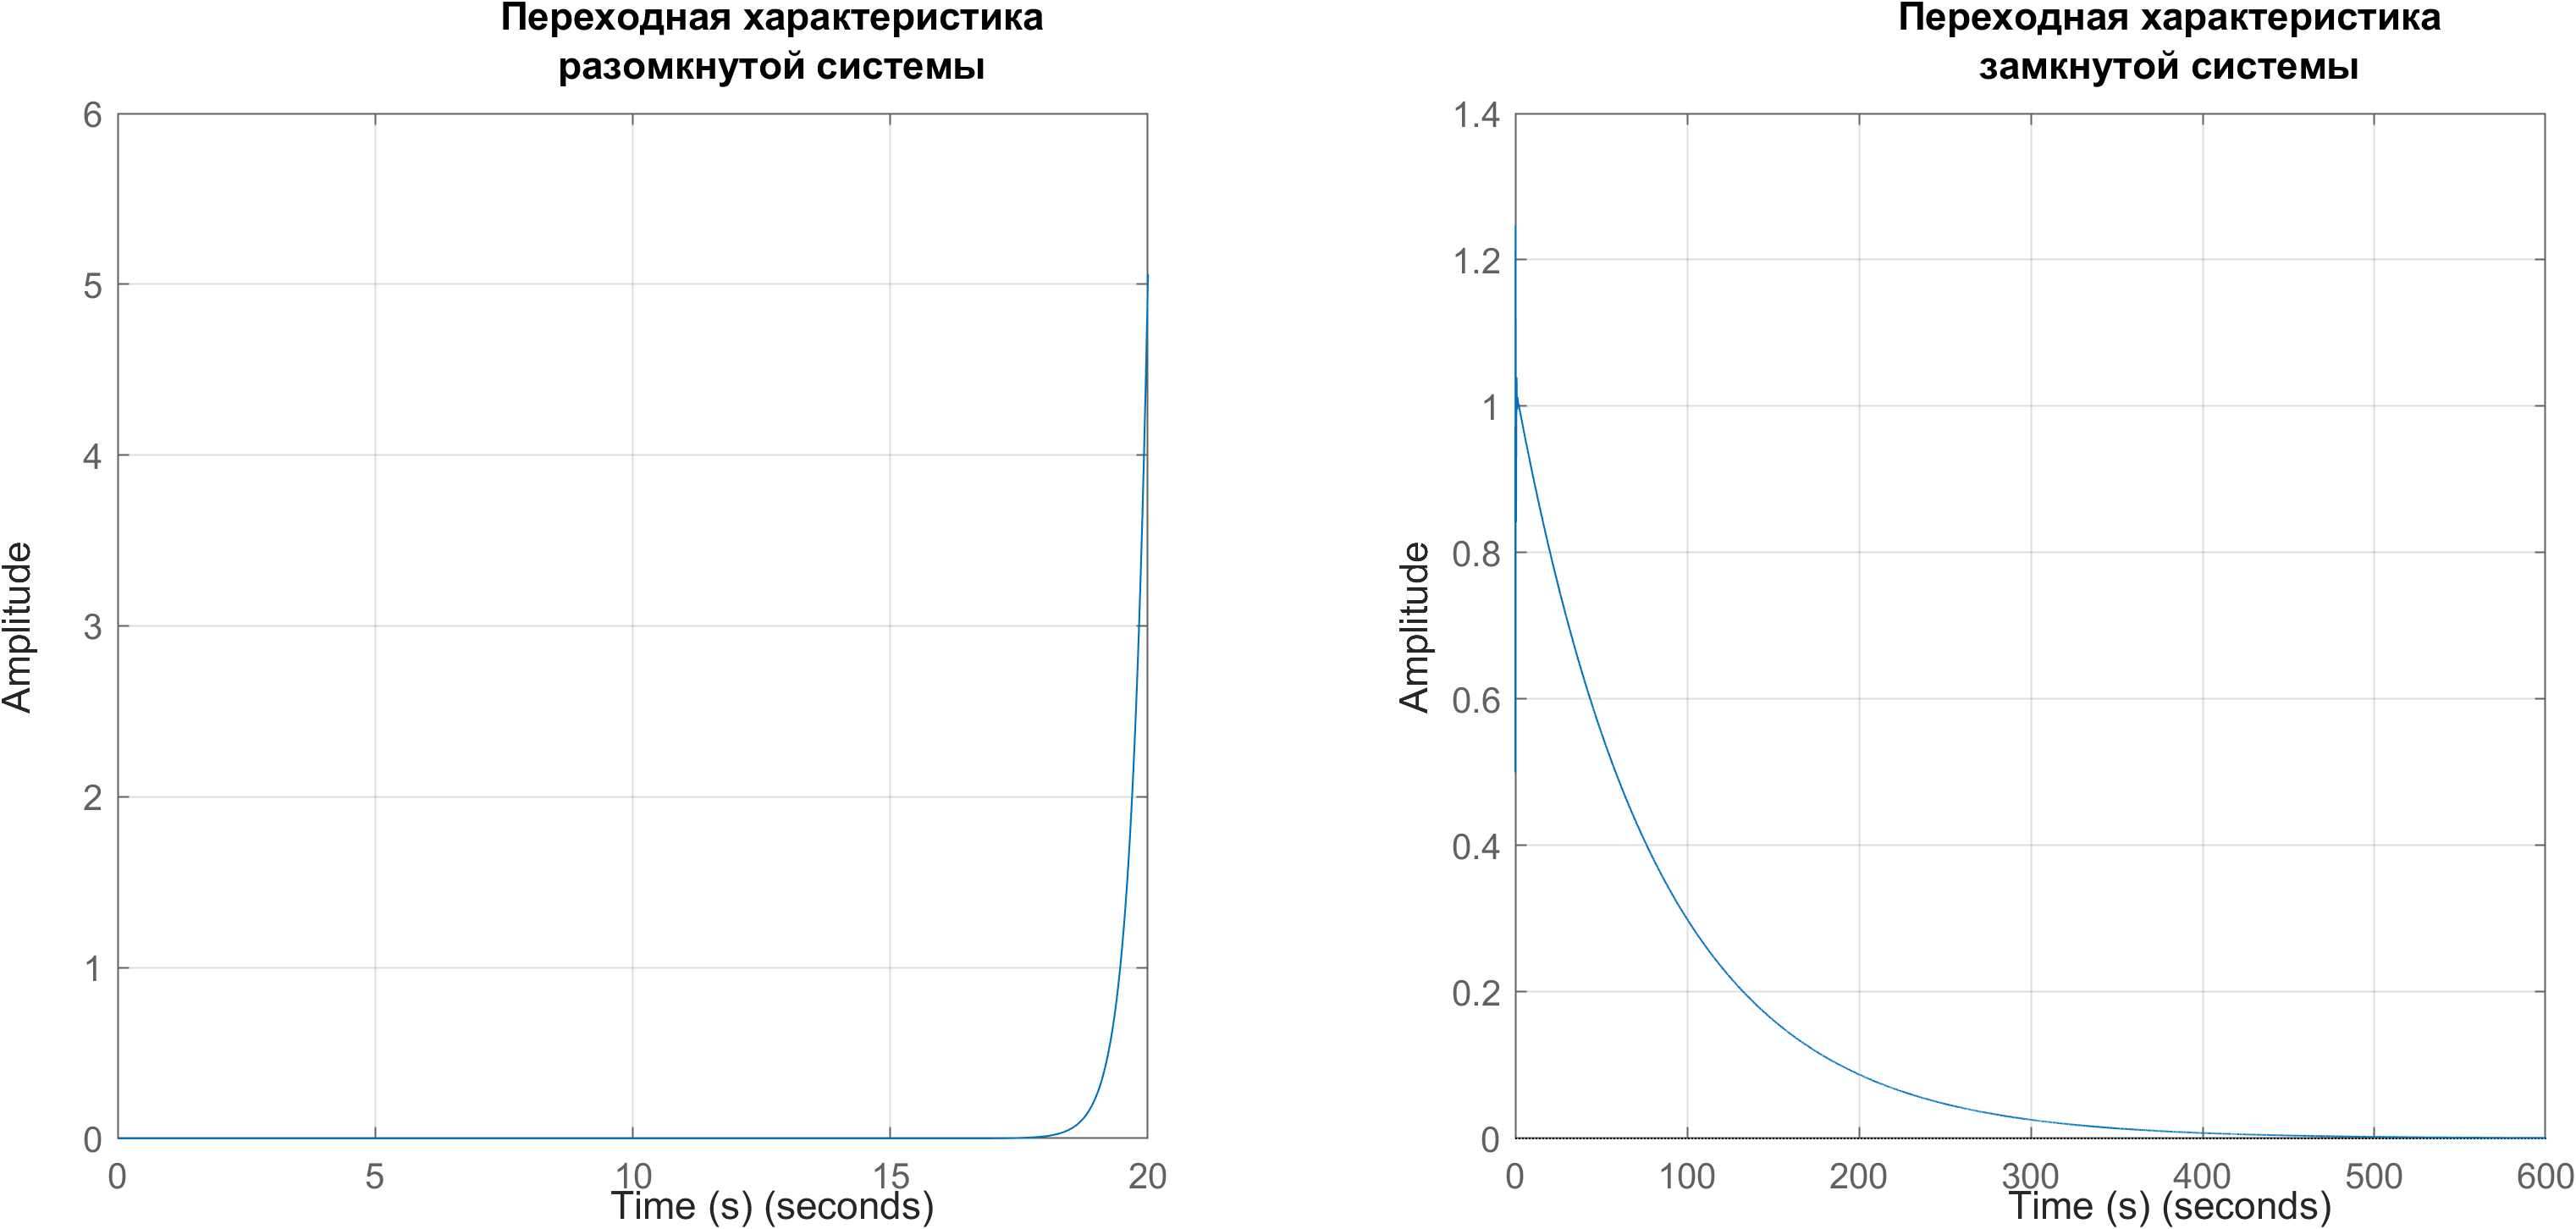
\includegraphics[width=\textwidth]{figs/task_1_obj_3_step.png}
    \caption{Переходные характеристики объекта 3}
    \label{fig:obj3_step}
\end{figure}

\begin{figure}[H]
    \centering
    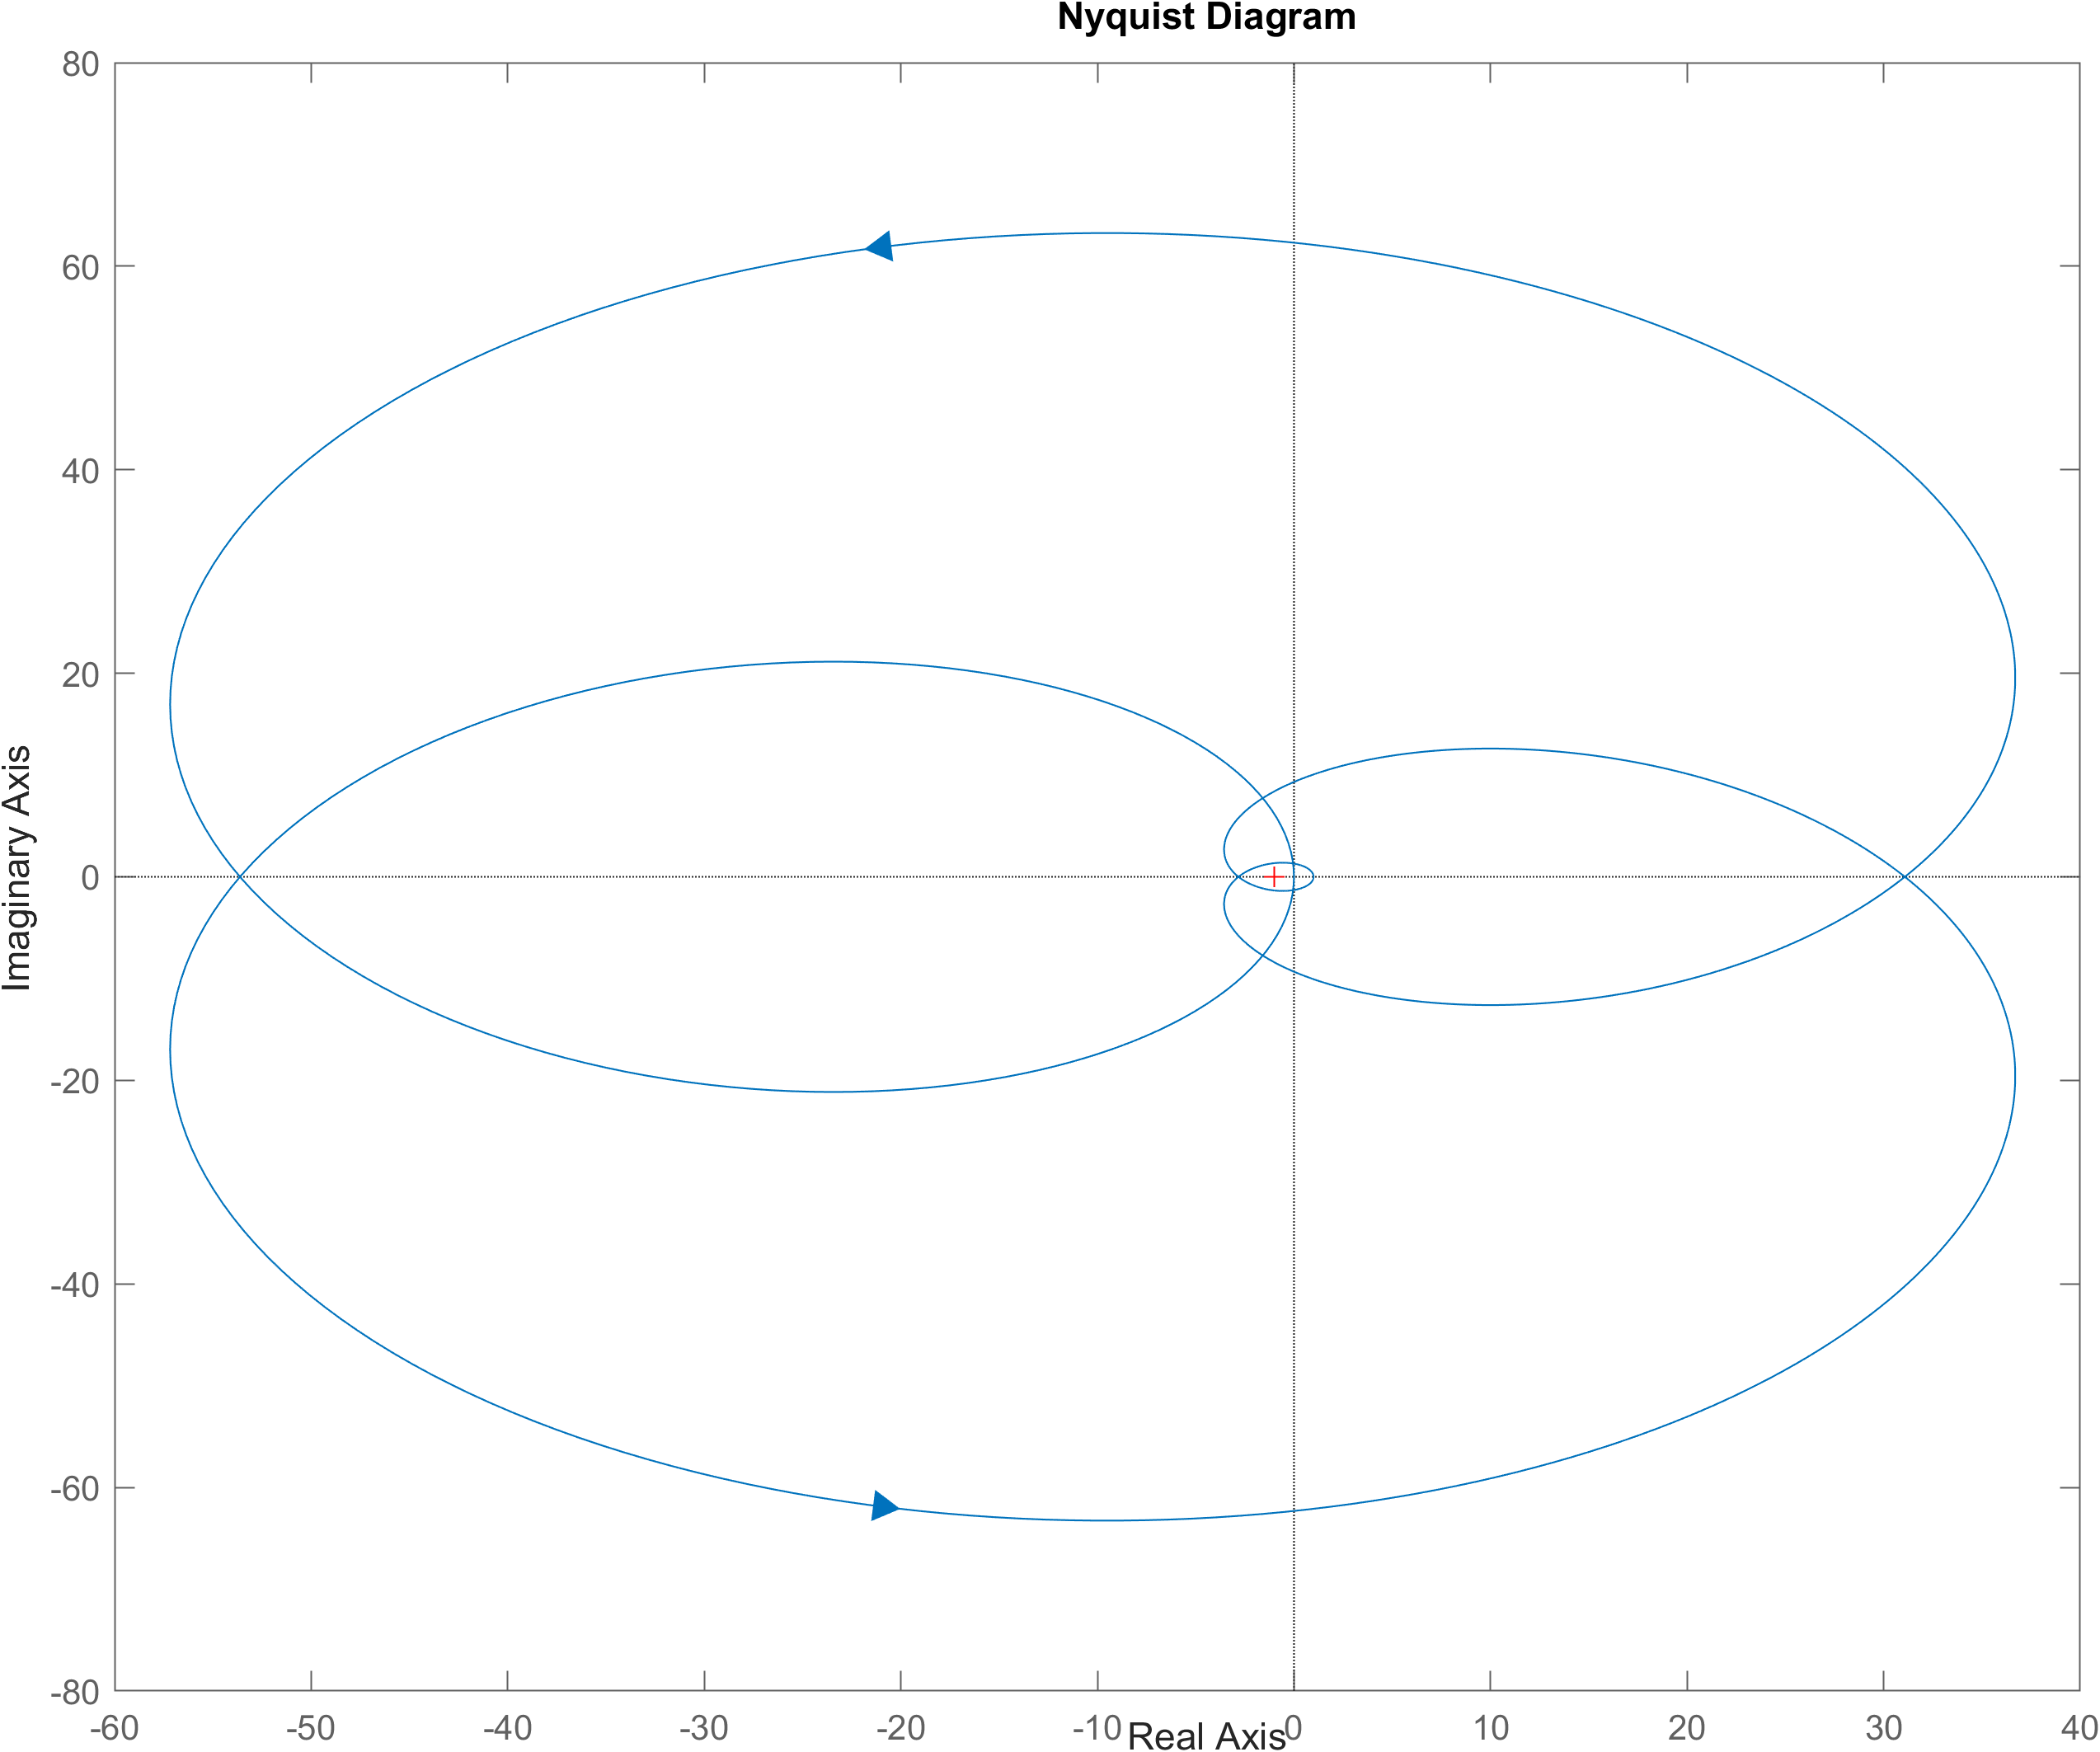
\includegraphics[width=\textwidth]{figs/task_1_obj_3_nyquist.png}
    \caption{Годограф Найквиста объекта 3}
    \label{fig:obj3_nyquist}
\end{figure}

\begin{figure}[H]
    \centering
    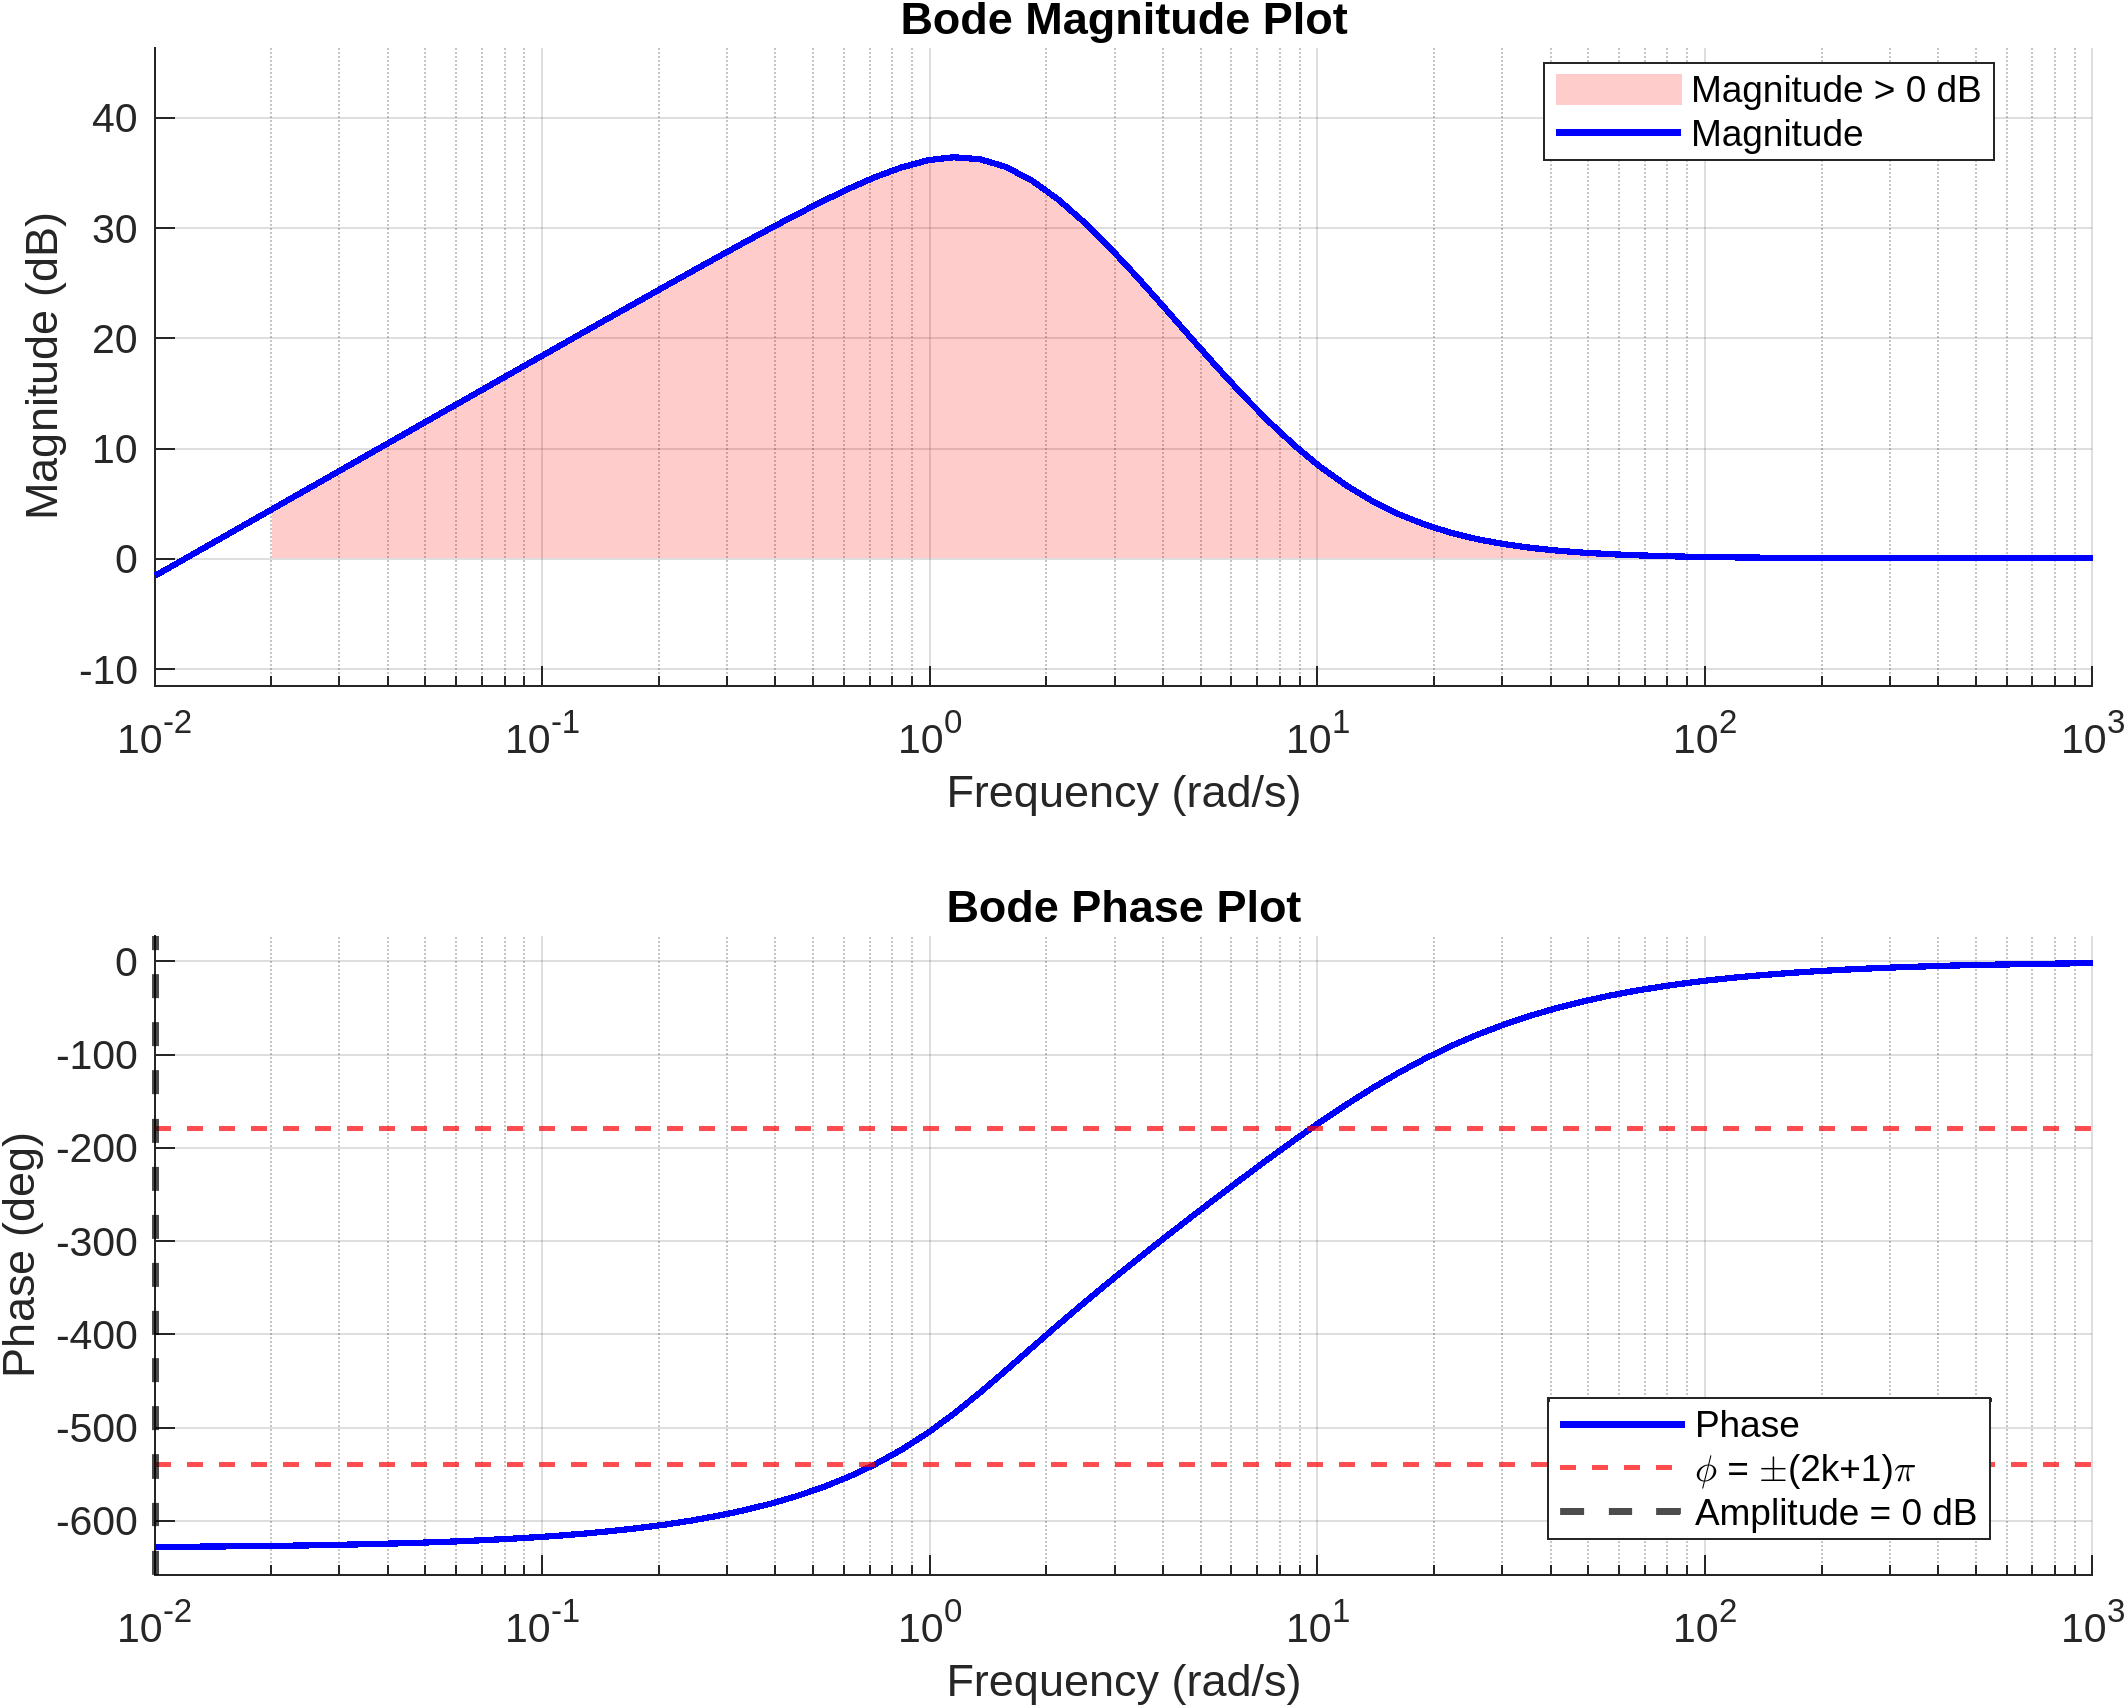
\includegraphics[width=\textwidth]{figs/task_1_obj_3_bode.png}
    \caption{ЛАФЧХ разомкнутой системы объекта 3}
    \label{fig:obj3_bode}
\end{figure}

Переходные характеристики можно увидеть на рисунке \ref{fig:obj3_step},
разомкнутая рассходится, а замкнутая асимптотичесхи сходится. 
Годограф Найквиста можно увидеть на рисунке 
\ref{fig:obj3_nyquist}, как видно, число оборотов против часовой стрелки
вокруг (-1; 0) равняется 4, что соответствует выводам по критерию Найквиста
выше. ЛАФЧХ разомкнутой системы можно увидеть на рисунке \ref{fig:obj3_bode},
воспользовавшись логарифмическим критерием Найквиста, убеждаемся, что 
замкнутая система будет устойчива, так как переходов $2$, и нужно $2$.


\newpage
\section{Коэффициент усиления}

В соответствии с вариантом имеем две ПФ:
\begin{equation*}
    W_1(s)=\frac{s-3}{s^2+2s+6},\quad W_2(s)=\frac{10s^3-13s^2+10s-2}{10s^3+14s^2+5s+0.5}.
\end{equation*}

\begin{table}[H]
    \centering
    \caption{Полюса в задании 2}
    \begin{tabular}{|c|c|}
        \hline
        $W_1(s)$ & $W_2(s)$ \\ \hline
        $-1 + j\sqrt 5$ & $-0.9118$ \\ \hline
        $-1 - j\sqrt 5$ & $-0.3131$ \\ \hline
         ---            & $-0.1752$ \\ \hline
    \end{tabular}
    \label{tab:2poles}
\end{table}

Годографы для них при $k=1$ можно на рисунке \ref{fig:W12_nyquist},
а полюса в таблице \ref{tab:2poles}.
На рисунке этом же рисунке можно увидеть годографы при других $k$. Как видно,
увеличение $k$ увеличивает мастаб годографа равномерно по обоим осям,
то есть просто влияет амплитуду.

% \begin{figure}[H]
%     \centering
%     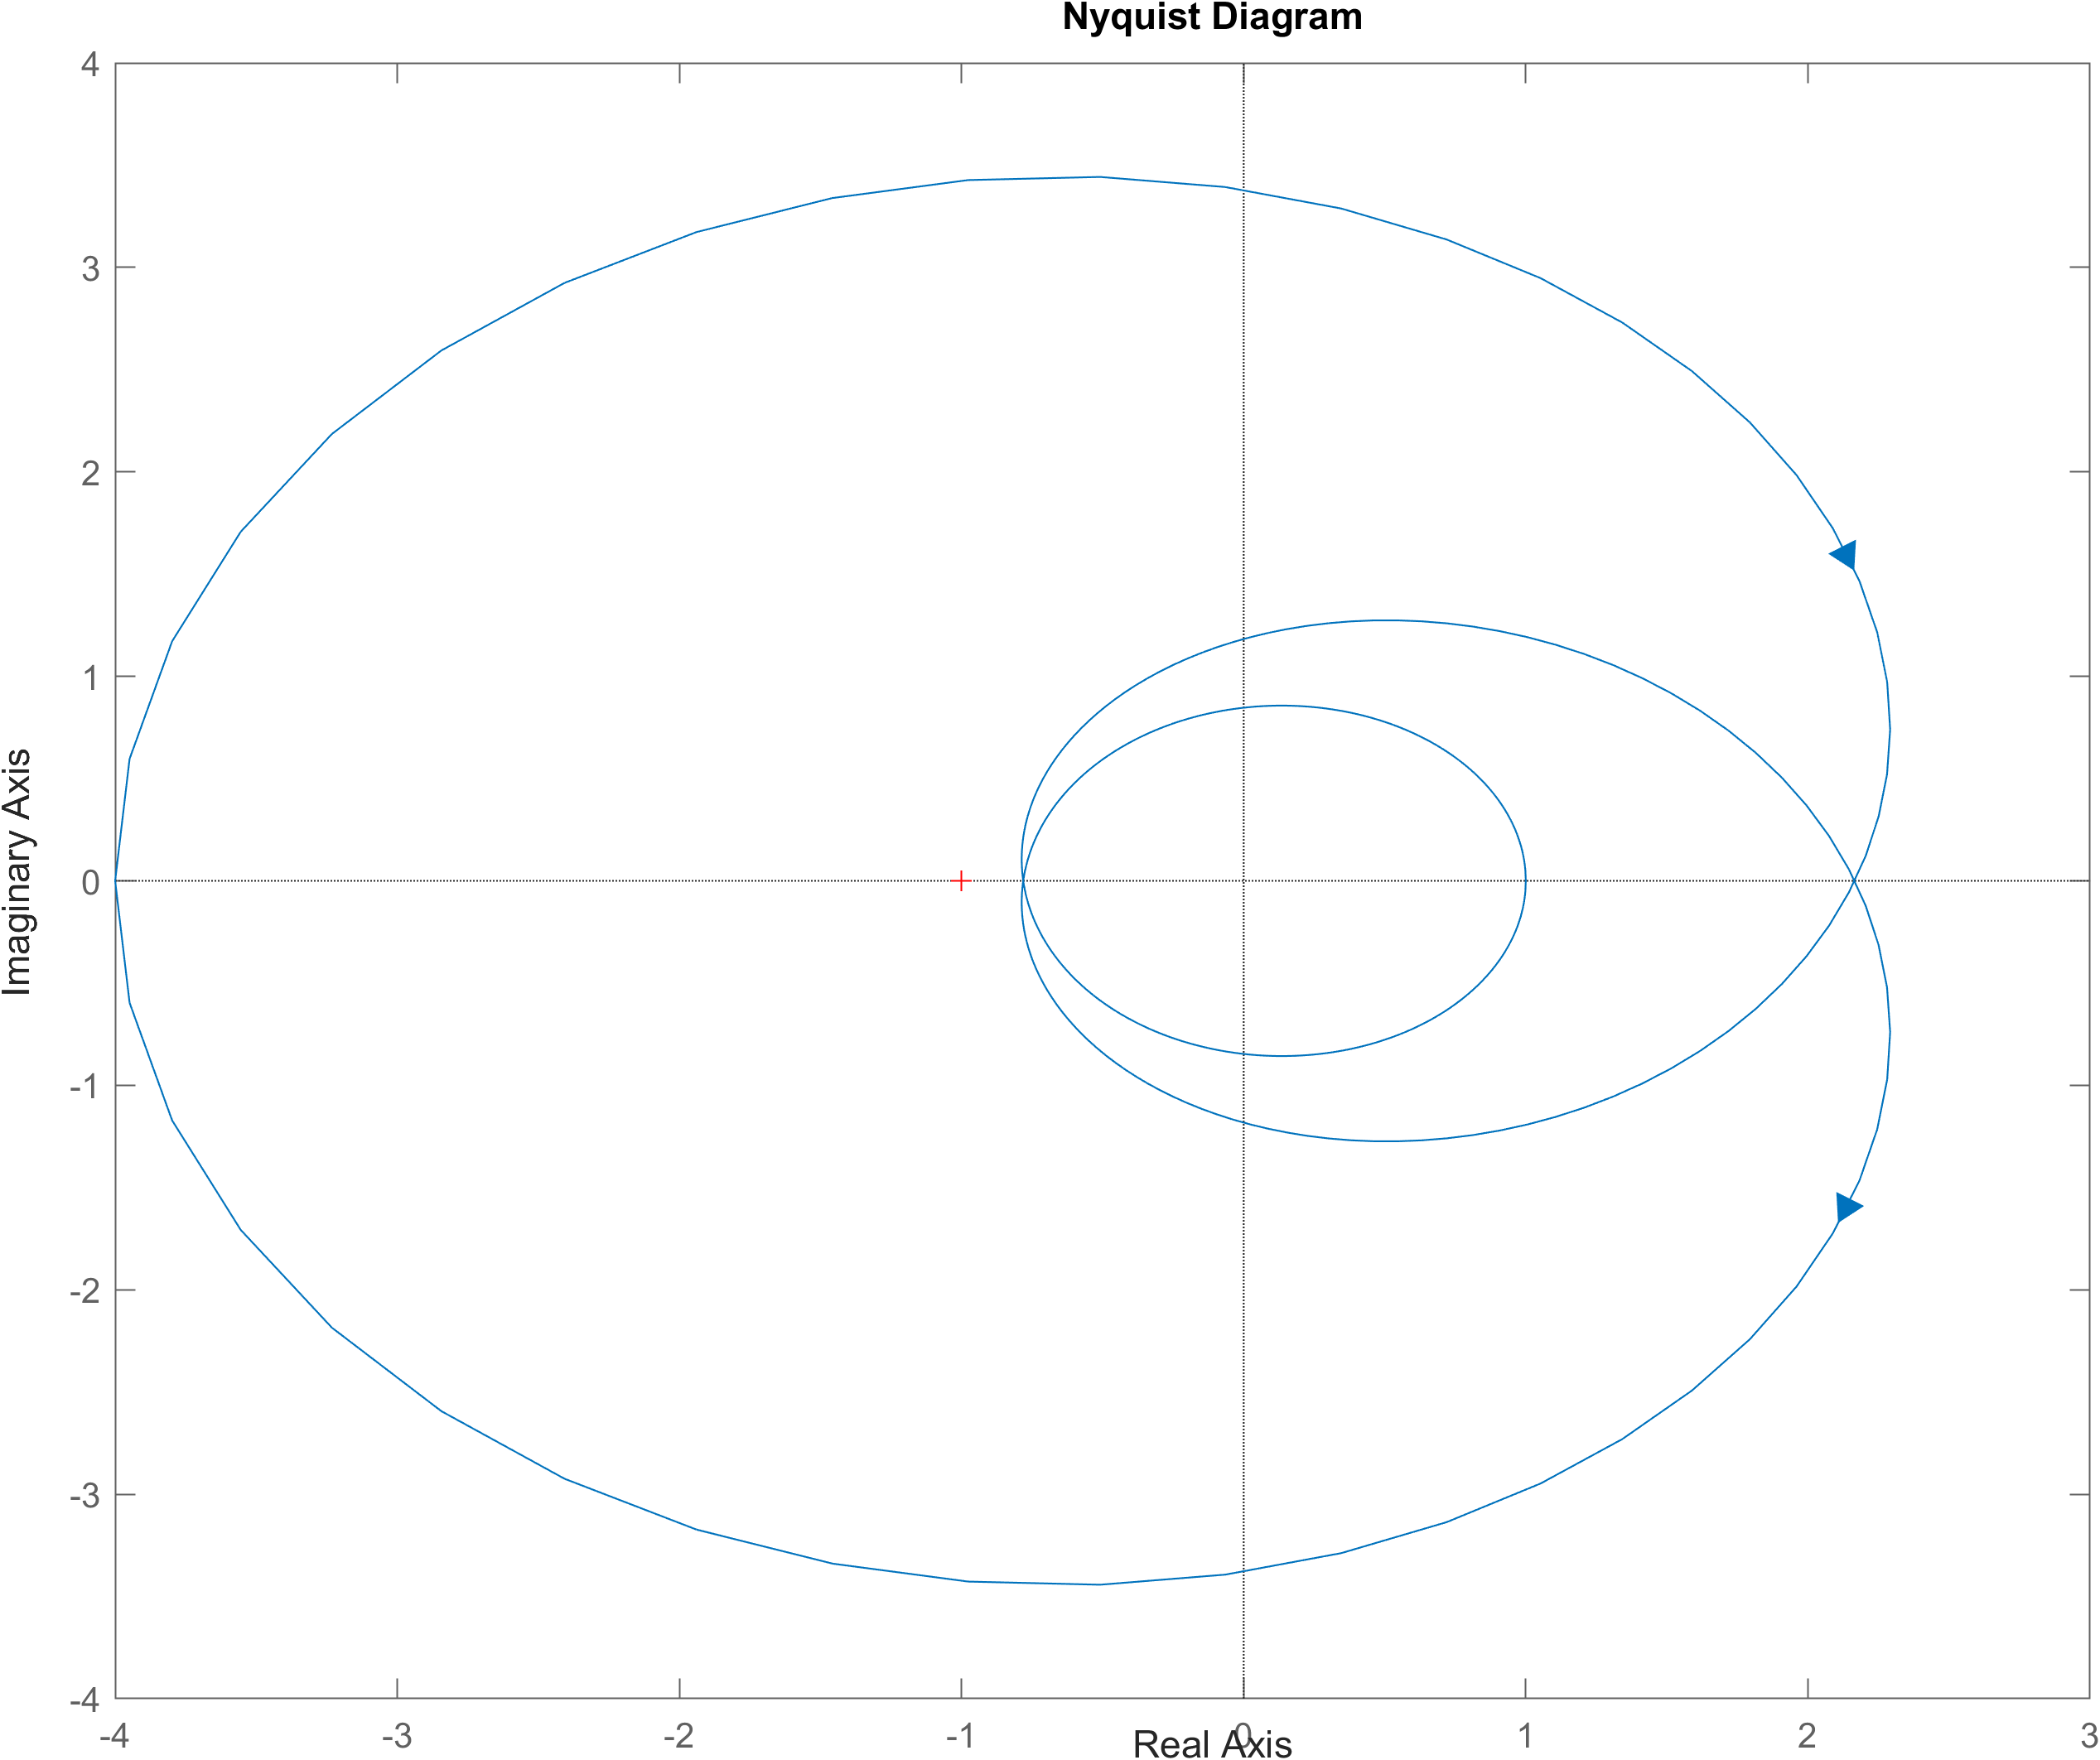
\includegraphics[width=0.9\textwidth]{figs/task_2_2_nyquist.png}
%     \caption{Годограф Найквиста для $W_2(s)$}
%     \label{fig:W2_nyquist}
% \end{figure}

\begin{figure}[H]
    \centering
    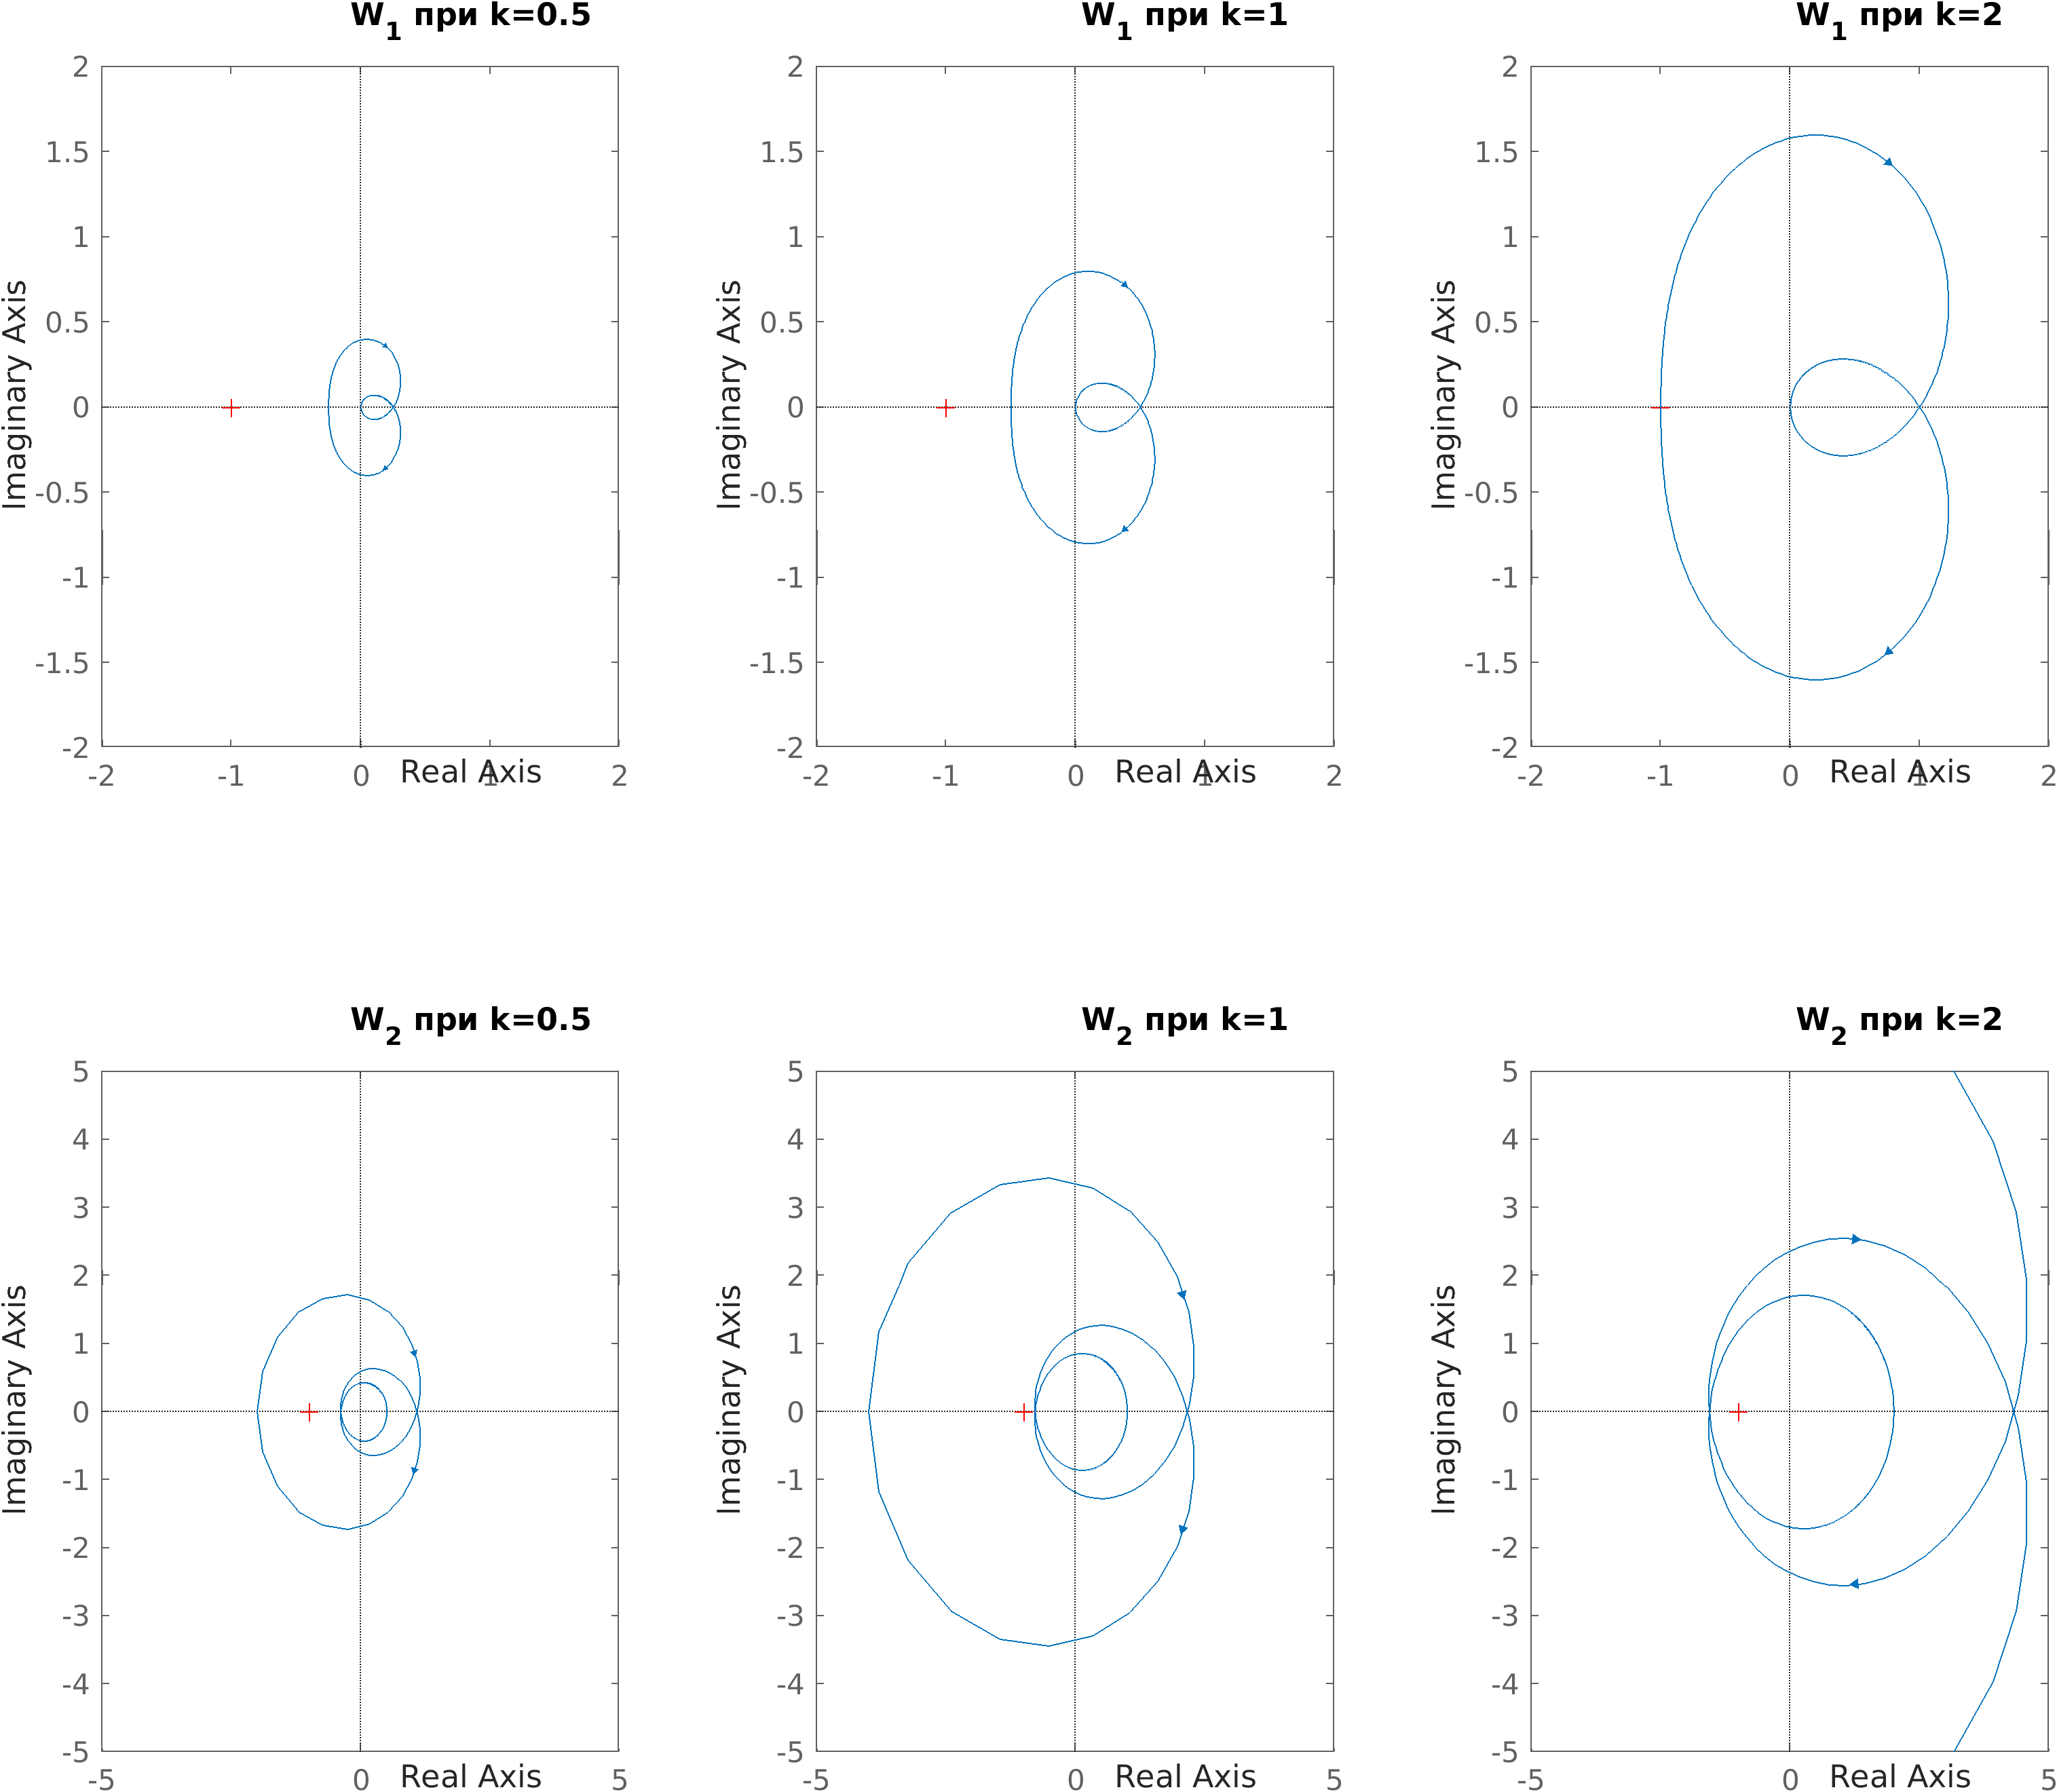
\includegraphics[width=\textwidth]{figs/task_2_ks_nyaquist.png}
    \caption{Годографы Найквиста при разных $k$}
    \label{fig:W12_nyquist}
\end{figure}

\subsection{Первая ПФ}
Рассмотрим первую ПФ:
\begin{equation*}
    \begin{split}
    W_1(j\omega)=\frac{j\omega-3}{j\omega^2+2j\omega+6}
    =\frac{-3+j\omega}{(1+j(\omega+\sqrt{5}))(1+j(\omega-\sqrt{5}))}=\\
    =\sqrt{\frac{9+\omega^2}{(1+(\omega-\sqrt{5})^2)(1+(\omega+\sqrt{5})^2)}}
    \exp \left( j\left[ \text{atan2}(\omega;-3) - \text{atan2}(\omega+\sqrt 5;1) - \text{atan2}(\omega-\sqrt 5;1) \right] \right),
    \end{split}
\end{equation*}
тогда, если 
\begin{equation*}
    (1+(\omega-\sqrt{5})^2)(1+(\omega+\sqrt{5})^2)=\omega^4-8\omega^2+36,
\end{equation*}
то амплитуда и фаза равны
\begin{equation*}
    A(\omega)=\sqrt{\frac{9+\omega^2}{\omega^4-8\omega^2+36}},
    \quad \varphi(\omega)=\text{atan2}(\omega;-3) - \text{atan2}(\omega+\sqrt 5;1) - \text{atan2}(\omega-\sqrt 5;1).
\end{equation*}
Заметим, что при $\omega=0$ фаза равняется $\pi$, как видно по рисунку \ref{fig:W12_nyquist}
других решений $\varphi(\omega)=\pm\pi$ нет. Теперь можем найти амплитуду запаса:
\begin{equation*}
    A_\text{з}=\frac{1}{A(0)}=2=k_{max}.
\end{equation*}
Значит при $k\geq 2$ замкнутая система будет нестойчива, при $k<2$ система будет
асимптотически устойчива. Чтобы это проверить получим переходную характеристику
в MATLAB для этих промежутков, результат можно увидеть на рисунке \ref{fig:W1_step},
выводы подтвердились.

\begin{figure}[H]
    \centering
    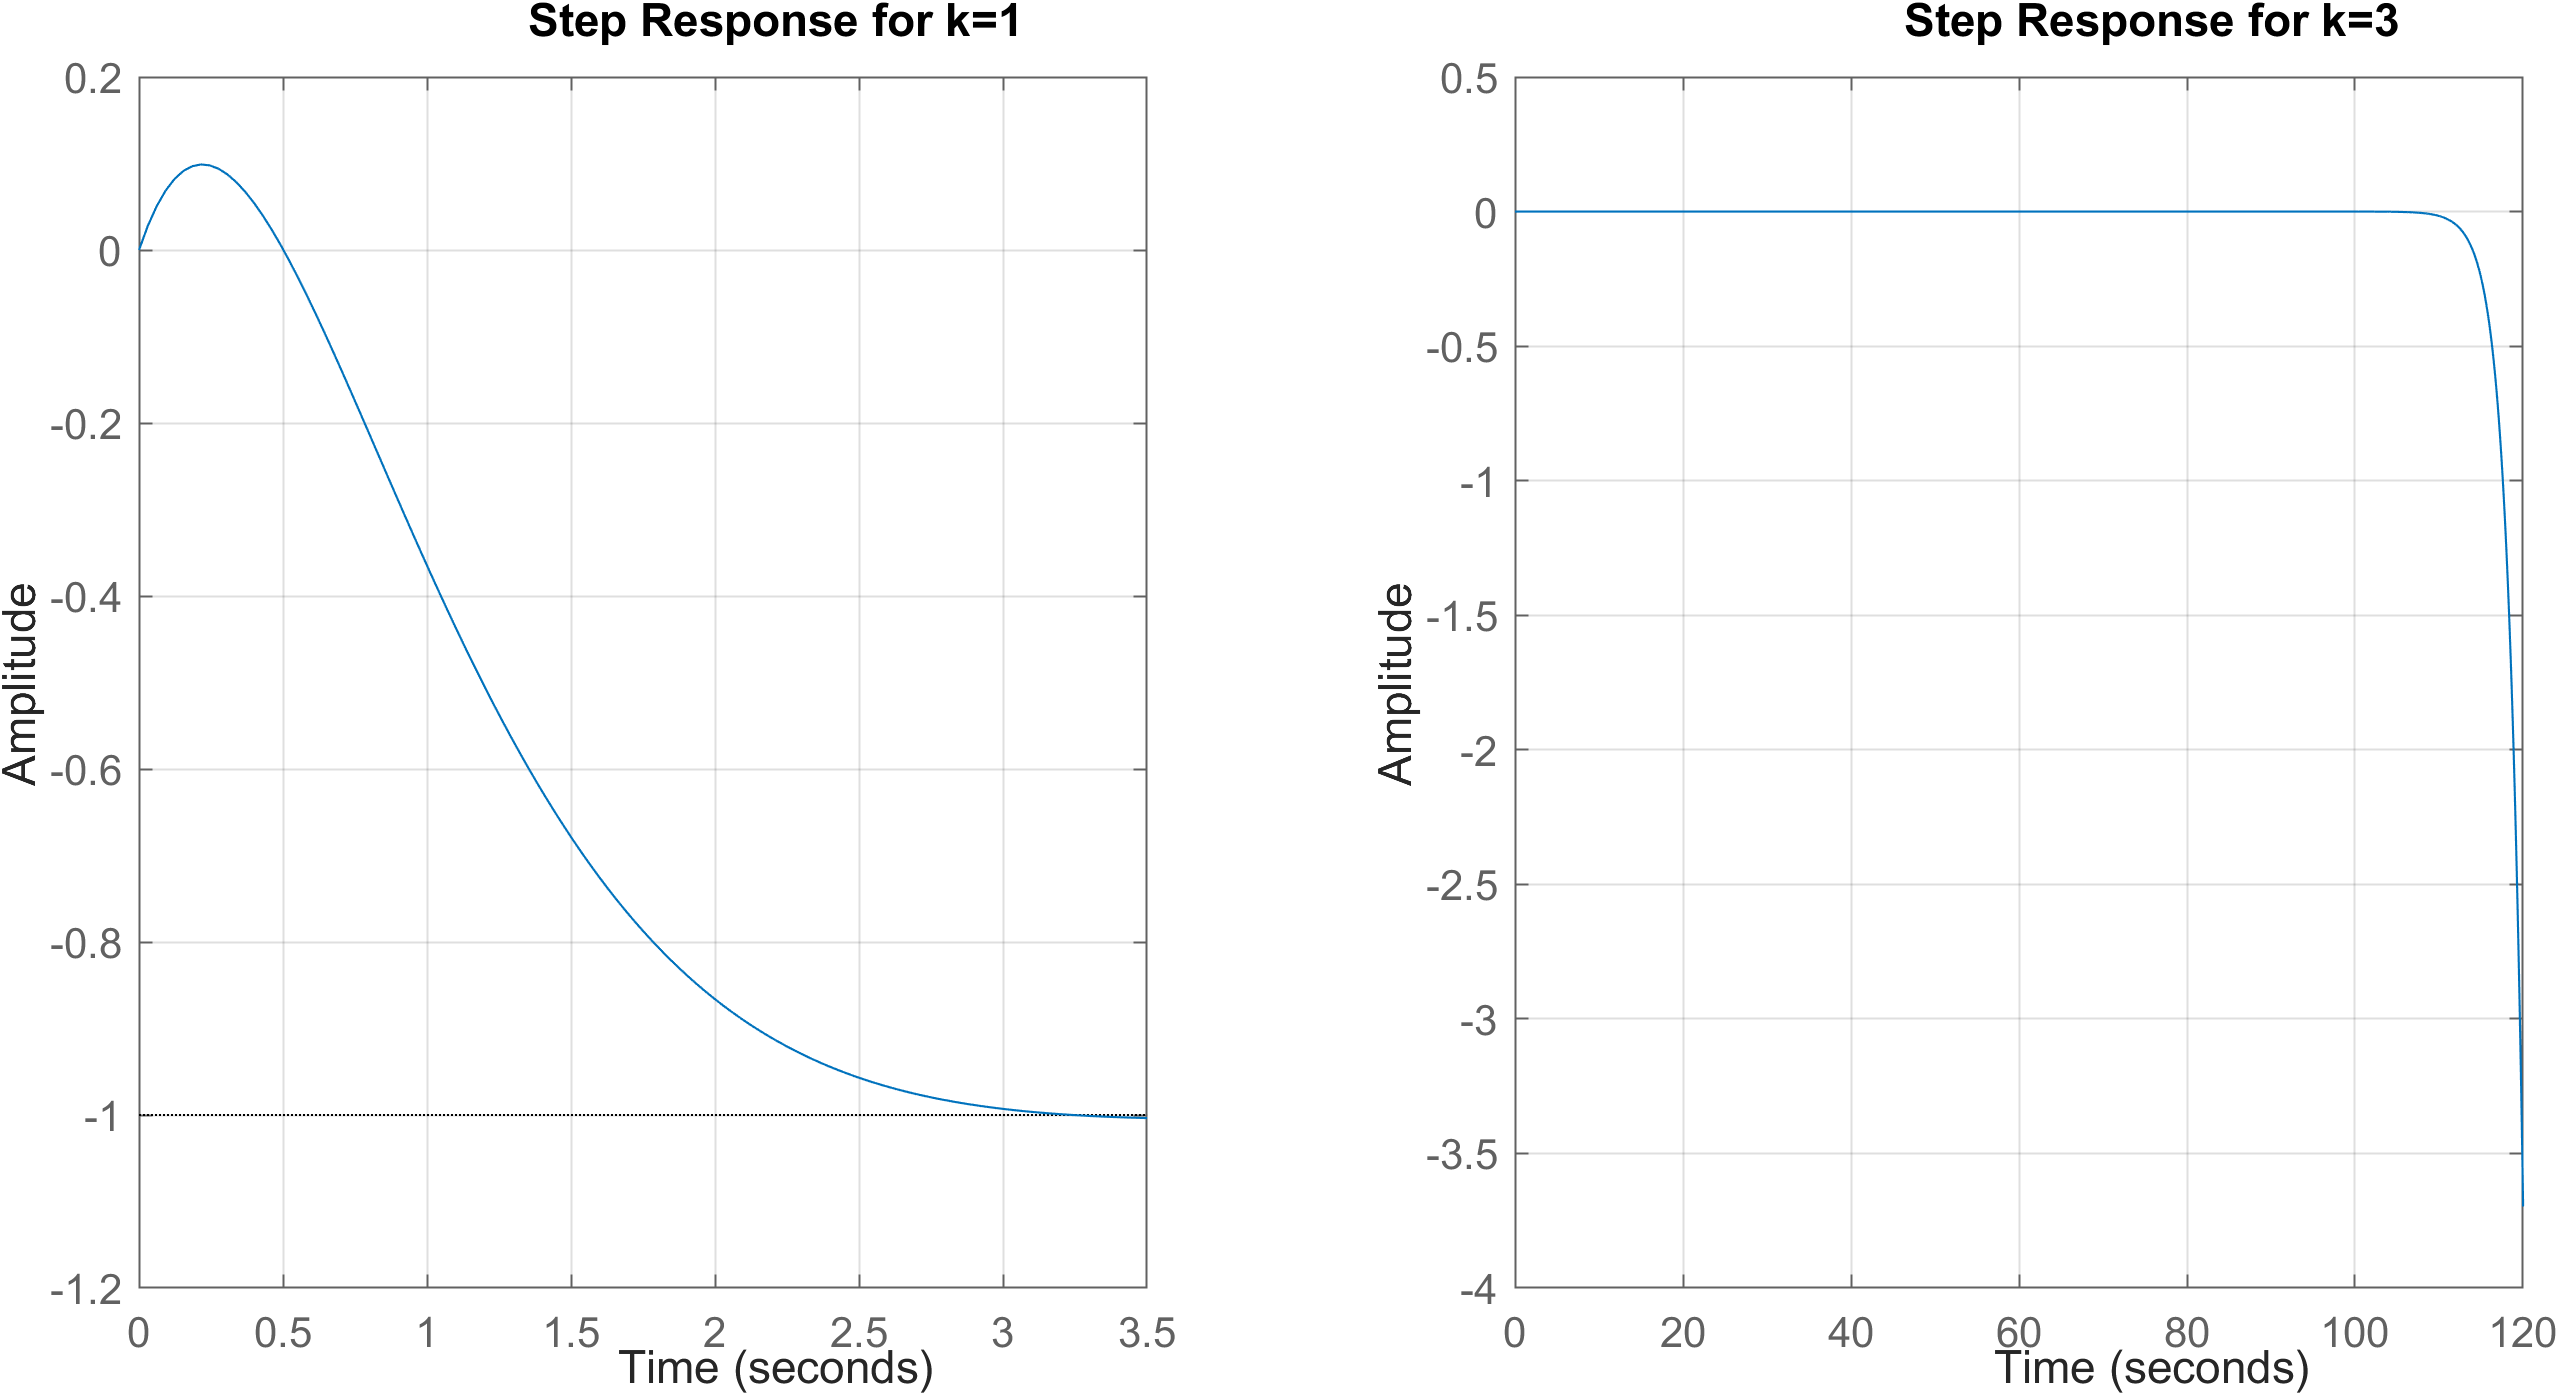
\includegraphics[width=\textwidth]{figs/task_2_W1_ksteps.png}
    \caption{Переходные характеристики замкнутой первой ПФ для различных $k$}
    \label{fig:W1_step}
\end{figure}

\newpage
\subsection{Вторая ПФ}

Рассмотрим вторую ПФ:
\begin{equation*}
    \begin{split}
        W_2(j\omega) & \approx
        \frac{(-0.51 + j(\omega + 0.67))(-0.51 + j(\omega - 0.67))(-0.28 + j\omega)}
             {(0.91 + j\omega)(0.31 + j\omega)(0.18 + j\omega)} \\
        & = 
        \frac{
            \sqrt{0.26 + (\omega + 0.67)^2} \sqrt{0.26 + (\omega - 0.67)^2} \sqrt{0.08 + \omega^2}
        }{
            \sqrt{0.83 + \omega^2} \sqrt{0.10 + \omega^2} \sqrt{0.03 + \omega^2}
        } \\
        & \quad \times 
        \exp\Big[j(
            \text{atan2}(\omega + 0.67, -0.51) 
            + \text{atan2}(\omega - 0.67, -0.51) 
            + \text{atan2}(\omega, -0.28) \\
        & \quad \quad \quad
            - \text{atan2}(\omega, 0.91) 
            - \text{atan2}(\omega, 0.31) 
            - \text{atan2}(\omega, 0.18))
        \Big].
    \end{split}
\end{equation*}
Тогда амплитуда и фаза равны
\begin{equation*}
    A(\omega)=\frac{
            \sqrt{0.26 + (\omega + 0.67)^2} \sqrt{0.26 + (\omega - 0.67)^2} \sqrt{0.08 + \omega^2}
        }{
            \sqrt{0.83 + \omega^2} \sqrt{0.10 + \omega^2} \sqrt{0.03 + \omega^2}
        },
\end{equation*}
\begin{equation*}
\begin{split}
    \varphi(\omega)=&\text{atan2}(\omega + 0.67, -0.51) 
    + \text{atan2}(\omega - 0.67, -0.51) 
    + \text{atan2}(\omega, -0.28)\\
    &- \text{atan2}(\omega, 0.91) 
    - \text{atan2}(\omega, 0.31) 
    - \text{atan2}(\omega, 0.18).
\end{split}
\end{equation*}
Заметим, что при $\omega=0$ фаза равняется $5\pi$, а так же при около $\omega\approx 0.9389$
(найденно численно)  фаза равняется $\pi$, как видно по рисунку \ref{fig:W12_nyquist}
 - это единсвенные решения для положительных частот уравнения $\varphi(\omega)=\pm(2n\pi+1),\ n\in\{0, 1, 2\dots\}$.

 \begin{figure}[H]
    \centering
    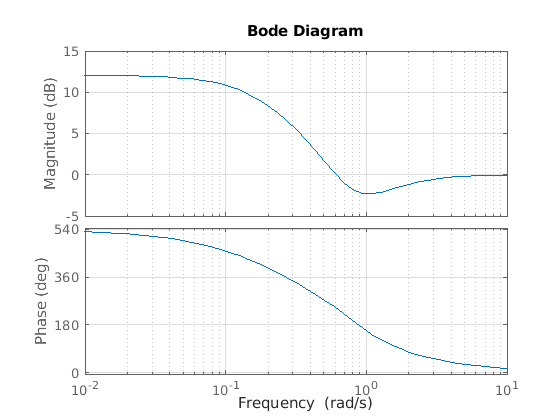
\includegraphics[width=0.7\textwidth]{figs/task_2_W2_bode.png}
    \caption{ЛАФЧХ второй ПФ}
    \label{fig:2W2_bode}
\end{figure}

Как мы можем видить по полюсам второй ПФ в таблице \ref{tab:2poles},
разомкнутая система асимптотически устойчива, значит достаточно исключить 
закручивания по часовой стрелке вокруг (-1, 0), чтобы закнутая была устойчива.
Посмотрим на ЛАФЧХ второй ПФ на рисунке \ref{fig:2W2_bode}, как видно начинаем
с максимальной амплитудой и фазой $5\pi$ - одно из найденных решений, и если снова
посмотреть на годограф на рисунке \ref{fig:W12_nyquist}, то именно этот начальный и самый
большой закрут нужно исключить. Найдем
амплитуду запаса:
\begin{equation*}
    A_\text{з}=\frac{1}{A(0)}\approx 0.25=k_{max}.
\end{equation*}
Значит при $k\geq 0.25$ замкнутая система будет нестойчива, при $k<0.25$ система будет
устойчива. Чтобы это проверить получим переходную характеристику
в MATLAB для этих промежутков, результат можно увидеть на рисунке \ref{fig:W2_step},
выводы подтвердились.

\begin{figure}[H]
    \centering
    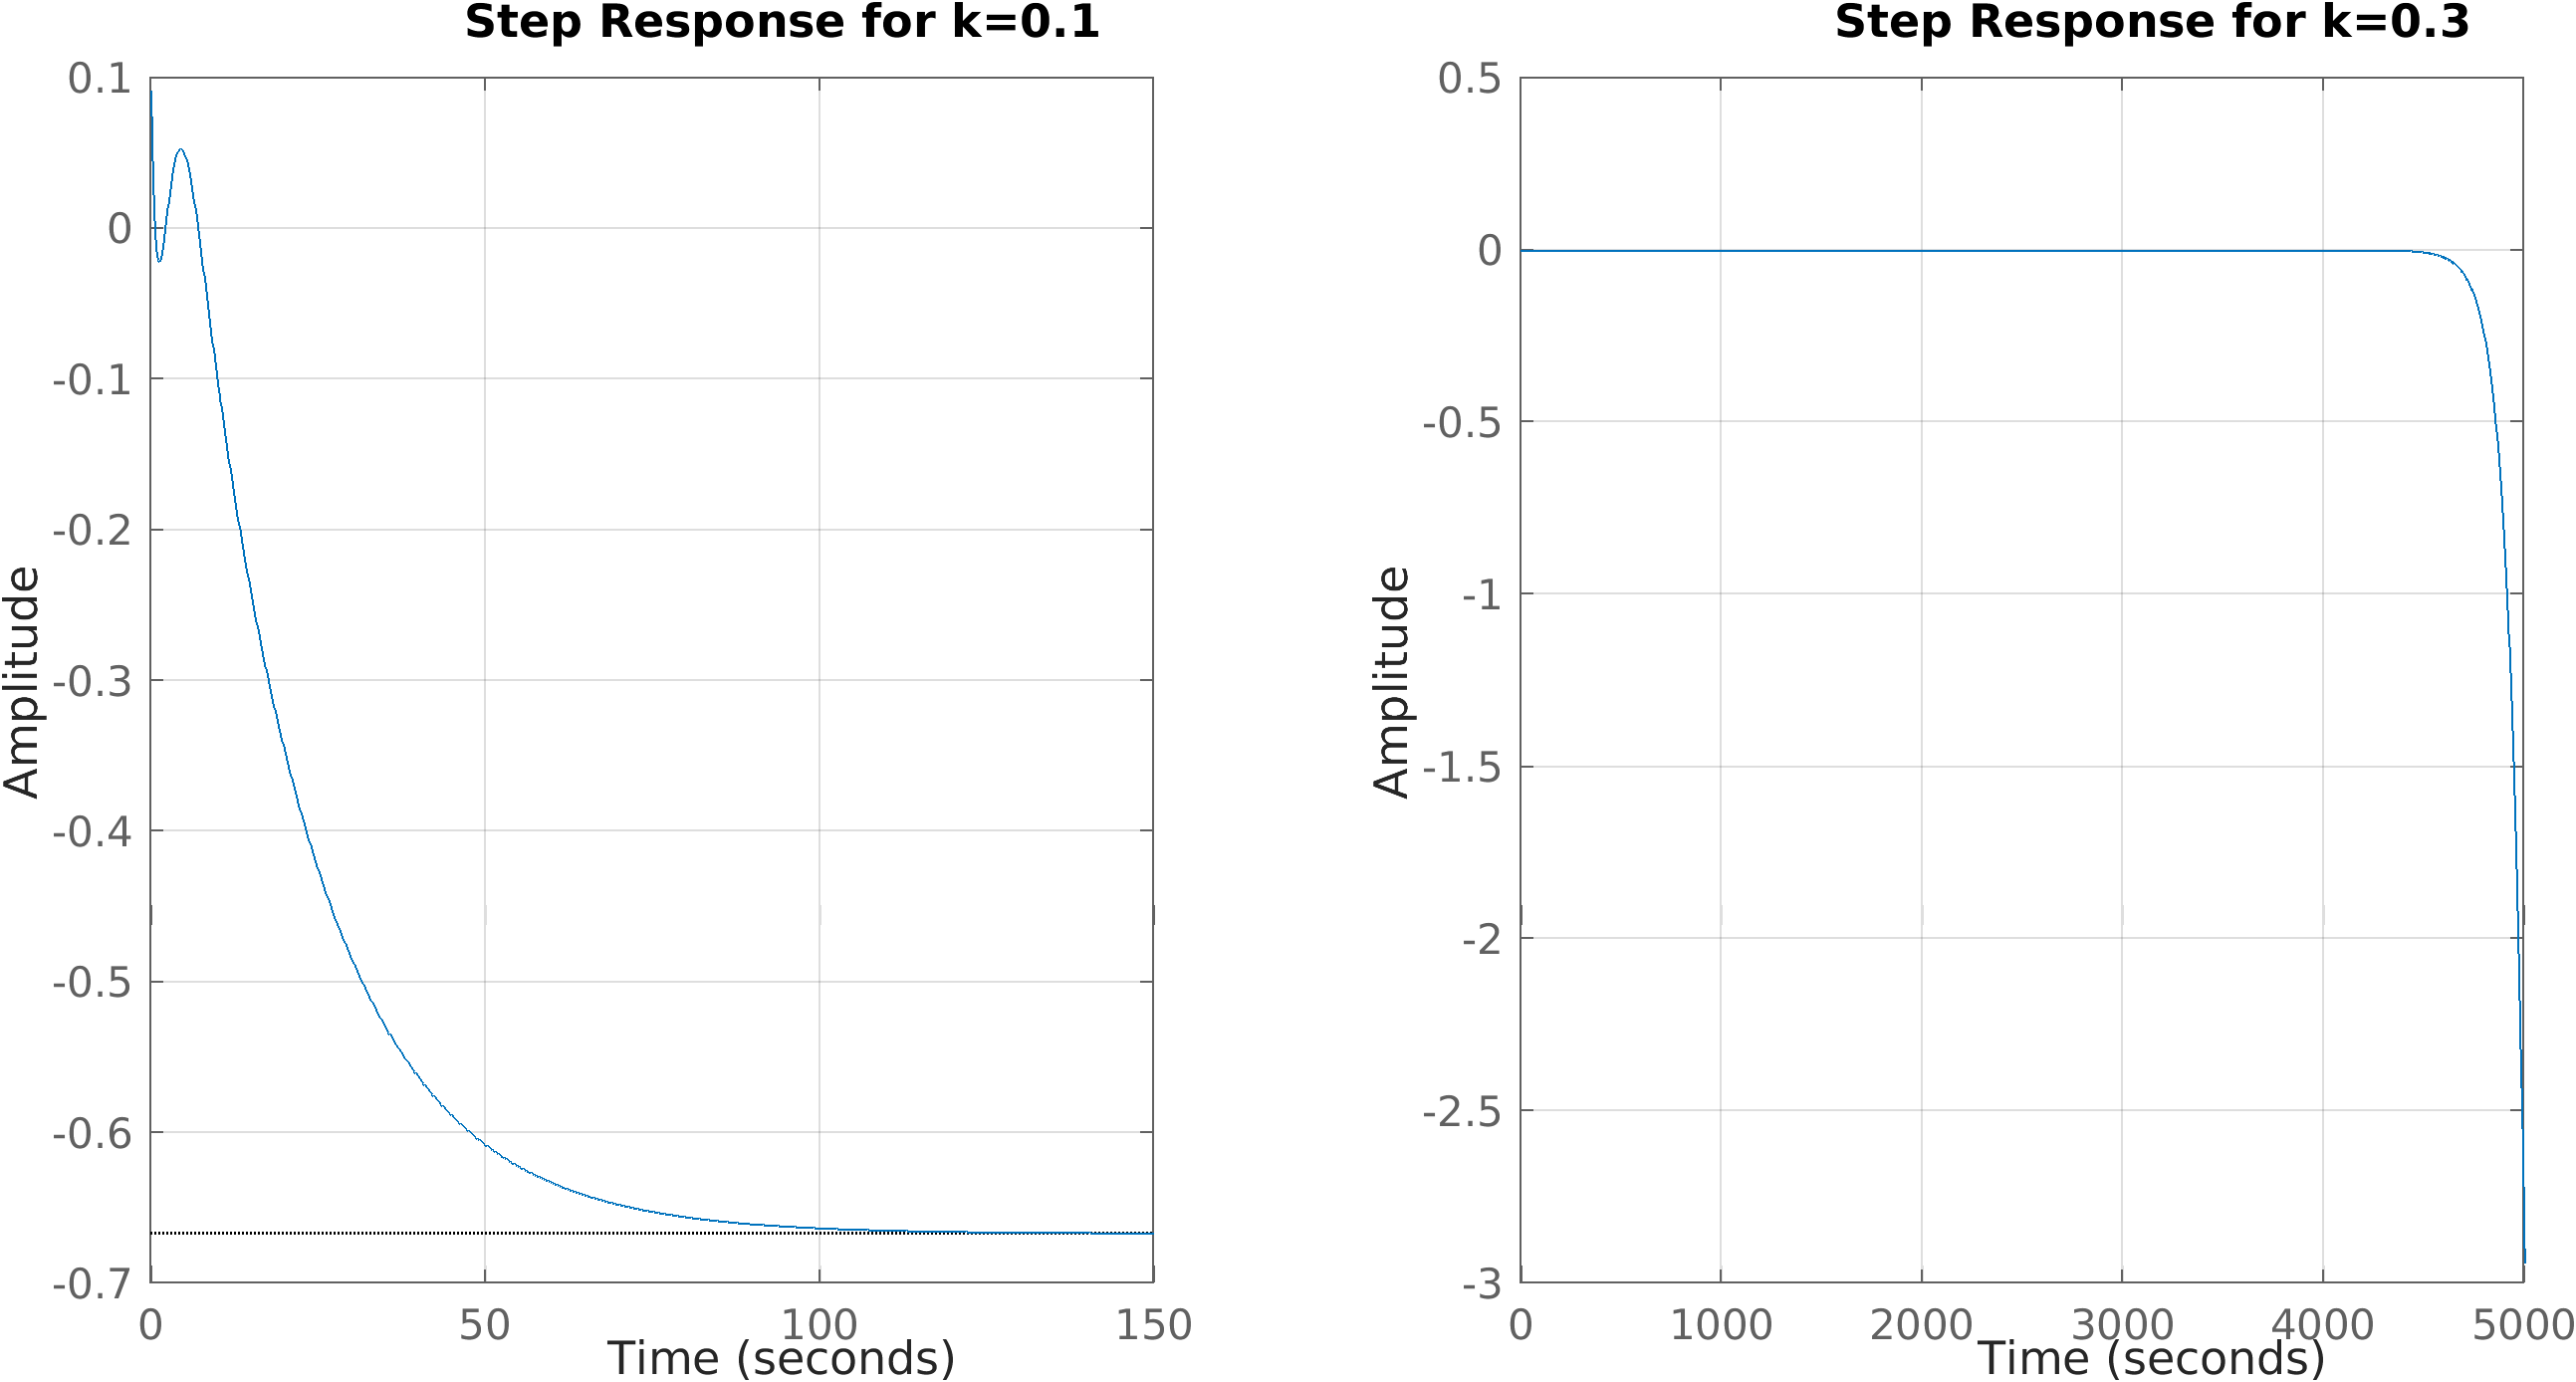
\includegraphics[width=\textwidth]{figs/task_2_W2_ksteps.png}
    \caption{Переходные характеристики замкнутой второй ПФ для различных $k$}
    \label{fig:W2_step}
\end{figure}


\section{Запаздывание}

Согласно варианту имеем
\begin{equation*}
    W_3(s)=\frac{7s+5}{s^2+4s},\quad W_4(s)=\frac{20s^2+1.6s+2}{10s^3-10s^2-0.1s+0.1}.
\end{equation*}
Их полюса можно увидеть в таблице \ref{tab:polesW34}. Как видно, разомкнутая 
$W_3$ асимптотически устойчива, а разомкнутая $W_4$ неустойчива.
Годографы можно увидеть на рисунке \ref{fig:W34_nyquist} для значений
$\tau\in\{0, 0.05, 0.5\}$. Как видно, увеличение $\tau$ закручивает
годограф по часовой стрелке. 

\begin{table}[H]
    \centering
    \caption{Полюса разомкнутых $W_3$ и $W_4$}
    \begin{tabular}{|c|c|}
    \hline
    Полюса $W_3$ & Полюса $W_4$        \\ \hline
        $-4$ & $1$ \\ \hline
        $0$ & $0.1$ \\ \hline
        --- & $-0.1$ \\ \hline
    \end{tabular}
    \label{tab:polesW34}
\end{table}

\subsection{Третья ПФ}
Посмотрим на годограф третьей ПФ, при закручивании
точка (-1; 0) будет охвачиваться по часовой стрелке, значит замкнутая 
может стать неустойчивой.
Рассмотрим ПФ:
\begin{equation*}
    W_3(j\omega)=\frac{7j\omega+5}{-\omega^2+4j\omega}
    =\frac{\sqrt{25+49\omega^2}}{\sqrt{\omega^4+16\omega^2}}\exp \left( j \left[ \text{atan2}(7\omega;5) - \text{atan2}(4\omega;-\omega^2) \right] \right).
\end{equation*}
\begin{figure}[H]
    \centering
    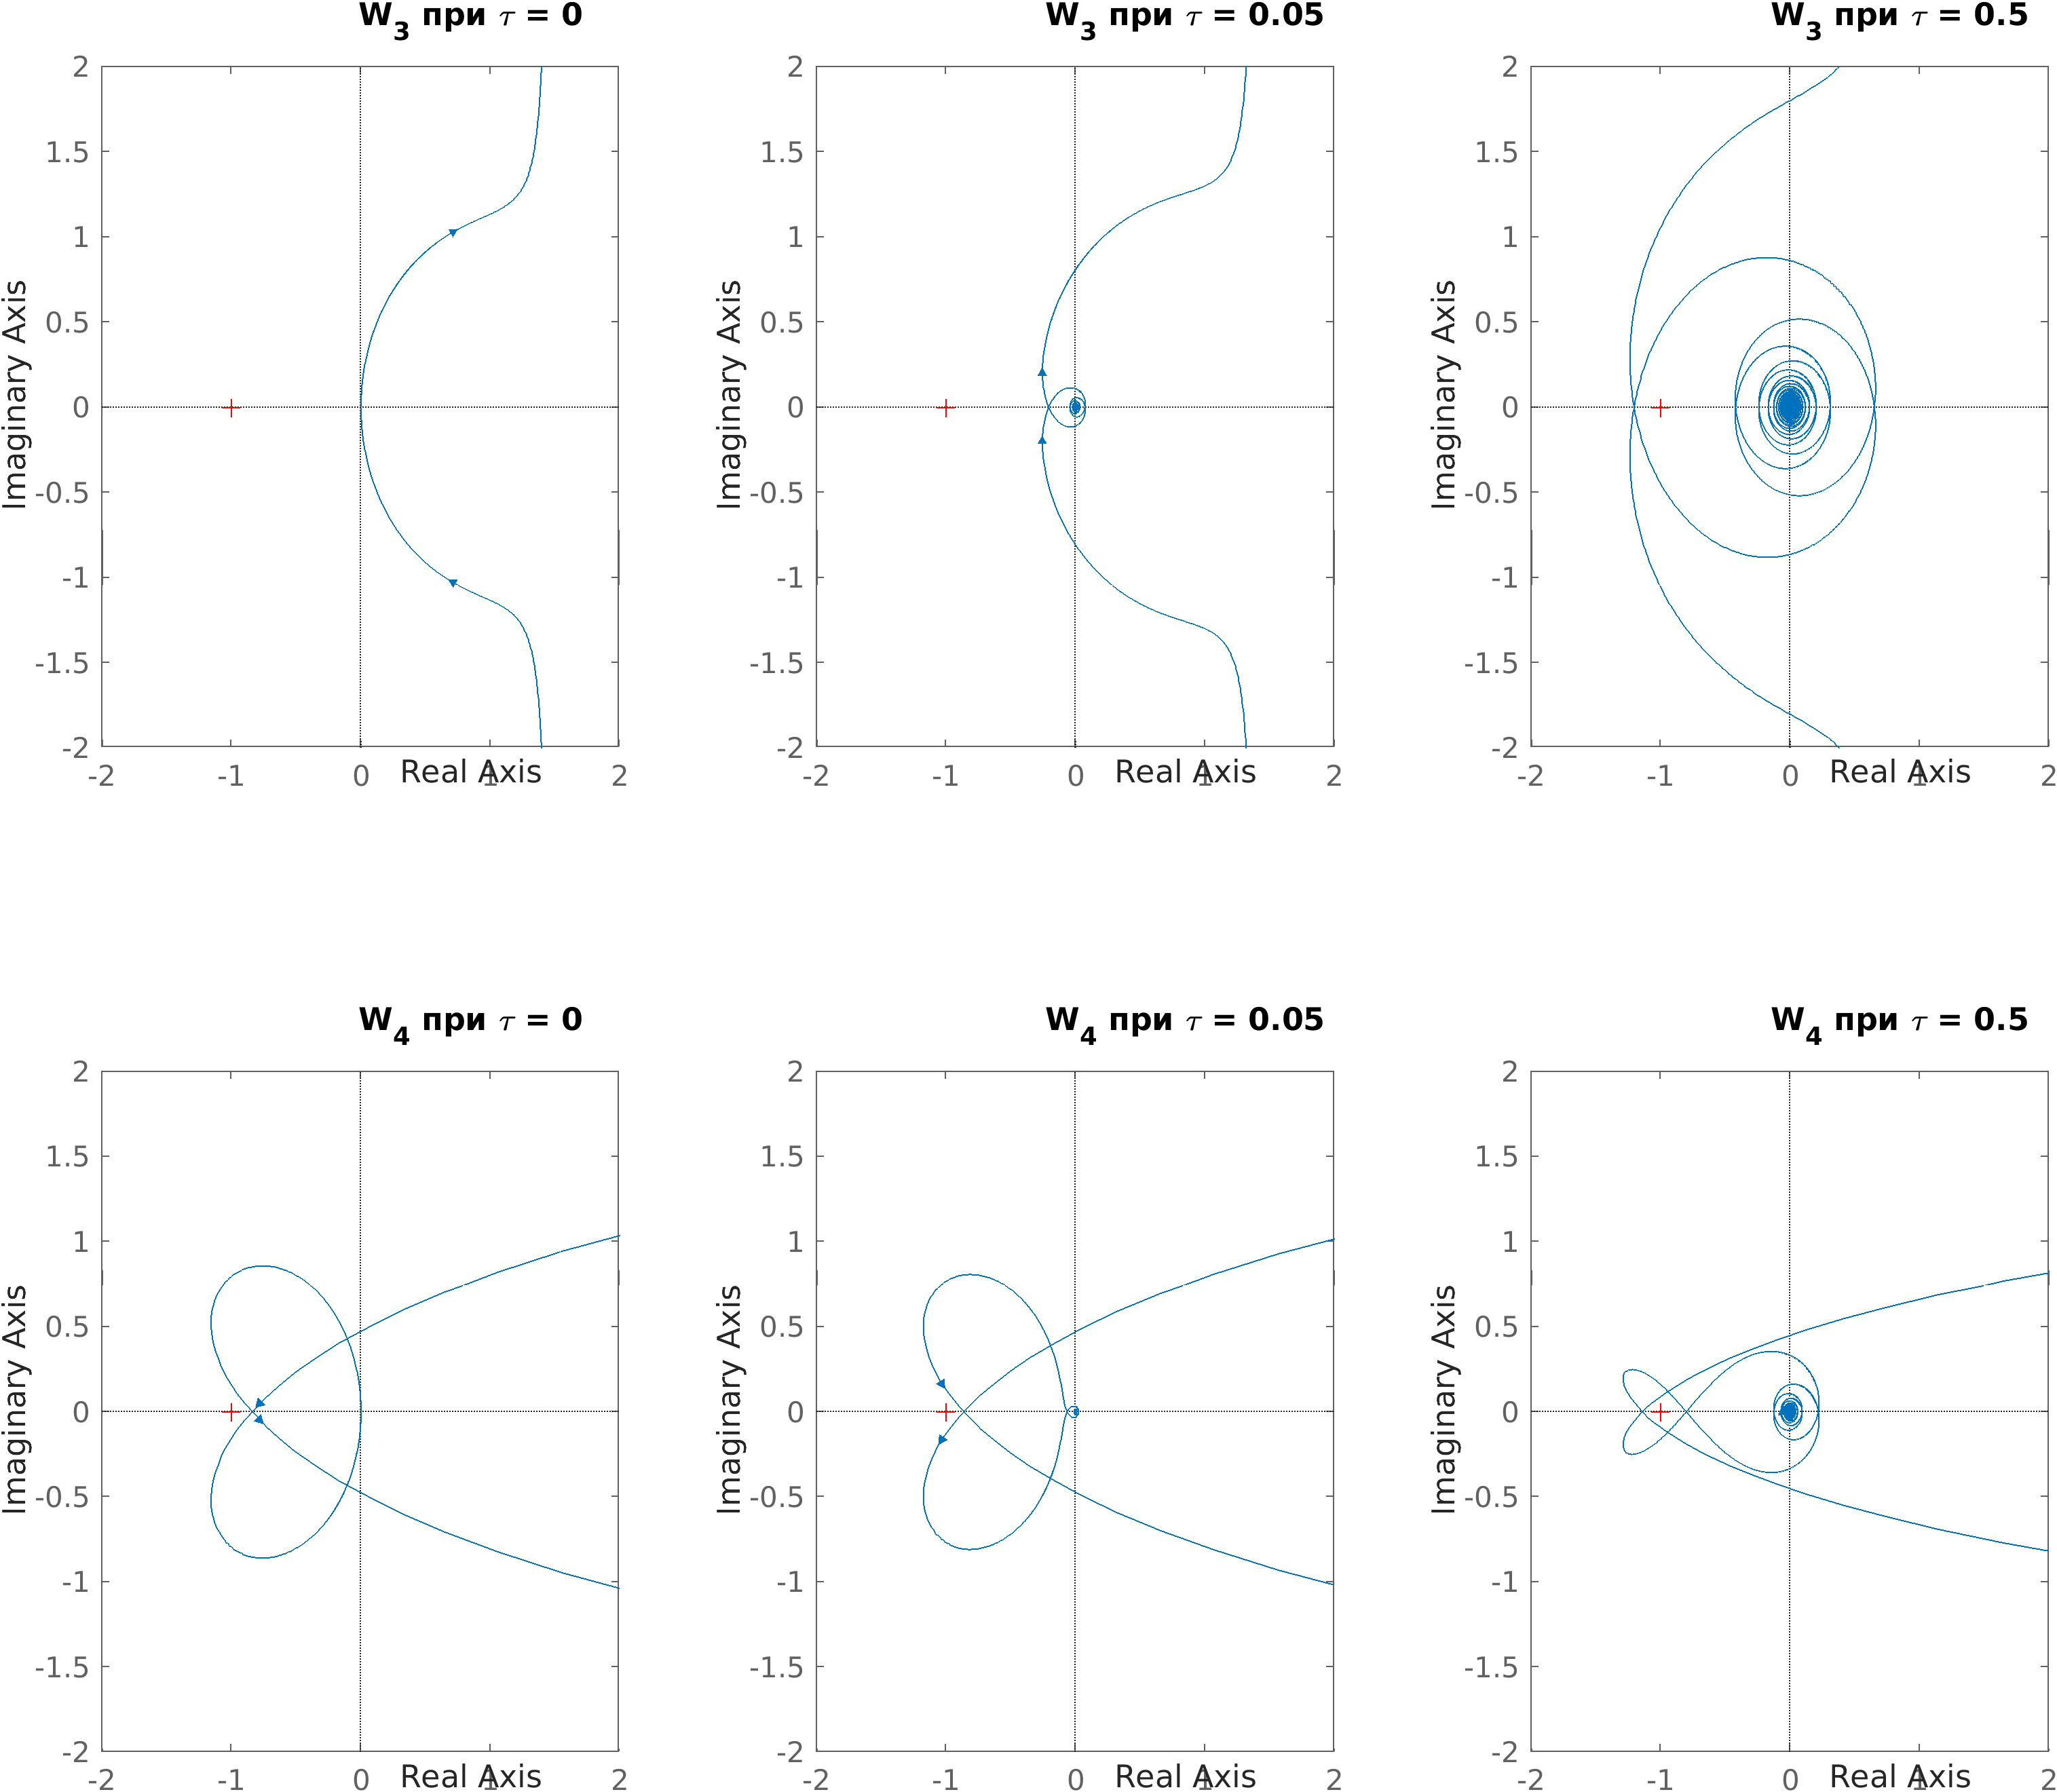
\includegraphics[width=\textwidth]{figs/task_3_taus_nyaquist.png}
    \caption{Годограф найквиста для $W_3$ и $W_4$ при разных запаздываниях}
    \label{fig:W34_nyquist}
\end{figure}
Найдем критическую частоту:
\begin{equation*}
    A(\omega_\text{кр})=1,
\end{equation*}
$$
25+49\omega_\text{кр}^2=\omega_\text{кр}^4+16\omega_\text{кр}^2,
$$
\begin{equation*}
    \omega_\text{кр}^4-33\omega_\text{кр}^2-25=0,
\end{equation*}
так как нас интересуют только вещественные и положительные частоты
\begin{equation*}
    \omega_\text{кр}^2=\frac{33+\sqrt{1189}}{2},
\end{equation*}
\begin{equation*}
    \omega_\text{кр}=\sqrt{16.5+\sqrt{297.26}}\approx 5.81.
\end{equation*}
Получили едсинственную частоту, что ожидаемо, так как если мысленно нарисовать
единичную окружность на годографе на рисунке \ref{fig:W34_nyquist} для $W_3$ и $\tau=0$,
то пересекать его будет только одна точна, если говорить только про положительные частоты.
Теперь можем найти максимальную задержку:
\begin{equation*}
    \varphi(\omega_\text{кр}) - \tau_{max}\omega_\text{кр}=-\pi,
\end{equation*}
\begin{equation*}
    -1.09-5.81\tau_{max}=-\pi,
\end{equation*}
\begin{equation*}
    \tau_{max} \approx 0.35,
\end{equation*}
и запас по фазе:
\begin{equation*}
    \varphi_\text{з}=\tau_{max}\omega_\text{кр}\approx 1.453\ \text{рад}\approx 83.2^{\circ} .
\end{equation*}
Получаем, что при $\tau<0.35$ система останется устойчивой, а при $\tau\geq 0.35$ 
станет неустойчивой. Проведем моделирование, которое можно посмотреть на рисунке \ref{fig:W3_steps}.
Выводи подтвердились, можно видеть как система становится все неустойчивее, и в конце концов
расходится.


\begin{figure}[H]
    \centering
    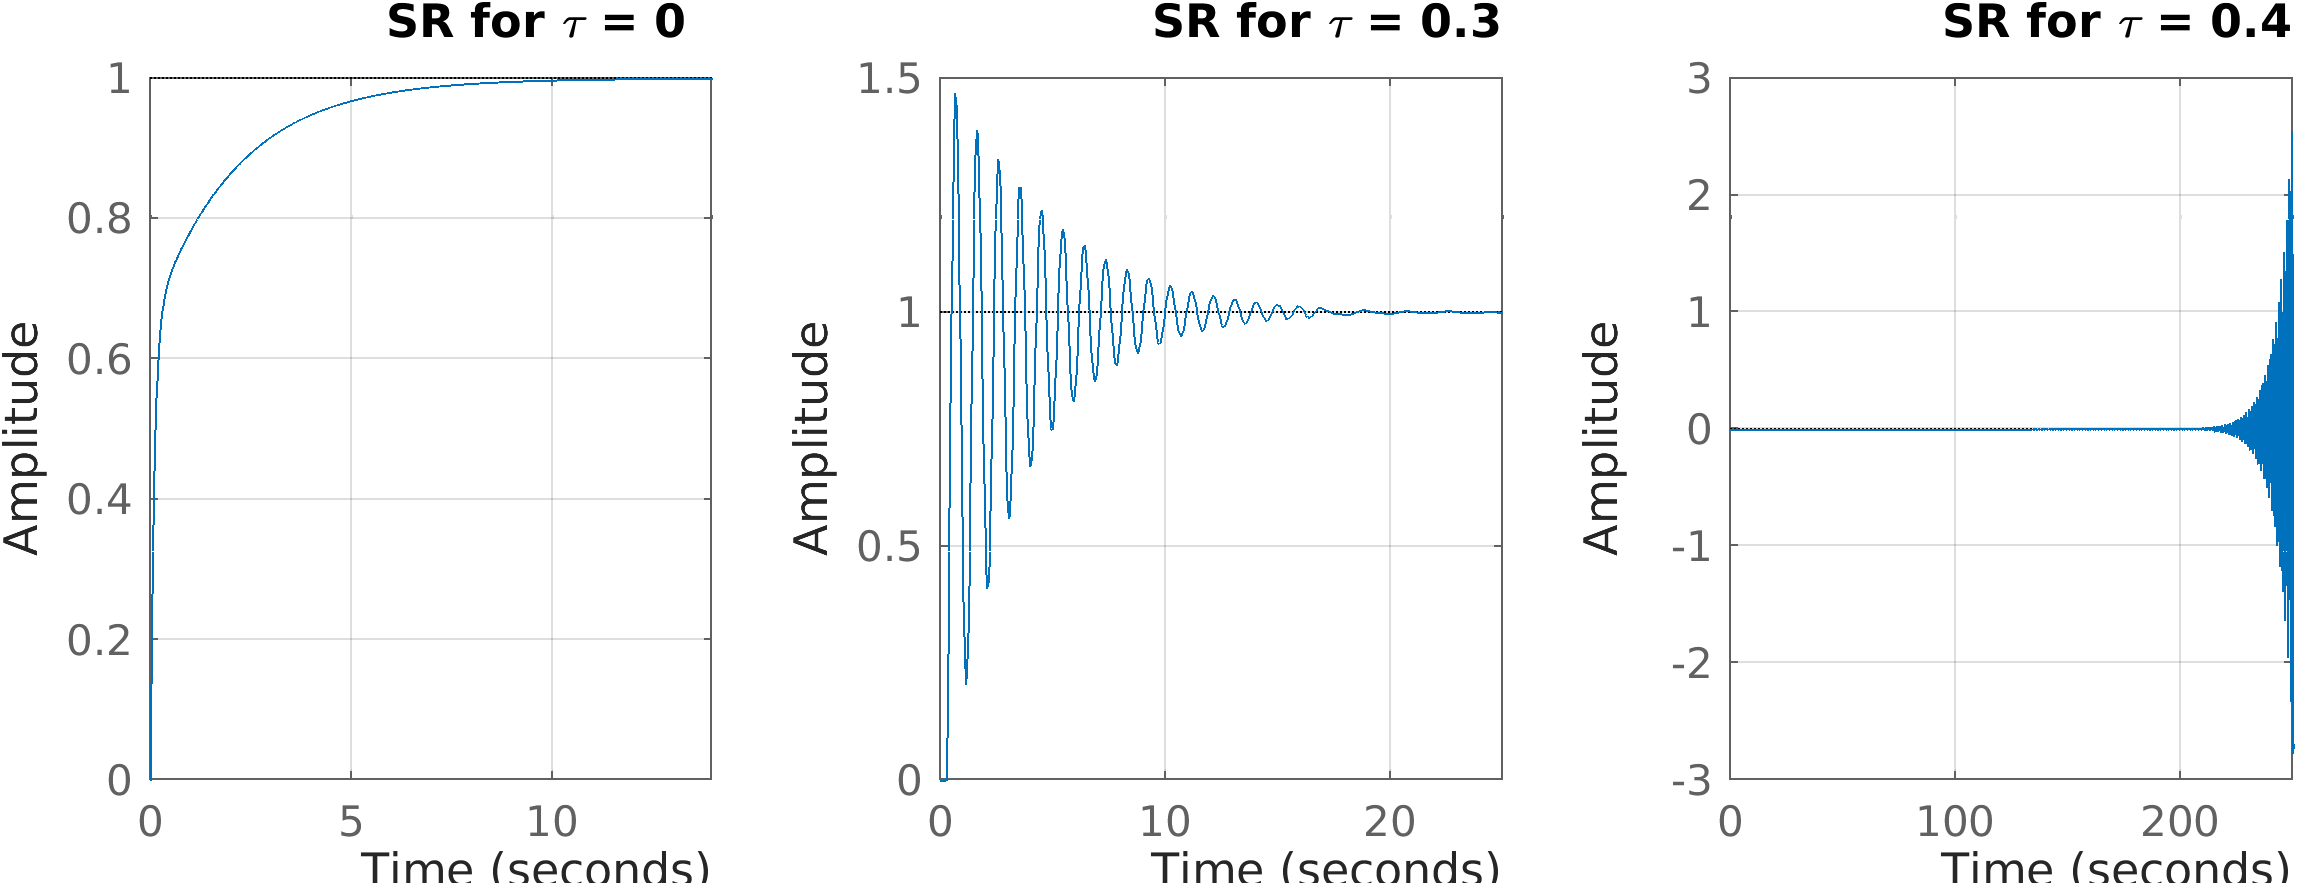
\includegraphics[width=\textwidth]{figs/task_3_W3_tausteps.png}
    \caption{Переходные харктеристики замкнутой $W_3$ при разных запаздываниях}
    \label{fig:W3_steps}
\end{figure}

\subsection{Четвертая ПФ}

Посмотрим на годограф четвертой ПФ, при закручивании точка (-1; 0) будет охвачиваться
против часовой стрелки, либо вообще не охвачиваться, это значит, что
замкнутая система имеет шанс стать устойчивой, так как неустойчивых корня два,
и по критерию Найквиста нужен один оборот против часовой для устойчивости. Рассмотрим ПФ:
\begin{equation*}
\begin{split}
    W_4(j\omega)&=\frac{-20\omega^2+1.6j\omega+2}{-10j\omega^3+10\omega-0.1j\omega+0.1}
    =\frac{\sqrt{(2-20\omega^2)^2+(1.6\omega)^2}}{\sqrt{(0.1+10\omega^2)^2}+(0.1\omega+10\omega^3)^2}\times\\
    &\times\exp \left( j \left[ \text{atan2}(1.6\omega,2-20\omega^2) - \text{atan2}(-0.1\omega-10\omega^3,0.1+10\omega^2) \right] \right).
\end{split}
\end{equation*}
Найдем критическую частоту:
\begin{equation*}
    \begin{split}
        A(\omega_\text{кр})&=1,\\
        (2-20\omega_\text{кр}^2)^2+(1.6\omega_\text{кр})^2&=(0.1+10\omega_\text{кр}^2)^2+(0.1\omega_\text{кр}+10\omega_\text{кр}^3)^2,\\
        4-80\omega_\text{кр}^2+400\omega_\text{кр}^4+2.56\omega_\text{кр}^2&=0.01+2\omega_\text{кр}^2+100\omega_\text{кр}^4+0.01\omega_\text{кр}^2+2\omega_\text{кр}^4+100\omega_\text{кр}^6,
    \end{split}
\end{equation*}
получаем
\begin{equation*}
    100\omega_\text{кр}^6-298\omega_\text{кр}^4+79.45\omega_\text{кр}^2-3.99=0,
\end{equation*}
положительные решения которого равны
\begin{equation*}
    \omega_{\text{кр}_0}\approx0.2576,\quad\omega_{\text{кр}_1}\approx0.4727,\quad\omega_{\text{кр}_2}\approx1.6402\ .
\end{equation*}
Фаза для них
\begin{equation*}
    \varphi(\omega_{\text{кр}_0})\approx0.8017,\quad\varphi(\omega_{\text{кр}_1})\approx3.2859,\quad\varphi(\omega_{\text{кр}_2})\approx4.1143\ .
\end{equation*}
Так как задержкой фазу мы можем только уменьшать, то первую можно "добить" до $-\pi$,
а оставшиеся до $\pi$. Найдем эти задержки:
\begin{equation*}
    \varphi(\omega_{\text{кр}_0})-\tau_0\omega_{\text{кр}_0}=-\pi,\quad
    \varphi(\omega_{\text{кр}_1})-\tau_1\omega_{\text{кр}_1}=\pi,\quad
    \varphi(\omega_{\text{кр}_2})-\tau_2\omega_{\text{кр}_2}=\pi\ ,
\end{equation*}
\begin{equation*}
    0.8017-0.2575\tau_0=-\pi,\quad
    3.2859-0.4727\tau_1=\pi,\quad
    4.1143-1.6402\tau_2=\pi\ ,
\end{equation*}
\begin{equation*}
    \tau_0=15.3138,\quad\tau_1=0.3053,\quad\tau_2=0.5930\ .
\end{equation*}
Исходя из критических частот и фаз предположу, что желанная задержка -- $\tau_1$,
тогда имеем такие интервалы для замкнутой системы: $\tau\in(0;0.3053)$ -- 
неусточива, $\tau\in(0.3053;0.5930)$ -- устойчива, $\tau\in(0.5930; +\infty)$ -- неусточива.
Чтобы удостовериться в выводах, построим переходную характеристику для
значений задержек до и после найденных. Результаты моделирования можно
увидеть на рисунках \ref{fig:W41_steps} и \ref{fig:W42_steps}. Выводы подтвердились.

\begin{figure}[H]
    \centering
    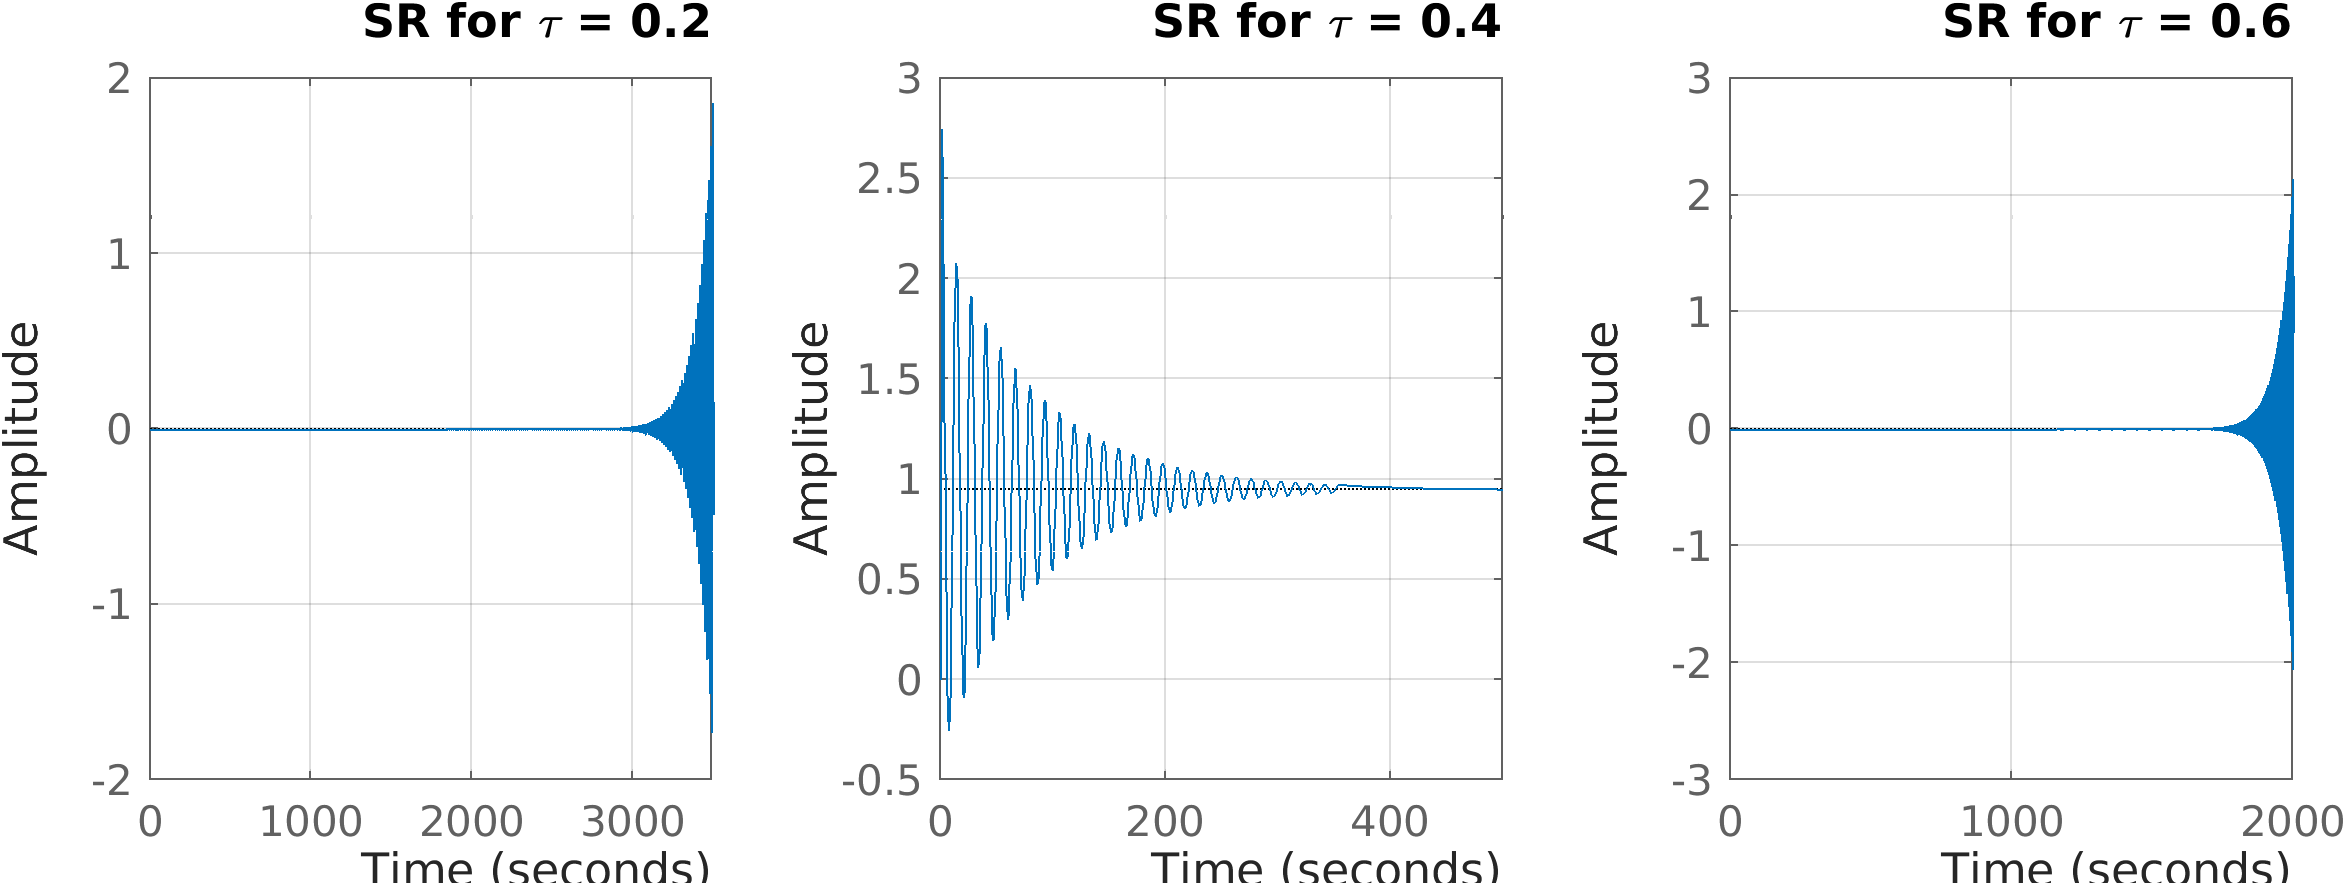
\includegraphics[width=\textwidth]{figs/task_3_W4_1_tausteps.png}
    \caption{Переходные характеристики замкнутой $W_4$ при $\tau\in\{0.2,0.4,0.6\}$}
    \label{fig:W41_steps}
\end{figure}

\begin{figure}[H]
    \centering
    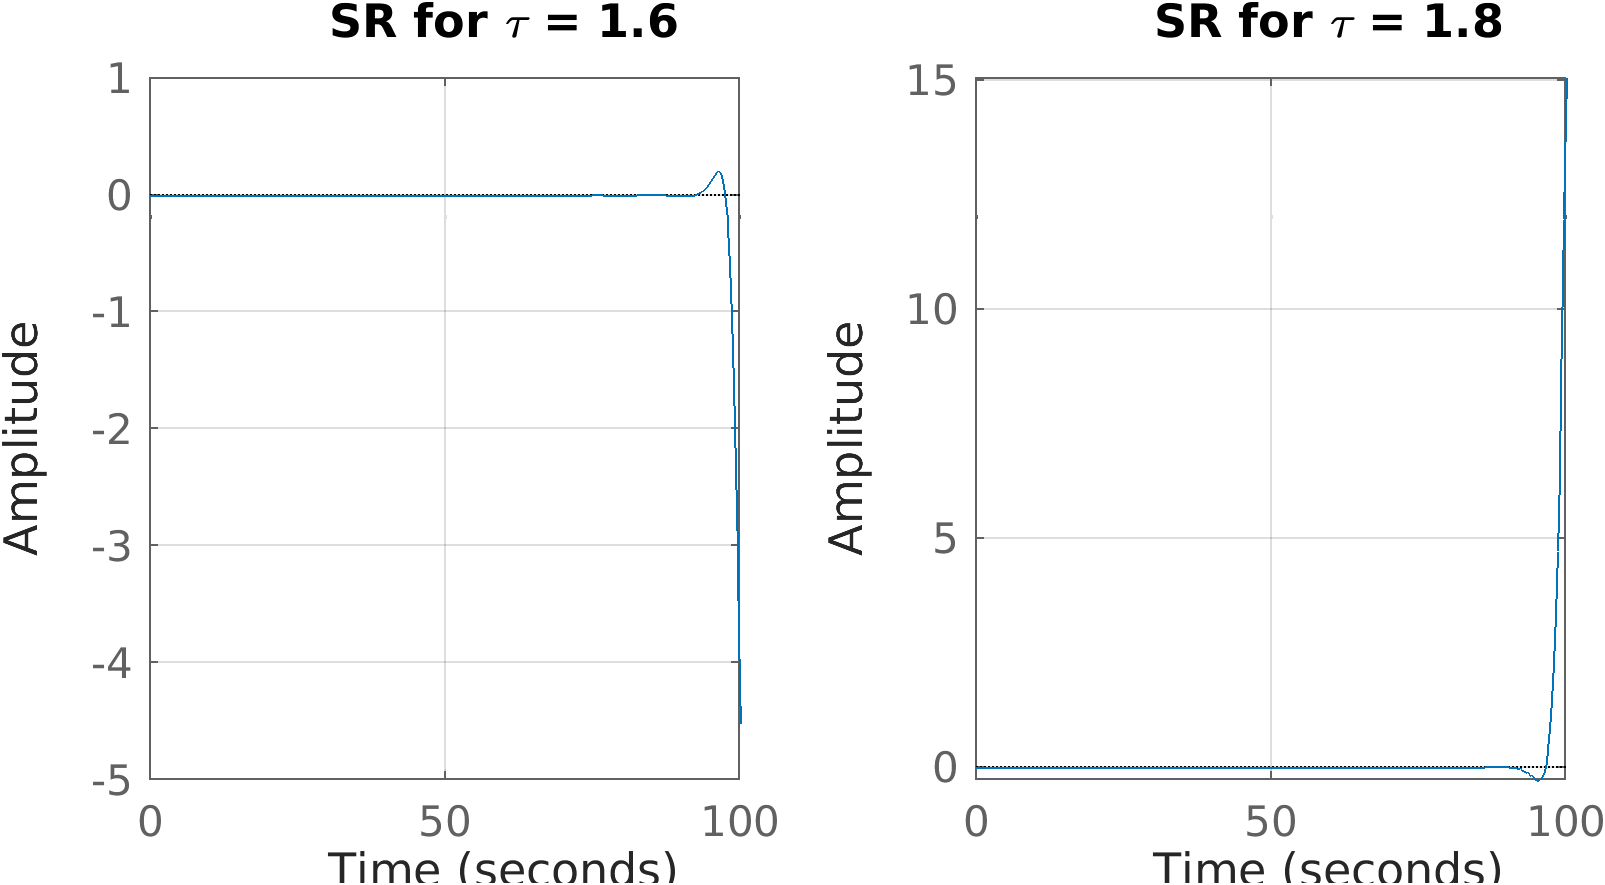
\includegraphics[width=0.8\textwidth]{figs/task_3_W4_2_tausteps.png}
    \caption{Переходные характеристики замкнутой $W_4$ при $\tau\in\{1.6,1.8\}$}
    \label{fig:W42_steps}
\end{figure}


\newpage
\section{Заключение}

В данной лабораторной работе были рассмотрены и исследованы 
различные передаточные функции с помощью годографа Найквиста.
Для некоторых функций были найдены интервалы для коэффициент 
усиления и запаздывания, при которых замкнутые системы или устойчивы, или
нейстойчивы.